\documentclass[a4paper,11pt,twoside]{style}

\usepackage{amsmath,amssymb}
\usepackage[latin1]{inputenc}
\usepackage[T1]{fontenc}
\usepackage[left=1.5in,right=1.3in,top=1.1in,bottom=1.1in,includefoot,includehead,headheight=13.6pt]{geometry}
\renewcommand{\baselinestretch}{1.04}
\usepackage{lipsum}
\usepackage[nottoc, notlof, notlot]{tocbibind}
\usepackage{minitoc}
\setcounter{minitocdepth}{2}
\usepackage{aecompl}
\usepackage{listings}
\usepackage{glossaries}

\lstdefinestyle{java}{
  language=Java,
  showspaces=false,
  showtabs=false,
  breaklines=true,
  showstringspaces=false,
  breakatwhitespace=true,
  commentstyle=\color{green},
  keywordstyle=\color{blue},
  stringstyle=\color{red},
  basicstyle=\scriptsize,
  moredelim=[il][\textcolor{grey}]{$$},
  moredelim=[is][\textcolor{grey}]{\%\%}{\%\%}
}

\usepackage{color}
\usepackage{verbatim}
\usepackage{xcolor}
\definecolor{GreyRowTable}{HTML}{EEEEEE}
\usepackage{mdframed} 
\usepackage[intoc]{nomencl}
\renewcommand{\nomname}{List of Abbreviations}
\makenomenclature
\usepackage{ifpdf}
\usepackage{url}
\ifpdf
  \usepackage[pdftex]{graphicx}
  \DeclareGraphicsExtensions{.jpg}
  \usepackage[a4paper,pagebackref,hyperindex=true]{hyperref}
\else
  \usepackage{graphicx}
  \DeclareGraphicsExtensions{.ps,.eps}
  \usepackage[a4paper,dvipdfm,pagebackref,hyperindex=true]{hyperref}
\fi
\usepackage[nolist,nohyperlinks]{acronym}
\renewcommand*{\backref}[1]{}
\renewcommand*{\backrefalt}[4]{%
\ifcase #1 %
(Not cited.)%
\or
(Cited on page~#2.)%
\else
(Cited on pages~#2.)%
\fi}
\renewcommand*{\backrefsep}{, }
\renewcommand*{\backreftwosep}{ and~}
\renewcommand*{\backreflastsep}{ and~}
\usepackage{color}
\definecolor{linkcol}{rgb}{0,0,0.4} 
\definecolor{citecol}{rgb}{0.5,0,0} 
\hypersetup
{
bookmarksopen=true,
pdftitle="thesis",
pdfauthor="Benjamin Danglot", 
pdfsubject="Behavioral Changes Detection", %subject of the document
%pdftoolbar=false, % toolbar hidden
pdfmenubar=true, %menubar shown
pdfhighlight=/O, %effect of clicking on a link
colorlinks=true, %couleurs sur les liens hypertextes
pdfpagemode=None, %aucun mode de page
pdfpagelayout=SinglePage, %ouverture en simple page
pdffitwindow=true, %pages ouvertes entierement dans toute la fenetre
linkcolor=linkcol, %couleur des liens hypertextes internes
citecolor=citecol, %couleur des liens pour les citations
urlcolor=linkcol %couleur des liens pour les url
}
\setcounter{secnumdepth}{3}
\setcounter{tocdepth}{2}
\newcommand{\pd}[2]{\frac{\partial #1}{\partial #2}}
\def\abs{\operatorname{abs}}
\def\argmax{\operatornamewithlimits{arg\,max}}
\def\argmin{\operatornamewithlimits{arg\,min}}
\def\diag{\operatorname{Diag}}
\newcommand{\eqRef}[1]{(\ref{#1})}

\usepackage{rotating}
\usepackage{fancyhdr}
\pagestyle{fancy}
\fancyfoot{}
\fancyhead[LE,RO]{\bfseries\thepage} 
\fancyhead[RE]{\bfseries\nouppercase{\leftmark}}  
\fancyhead[LO]{\bfseries\nouppercase{\rightmark}} 
\let\headruleORIG\headrule
\renewcommand{\headrule}{\color{black} \headruleORIG}
\renewcommand{\headrulewidth}{1.0pt}
\usepackage{colortbl}
\arrayrulecolor{black}
\fancypagestyle{plain}{
  \fancyhead{}
  \fancyfoot{}
  \renewcommand{\headrulewidth}{0pt}
}
\usepackage{algorithm}
\usepackage{algorithmicx}
\usepackage{algpseudocode}
\makeatletter
\def\cleardoublepage{\clearpage\if@twoside \ifodd\c@page\else%
  \hbox{}%
  \thispagestyle{empty}%              % Empty header styles
  \newpage%
  \if@twocolumn\hbox{}\newpage\fi\fi\fi}

\makeatother
\newcommand{\reviewtimetoday}[2]{\special{!userdict begin
    /bop-hook{gsave 20 710 translate 45 rotate 0.8 setgray
      /Times-Roman findfont 12 scalefont setfont 0 0   moveto (#1) show
      0 -12 moveto (#2) show grestore}def end}}
\newenvironment{maxime}[1]
{
\vspace*{0cm}
\hfill
\begin{minipage}{0.5\textwidth}%
%\rule[0.5ex]{\textwidth}{0.1mm}\\%
\hrulefill $\:$ {\bf #1}\\
%\vspace*{-0.25cm}
\it 
}%
{%

\hrulefill
\vspace*{0.5cm}%
\end{minipage}
}

\let\minitocORIG\minitoc
\renewcommand{\minitoc}{\minitocORIG \vspace{1.5em}}

\usepackage{multirow}

\newenvironment{bulletList}%
{ \begin{list}%
	{$\bullet$}%
	{\setlength{\labelwidth}{25pt}%
	 \setlength{\leftmargin}{30pt}%
	 \setlength{\itemsep}{\parsep}}}%
{ \end{list} }

\newtheorem{definition}{Definition}
\newtheorem{fact}{Fact}
\renewcommand{\epsilon}{\varepsilon}

% centered page environment

\newenvironment{vcenterpage}
{\newpage\vspace*{\fill}\thispagestyle{empty}\renewcommand{\headrulewidth}{0pt}}
{\vspace*{\fill}}

\usepackage{xspace}
\usepackage{lettrine}

% Landscape package
\usepackage{pdflscape}
% use \begin{landscape} and \end{landscape}

\newdimen\origiwspc%
\newdimen\origiwstr%
\origiwspc=\fontdimen2\font% original inter word space
\origiwstr=\fontdimen3\font% original inter word stretch

%
%   Can play with the following value to change words spacing
%
\fontdimen2\font=0.2ex% inter word space
\fontdimen3\font=0.1em% inter word stretch
\fontdimen2\font=\origiwspc% (original) inter word space
\fontdimen3\font=\origiwstr% (original) inter word stretch

% line spacing
\usepackage{setspace}
\renewcommand{\baselinestretch}{1.2}
%{\setstretch{1.0
%text
%}

\usepackage{afterpage}

\newcommand{\TODO}[1]{\textcolor{red}{#1}\GenericWarning{}{LaTeX Warning: TODO: #1}}\newcommand\todo\TODO

% ==========================================================
%		DSPOT 		COMMANDS
% ==========================================================

\newcommand{\algorithmautorefname}{Algorithm}
\newcommand{\Iampl}{\emph{I-Amplification}\xspace}
\newcommand{\Aampl}{\emph{A-Amplification}\xspace}
\newcommand{\dspot}{DSpot\xspace}
\newcommand{\DCI}{DCI\xspace}
\newcommand{\DCIA}{DCI-\Aampl\xspace}
\newcommand{\DCII}{DCI-\Iampl\xspace}
\newcommand{\etal}{\textit{et al.}\xspace}
\newcommand{\ie}{\textit{i.e.}\xspace}
\newcommand{\eg}{\textit{e.g.}\xspace}
\newcommand{\gh}{GitHub\xspace}
\newcommand{\pitest}{Pitest\xspace}
\newcommand{\xwiki}{XWiki\xspace}
\newcommand{\ms}{mutation score\xspace}
\newcommand{\ams}{number of killed mutants\xspace}
\newcommand{\junit}{JUnit\xspace}

\newcommand*\rotvertical{\rotatebox{-90}}
\newcommand*\rotverticalinv{\rotatebox{90}}
\newcommand*\rotlarge{\rotatebox{70}}
\newcommand*\rothalf{\rotatebox{45}}
\newcommand{\rot}[1]{\rotatebox{#1}}

\definecolor{ForestGreen}{RGB}{34,139,34}

\usepackage{etex}
\usepackage{graphicx}
\usepackage{xcolor}
\usepackage{listings}  
\usepackage{amsmath}
\usepackage{balance}
\usepackage{tabularx}
\usepackage{booktabs}% for \midrule
\usepackage{mdframed} 
\usepackage{verbatim} % adds environment for commenting out blocks of text & for better verbatim
%\usepackage{enumitem}
\usepackage{paralist}
\usepackage{listings}
\usepackage{courier}
\usepackage{xspace}
\usepackage{balance}
\usepackage{multirow}
\definecolor{ForestGreen}{RGB}{34,139,34}
\definecolor{lightgray}{RGB}{225,225,225}
\usepackage[]{pdfcomment}
\usepackage{float}
\usepackage{lscape}
\usepackage{rotating}
\usepackage{adjustbox}

% DCI PACKAGES

\usepackage{etex}
\usepackage{graphicx}
\usepackage{xcolor}
%[colorlinks,linkcolor=blue,citecolor=blue,urlcolor=blue]
\usepackage{listings}  
\usepackage{amsmath}
\usepackage{balance}
\usepackage{tabularx}
\usepackage{booktabs}% for \midrule
\usepackage{mdframed} 
\usepackage{verbatim} % adds environment for commenting out blocks of text & for better verbatim
\usepackage{paralist}
\usepackage{listings}
\usepackage{courier}
\usepackage{xspace}
\usepackage{balance}
\usepackage{multirow}
\definecolor{ForestGreen}{RGB}{34,139,34}
\usepackage[]{pdfcomment}
\usepackage{lscape}

%\usepackage{hyperref}
\usepackage[inline]{enumitem}
\usepackage{amsmath}

\usepackage{amssymb}% http://ctan.org/pkg/amssymb
\usepackage{pifont}% http://ctan.org/pkg/pifont
\newcommand{\cmark}{{\color{ForestGreen}\ding{51}}\xspace}%
\newcommand{\lcmark}{{\textbf{\color{green}\ding{72}}}\xspace}%
\newcommand{\xmark}{{\color{red}\ding{55}}\xspace}%

\newcommand{\java}{Java\xspace}
\newcommand{\ExAmplifier}{\textbf{Ex2Amplifier}\xspace}
\newcommand{\head}{\emph{Pull request}\xspace}
\newcommand{\base}{\emph{base}\xspace}
\newcommand{\aampl}{\textsc{AAMPL}\xspace}
%\newcommand{\seci}{\textbf{SECI}\xspace}
\newcommand{\catg}{\textbf{CATG}\xspace}
\newcommand{\sbampl}{\textsc{SBAMPL}\xspace}
\newcommand{\nbProjects}{4\xspace}
\newcommand{\nbPullRequests}{36\xspace}

\lstset{ %
	%  backgroundcolor=\color{white},   % choose the background color; you must add \usepackage{color} or \usepackage{xcolor}
	basicstyle=\small\ttfamily,        % the size of the fonts that are used for the code
	captionpos=b,                    % sets the caption-position to bottom
	commentstyle=\small\color{ForestGreen},    % comment style
	escapeinside={(*@}{@*)},          % if you want to add LaTeX within your code
	keywordstyle=\color{blue},       % keyword style
	stringstyle=\color{purple},       % keyword style
	numberstyle=\tiny\color{black}, % the style that is used for the line-numbers
	stepnumber=1,                    % the step between two line-numbers. If it's 1, each line will be numbered
	title=\lstname,                   % show the filename of files included with \lstinputlisting; also try caption instead of title
	language=Java,
	breakatwhitespace=false,         % sets if automatic breaks should only happen at whitespace
	breaklines=true,                 % sets automatic line breaking
	extendedchars=true,              % lets you use non-ASCII characters; for 8-bits encodings only, does not work with UTF-8
	%frame=single,                    % adds a frame around the code
	showspaces=false,                % show spaces everywhere adding particular underscores; it overrides 'showstringspaces'
	showstringspaces=false,          % underline spaces within strings only
	showtabs=false,                  % show tabs within strings adding particular underscores
	tabsize=1,                       % sets default tabsize to 2 spaces
	framexleftmargin=15pt,
	frame = single
}

\newcommand{\rev}[1]{\textcolor{orange}{#1}\GenericWarning{}{LaTeX Warning: Revision: #1}}

\newcommand{\RQ}[2]{\textbf{RQ{#1}}: #2}

%%% Hilighting commands
\definecolor{red}{rgb}{1,0,0}
\definecolor{green}{rgb}{0,1,0}
\definecolor{blue}{rgb}{0,0,1}
\definecolor{cyan}{rgb}{0.4,1,1}
\definecolor{orange}{rgb}{0.9,0.5,0}
\definecolor{dkgreen}{rgb}{0,0.6,0}
\definecolor{gray}{rgb}{0.5,0.5,0.5}
\definecolor{purple}{rgb}{0.58,0,0.82}
\usepackage{times}

%Hilighting commands:
\newcommand{\todox}[1]{{\color{red}\bf\em TODO: #1}}
\newcommand{\commentx}[1]{{\color{purple}\bf\em Comment: #1}}
\newcommand{\done}[1]{{\color{blue}\bf\em DONE: #1}}\newcommand\DONE\done
\newcommand{\hll}[1]{\textcolor{orange}{#1}}
\newcommand{\hlll}[1]{\textcolor{dkgreen}{#1}}

% enable line breaking in texttt 
\usepackage[htt]{hyphenat}

\newenvironment{chaptersummary}
{
	\begin{center}
		\begin{mdframed}
		\begin{large}
		}
		{ 
		\end{large}
		\end{mdframed}
	\end{center}
}
%--------------------------------------------------

    \newacronym{OCCI}{OCCI}{\textit{Open Cloud Computing Interface}}
	\newacronym{UML}{UML}{\textit{Unified Modeling Language}}
	\newacronym{MDD}{MDD}{\textit{Model Driven Development}}
	\newacronym{MDE}{MDE}{\textit{Model Driven Engineering}}
	\newacronym{OMG}{OMG}{\textit{Object Management Group}}
	\newacronym{MDA}{MDA}{\textit{Model Driven Architecture}}
	\newacronym{MoDMaCAO}{MoDMaCAO}{\textit{Model-Driven Configuration Management of Cloud Applications with OCCI}}
	\newacronym{DSL}{DSL}{\textit{Domain specific language}}
	\newacronym{IaaS}{IaaS}{\textit{Infrastructure-as-a-Service}}
	\newacronym{PaaS}{PaaS}{\textit{Platform-as-a-Service}}
	\newacronym{SaaS}{SaaS}{\textit{Software-as-a-Service}}
	\newacronym{CIM}{CIM}{\textit{Cloud-Enabled Computation Independent Model}}
	\newacronym{CPIM}{CPIM}{\textit{Cloud-Provider Independent Model}}
	\newacronym{CPSM}{CPSM}{\textit{Cloud-Provider Specific Model}}
	\newacronym{HPC}{HPC}{\textit{High Performance Computing}}
	\newacronym{VM}{VM}{\textit{Virtual Machine}}
	\newacronym{NIST}{NIST}{\textit{National Institute of Standards and Technology}}
	\newacronym{EMF}{EMF}{\textit{Eclipse Modeling Framework}}
	\newacronym{TOSCA}{TOSCA}{\textit{Topology and Orchestration Specification for Cloud Applications}}
	\newacronym{API}{API}{\textit{Application Programming Interface}}
	\newacronym{CRM}{CRM}{\textit{Cloud Resource Management}}
	\newacronym{LHC}{LHC}{\textit{Large Hadron Collider}}
	\newacronym{PDE}{PDE}{\textit{Partial Differential Equation}}
	\newacronym{SCF}{SCF}{\textit{Scientific Computation Framework}}
	\newacronym{CF}{CF}{\textit{Computation Framework}}
	\newacronym{HOT}{HOT}{\textit{Heat Orchestration Template}}
	\newacronym{ETL}{ETL}{\textit{Epsilon Transformation Language}}
	\newacronym{EGL}{EGL}{\textit{Epsilon Generation Language}}
	\newacronym{YAML}{YAML}{\textit{YAML Ain't Markup Language}}
	\newacronym{CAML}{CAML}{\textit{Cloud Application Modeling Language}}
	\newacronym{MPI}{MPI}{\textit{Message Passing Interface}}
	\newacronym{OpenFOAM}{OpenFOAM}{\textit{Open Field Operation and Manipulation}}
	\newacronym{CFD}{CFD}{\textit{Computational Fluid Dynamics}}
	\newacronym{OASIS}{OASIS}{\textit{Organization for the Advancement of Structured Information Standards}}
	\newacronym{CAMP}{CAMP}{\textit{Cloud Application Management for Platforms}}
	\newacronym{IOPS}{IOPS}{\textit{Input/Output Operations}}
	\newacronym{CIMI}{CIMI}{\textit{Cloud Infrastructure Management Interface}}
	\newacronym{XML}{XML}{\textit{Extensible Markup Language}}
	\newacronym{NFS}{NFS}{\textit{Network File System}}
	\newacronym{IDE}{IDE}{\textit{Integrated Development Environment}}
	\newacronym{CAMF}{CAMF}{\textit{Cloud Application Management Framework}}
	\newacronym{XSD}{XSD}{\textit{XML Schema Definition}}
	\newacronym{OGF}{OGF}{\textit{Open Grid Forum}}
	\newacronym{CML}{CML}{\textit{Cloud Modeling Language}}
	\newacronym{OOI}{OOI}{\textit{OpenStack OCCI Interface}}
	\newacronym{IoT}{IoT}{\textit{Internet of Things}}
	\newacronym{URI}{URI}{\textit{Uniform Resource Identifier}}
	\newacronym{FSM}{FSM}{\textit{Finite State Machine}}
	\newacronym{GAE}{GAE}{\textit{Google App Engine}}
	\newacronym{MDCE}{MDCE}{\textit{Model-driven Cloudware Engineering}}
	\newacronym{SPL}{SPL}{\textit{Software Product Line}}
	\newacronym{REST}{REST}{\textit{REpresentational State Transfer}}
	\newacronym{CDMI}{CDMI}{\textit{Cloud Data Management Interface}}
	\newacronym{DSML}{DSML}{\textit{Domain-Specific Modeling Language}}
	\newacronym{GPL}{GPL}{\textit{General-Purpose Language}}
	\newacronym{OCL}{OCL}{\textit{Object Constraint Language}}
	\newacronym{BNF}{BNF}{\textit{Backus-Naur Form}}
	\newacronym{MOF}{MOF}{\textit{Meta-Object Facility}}
	\newacronym{GMF}{GMF}{\textit{Graphical Modeling Framework}}
	\newacronym{SOAP}{SOAP}{\textit{Simple Object Access Protocol}}
	\newacronym{WSDL}{WSDL}{\textit{Web Services Description Language}}
	\newacronym{UDDI}{UDDI}{\textit{Universal Description, Discovery and Integration}}
	\newacronym{CRUD}{CRUD}{\textit{Create, Retrieve, Update and Delete}}
	\newacronym{AWS}{AWS}{\textit{Amazon Web Services}}
	\newacronym{GCP}{GCP}{\textit{Google Cloud Platform}}
	\newacronym{SDK}{SDK}{\textit{Software Development Kit}}
	\newacronym{OVF}{OVF}{\textit{Open Virtualization Format}}
	\newacronym{DMTF}{DMTF}{\textit{Distributed Management Task Force}}
	\newacronym{MIT}{MIT}{\textit{Massachusetts Institute of Technology}}
	\newacronym{MOCCA}{MOCCA}{\textit{MOve to Clouds for Composite Applications}}
	\newacronym{CAMEL}{CAMEL}{\textit{Cloud Application Modeling and Execution Language}}
	\newacronym{EGI FC}{EGI FC}{\textit{European Grid Infrastructure Federated Clouds}}
	\newacronym{EGI}{EGI}{\textit{European Grid Infrastructure}}
	\newacronym{SLA}{SLA}{\textit{Service Level Agreement}}
	\newacronym{FM}{FM}{\textit{Feature Model}}
	\newacronym{VAT}{VAT}{\textit{Virtual Architecture Topology}}
	\newacronym{XaaS}{XaaS}{\textit{Everything as a Service}}
	\newacronym{FODA}{FODA}{\textit{Feature Oriented Domain Analysis}}
	\newacronym{ADM}{ADM}{\textit{Architecture-Driven Modernization}}
	\newacronym{CloudMF}{CloudMF}{\textit{Cloud Modeling Framework}}
	\newacronym{CSP}{CSP}{\textit{Constraint Satisfaction Problem}}
	\newacronym{CRTP}{CRTP}{\textit{Compute Resource Templates Profile}}
	\newacronym{URN}{URN}{\textit{Uniform Resource Name}}
	\newacronym{CLI}{CLI}{\textit{Command-Line Interface}}
	\newacronym{OMCRI}{OMCRI}{\textit{Open Mobile Cloud Robotics Interface}}
	\newacronym{IoE}{IoE}{\textit{Internet of Everything}}
	\newacronym{BRS}{BRS}{\textit{Bigraphical Reactive Systems}}
	\newacronym{PSIF}{PSIF}{\textit{PaaS Semantic Interoperability Framework}}
	\newacronym{CTS}{CTS}{\textit{Cloud target Selection}}
	\newacronym{SRL}{SRL}{\textit{Scalability Rules Languages}}
	\newacronym{CEM}{CEM}{\textit{Cloud Environment Model}}
	\newacronym{CDO}{CDO}{\textit{Cloud Deployment Option}}
	\newacronym{AMQP}{AMQP}{\textit{Advanced Message Queuing Protocol}}
	\newacronym{FCA}{FCA}{\textit{Formal Concept Analysis}}
	\newacronym{NLP}{NLP}{\textit{Natural Language Processing}}
	\newacronym{PoS}{PoS}{\textit{Word Tagging/Part-of-Speech}}
	\newacronym{RFC}{RFC}{\textit{Request For Comments}}
	\newacronym{CDSMS}{CDSMS}{\textit{Cloud Domain-Specific Modeling Studio}}
	\newacronym{PIA}{PIA}{\textit{Programme d'Investissements d'Avenir}} 
	\newacronym{RaaS}{RaaS}{\textit{Robot as a Service}} 
	\newacronym{CaaS}{CaaS}{\textit{Container as a Service}} \newacronym{CSAR}{CSAR}{\textit{Cloud Service ARchive}}
    \newacronym{PDP}{PDP}{\textit{Platform Deployment Package}} 
    \newacronym{MAPO}{MAPO}{\textit{Mining API usage Pattern from Open source repositories}}
    \newacronym{MDAC}{MDAC}{\textit{Model-Driven Approaches for the Cloud}}
    \newacronym{LTL}{LTL}{\textit{Linear Temporal Logic}}
    




\begin{document}

\begin{titlepage}
\begin{center}
\vspace*{-2cm}
\begin{figure}[!htbp]
  \begin{center}
  	\TODO{PUT SOME LOGOS}
  \end{center}
\end{figure}
\hrule


%\noindent {\large \textbf{UNIVERSITY OF Lille}} \\
\vspace*{0.9cm}
\noindent {\Huge \textbf{Behavioural Change Detection}} \\
\vspace*{0.9cm}
\vspace*{0.5cm}
\noindent \Huge \textbf{P H D\ \ T H E S I S} \\
\vspace*{0.3cm}
\noindent \large {to obtain the title of} \\
\vspace*{0.3cm}
\noindent \LARGE \textbf{PhD of Science} \\
\vspace*{0.3cm}
%\noindent \Large of the University of Lille \\
\noindent \Large \textbf{Specialty : \textsc{Computer Science}}\\
\vspace*{0.4cm}
\noindent \large {Defended on \todo{xx}\\}
\noindent \LARGE \textbf{Benjamin \textsc{Danglot}} \\
\vspace*{0.9cm}
\noindent \Large prepared at Inria Lille-Nord Europe, \textsc{Spirals} Team\\
\vspace*{0.5cm}
\end{center}
\noindent \large \textbf{Thesis committee:} \\
\begin{center}
\noindent \large 
\begin{tabular}{llcl}
      \textit{Supervisors:}	& Martin \textsc{Monperrus}	& - & KTH Royal Institute of Technology \\
      & Lionel \textsc{Seinturier}	& - & Univeristy of Lille \\
      \textit{Reviewers:} &  & - & \\
      \textit{Examiner:} &  & - & \\
      \textit{Chair:} &  & - & \\
      \textit{Invited:}	& Benoit \textsc{Baudry} & - &  KTH Royal Institute of Technology\\
      & Vincent \textsc{Massol} & - &  XWiki
\end{tabular}
\end{center}
\end{titlepage}
\sloppy

\titlepage


\dominitoc

\pagenumbering{roman}

\cleardoublepage

 \begin{flushright}
\textit{``O sed fugit interea fugit irreparabile tempus audeamus nunc.''}\\
-- Ril\'es
\end{flushright}
\cleardoublepage

\dedicatory{TODO}
\cleardoublepage

\section*{Acknowledgements}

\begin{vcenterpage}
	\todo{write it}
\end{vcenterpage}%\printnomenclature

\cleardoublepage

\section*{Abstract}

\begin{vcenterpage}
	\todo{write it}
\end{vcenterpage}
-Ah non il ne faut pas confondre identité de couleur et expression de couleur...
Show less


\cleardoublepage

\section*{Publications}

	\todo{write it}
	
\cleardoublepage

\section*{R\'esum\'e}

	\todo{write it}

\cleardoublepage

\tableofcontents
\addcontentsline{toc}{chapter}{\listfigurename}
\mtcaddchapter
\listoffigures
\addcontentsline{toc}{chapter}{\listtablename}
\mtcaddchapter
\listoftables

\mainmatter

\chapter{Introduction}

\section{Background and Motivations}

\section{STAMP-project}
\chapter{State of the Art}
\label{chap:sota}

\cite{survey:amplification}
\chapter{\dspot: A Test Amplification Tool}
\label{chapter:dspot}

\begin{chaptersummary}
		In this chapter, I expose the major output of this thesis: \dspot.
		\dspot is a test amplification tool that have the ambition to improve the test suite of real projects, and the global quality of continuous integration process.
		\dspot achieves this by providing a set of automated procedures done in three majors step:\\
		1) it modifies the test inputs in order to trigger new behavior.\\
		2) it generates assertions to verify the new behavior of the program.\\
		3) it selects amplified test methods according to a specific test-criterion such as branch coverage.\\
		\dspot's output is a set of amplified test methods that improve the original test suite according to the specified test-criterion.\\
		In this chapter, I first define key concepts in \autoref{sec:dspot:definitions};
		Then, I expose an overview of \dspot with its principle, input, output, and its workflow in \autoref{sec:dspot:overview};
		Followed by explanation of \dspot's algorithm in \autoref{sec:dspot:algorithm};
		Eventually, I detail the implementation and the ecosystem of \dspot in \autoref{sec:dspot:implemention}.
\end{chaptersummary}

\minitoc

\graphicspath{{.}{chapitres/dspot/}}

% ---------------------------------------------------------------------------------------
% definitions
% ---------------------------------------------------------------------------------------
\section{Definitions}
\label{sec:dspot:definitions}

We first define the core terminology of \dspot in the context of object-oriented Java programs.

\textbf{Test suite} is a set of test classes.

\textbf{Test class} is a class that contains test methods. A test class is neither deployed nor executed in production.

\textbf{Test method} or \textbf{test case} is a method that sets up the system under test into a specific state and checks that the actual state at the end of the method execution is the expected state.

\textbf{Unit test} is a test method that specifies a targeted behavior of a program. 
Unit tests are usually independent from each other and execute a small portion of the code, \ie a single unit or a single component of the whole system.

\textbf{System test} or \textbf{Integration test} is a test method that specifies a large and complex behavior of a program.
System tests are usually large, long to be executed and use a lot of different component of the program.

\textbf{Test-criterion} is a measure of the quality of the test suite according to an engineering goal.
For instance, one can measure the execution speed of its test suite, and consider that the faster it is executed the better it is.
The most popular would be probably the execution coverage, which can be measured a different level: branches, statements, instructions.
It measures the proportion of the program that the test suite executes.
The more it executes, the better is considered the test suite since it is likely to verify more behavior.

\textbf{Amplified test suite} is an existing test suite to which we add amplified test methods.

\textbf{Amplified test method} is a test method that has been amplified, \ie it has been obtained using an test amplification process and an existing test method.

\textbf{Test input} is the first key component of test methods. 
It is responsible to set the program into a specific state using objects, method calls and literals.

\textbf{Assertion} or \textbf{oracle} is the second key component of test methods. 
It is responsible to verify that the state of the program, when the test input (the first component) is executed, is the expected one. 
It takes the form of comparison between hard-coded values and program's values, or the presence / absence of errors.

\section{Overview}
\label{sec:dspot:overview}

\subsection{Principle}
\label{subsec:dspot:overview:principle}

\begin{figure}[h]
	\centering
	\fbox{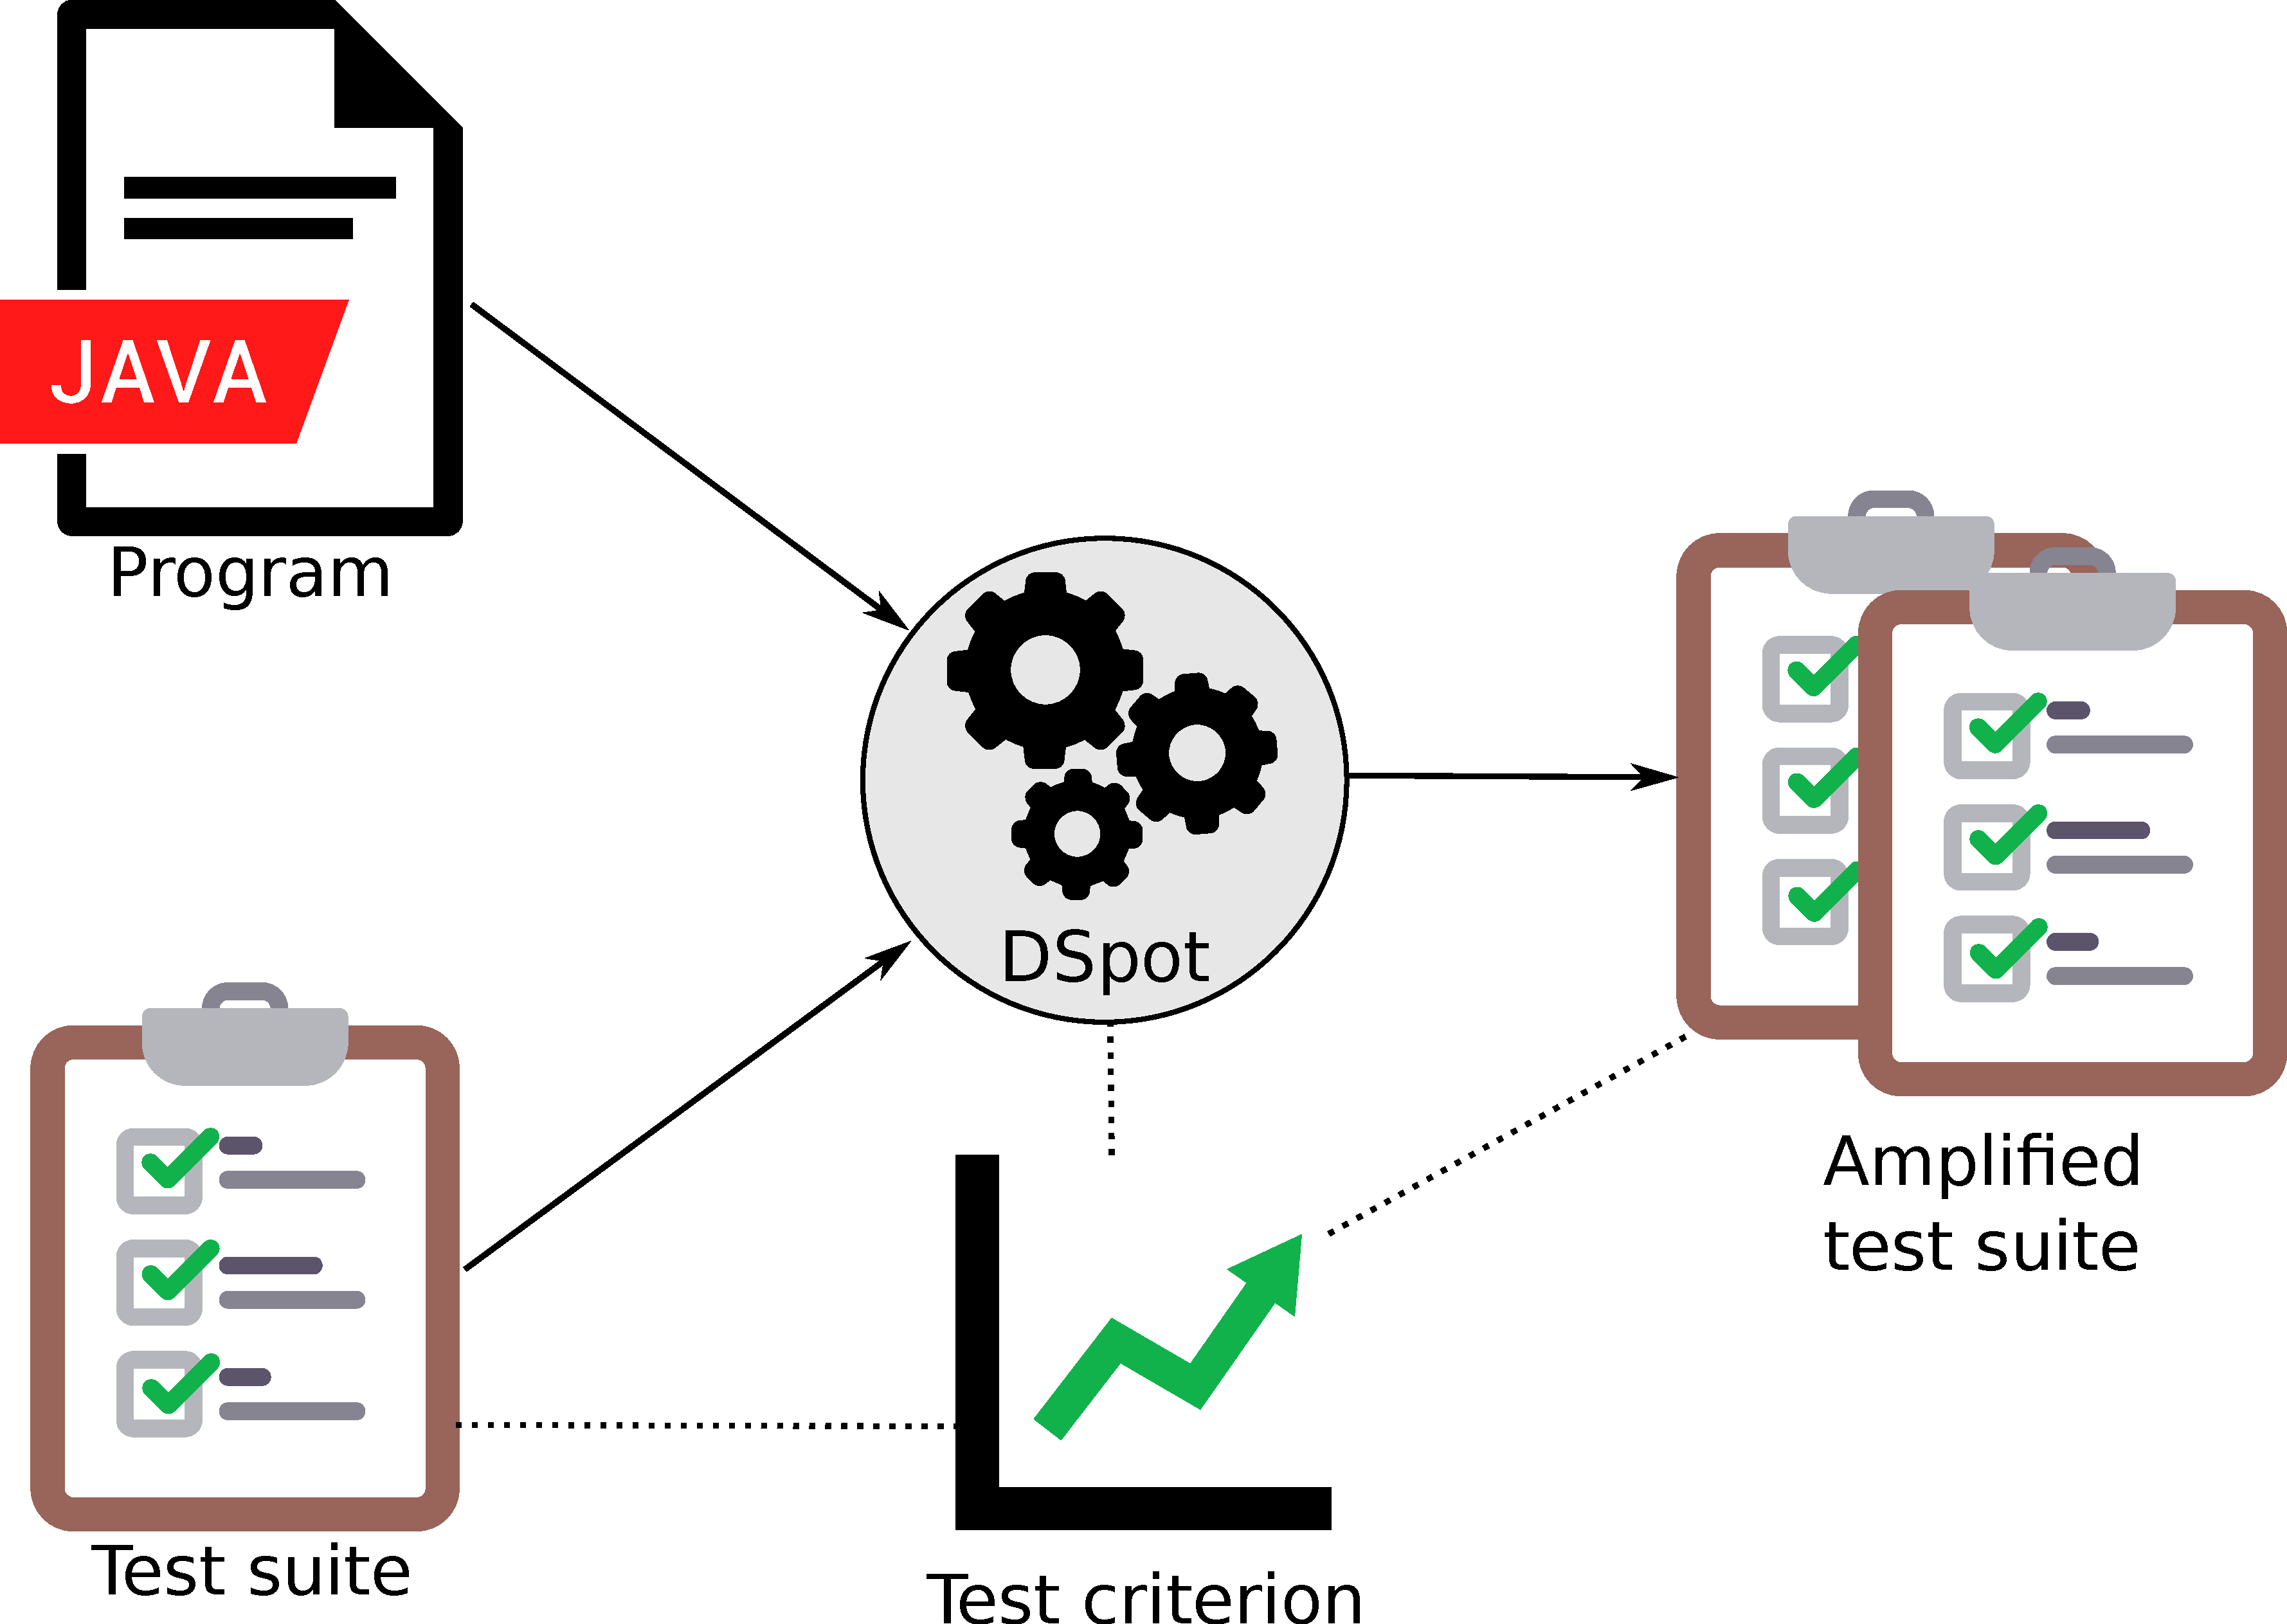
\includegraphics[width=.6\linewidth]{dspot_principle.pdf}}
	\caption{
		\dspot's principle: \dspot takes as input a program, an existing test suite, and a test-criterion. 
		\dspot outputs a set of amplified test methods.
		When added to the existing test suite, these amplified test methods increase the test-criterion, \ie the amplified test suite is better than the original one.
	}
	\label{fig:dspot:principle}
\end{figure}

DSpot is a test amplification tool.
Its goal is to improve an existing test suite according to a specific test-criterion.
DSpot takes as input the program, an existing test suite, and a test-criterion. 
The output of DSpot is a set of amplified test methods that are variants of existing test methods.
When added to the existing test suite, it create an \emph{amplified test suite}.
This amplified test suite is better than the original test suite according to the test-criterion used during the amplification.
For instance, one amplifies its test suite using branch coverage as test-criterion.
This amplified test suite will execute more branches than the exiting test suite, \ie the one without amplified test methods.

\dspot's principle is summarize in \autoref{fig:dspot:principle}.

\subsection{Input}
\label{subsec:dspot:overview:input}

\dspot's inputs are a program, a set of existing test methods and a test-criterion.
The program is used as ground truth: in \dspot we consider the program used during the amplification correct.
The existing test methods are used as a seed for the amplification.
\dspot applies transformation individually to these test methods in order to improve the overall quality of the test suite with respect to the specified test-criterion.

\subsection{Output}
\label{subsec:dspot:overview:output}

\dspot produces variants of the test methods provided as input.
We call these variants \emph{amplified test methods}, since there are test methods that has been obtained using an amplification process.
These amplified test methods are meant to be added to the test suite.
By adding amplified test methods to the existing test suite, it creates an amplified test methods that improve the overall test suite quality.
By construction, the amplified test suite is at least as good, or better than the original one with respect to the specified criterion.

An amplified test method's integration can be done in two way:
1) the developer integrates as it is the amplified test method into the test suite;
2) the developer integrate only the changes between the original test method and the amplified test method.
This enrich directly an existing test method.

\begin{figure}[h]
	\centering\fbox{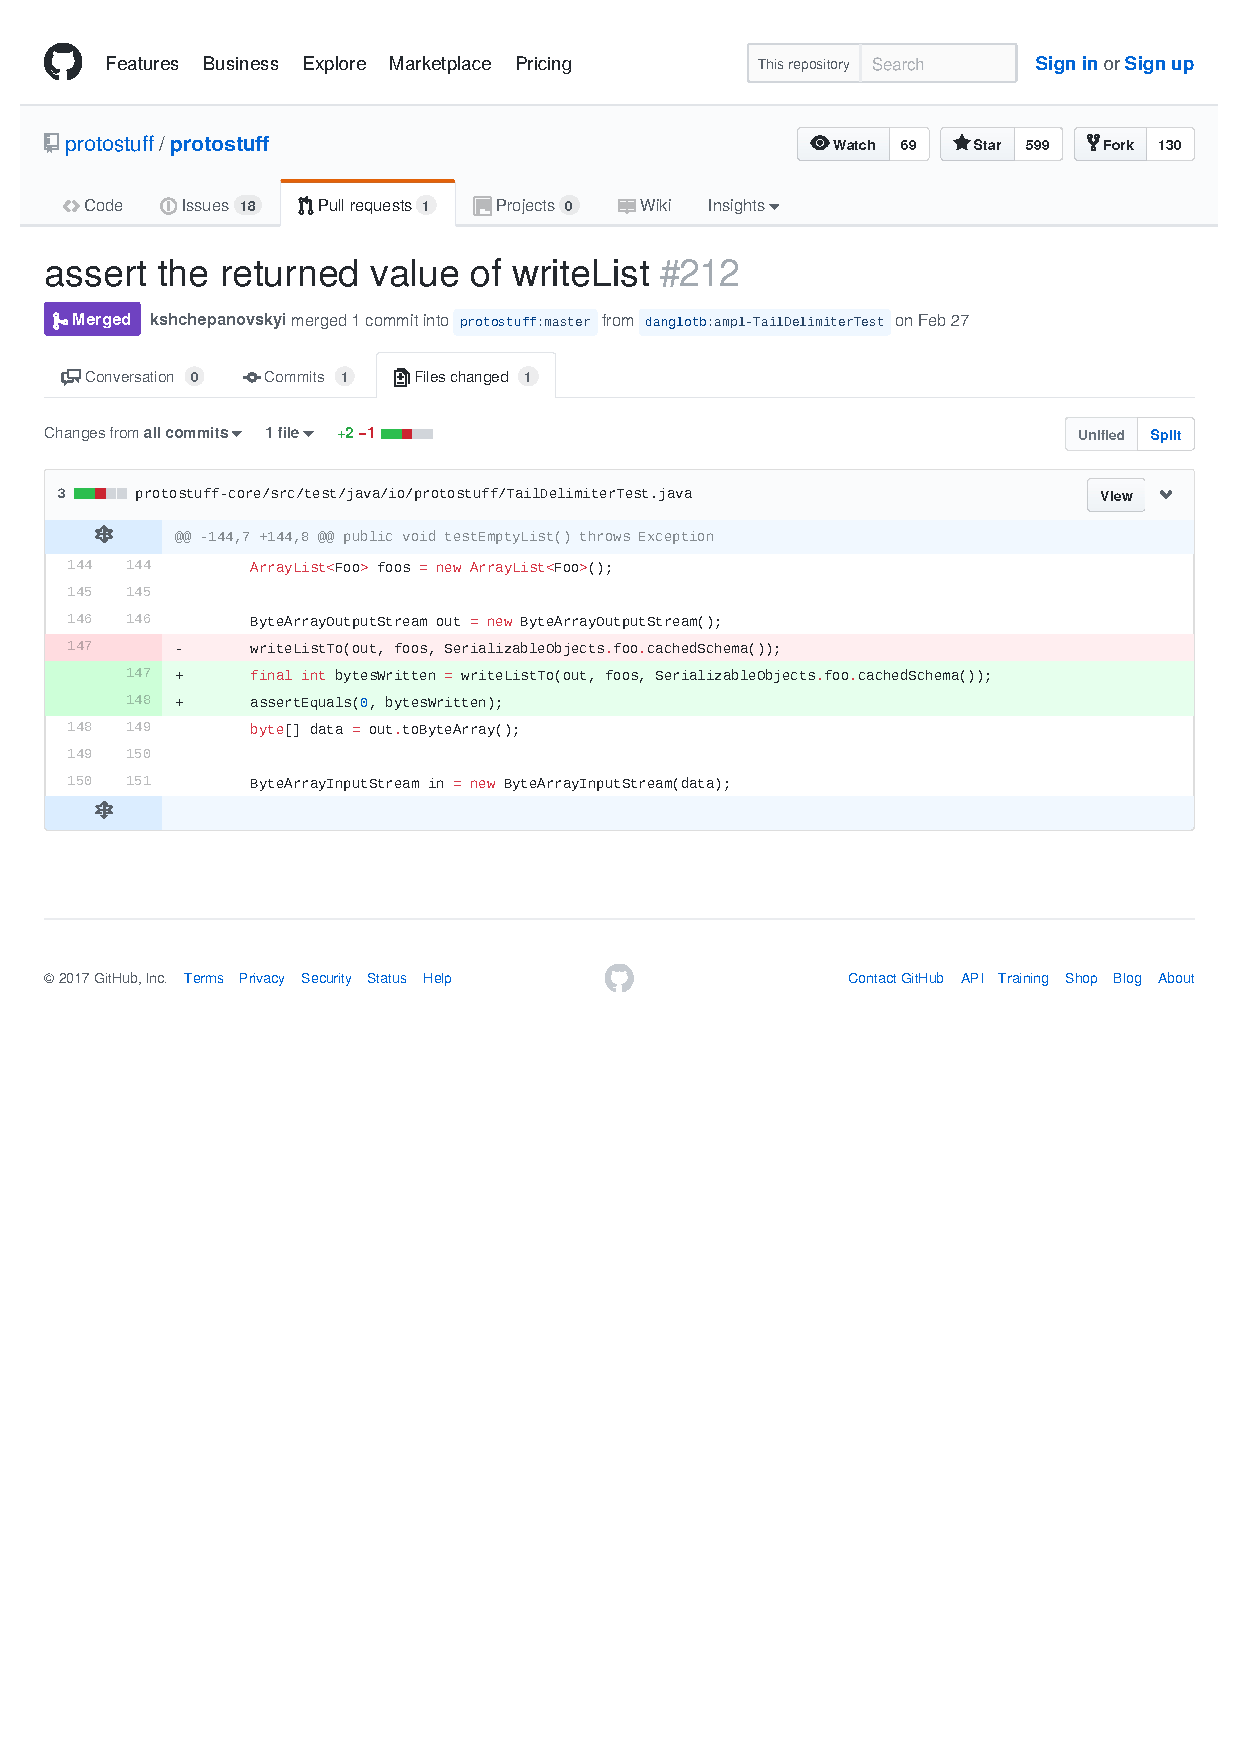
\includegraphics[width=0.98\textwidth, trim=4.15cm 17.52cm 4.05cm 10.76cm, clip]{protostuff.pdf}}
	\caption{Example of what \dspot produces: a diff to improve an existing test case.}
	\label{fig:diff-protostuff}
\end{figure}

\autoref{fig:diff-protostuff} shows an example of changes' set obtained using DSpot.

By construction, all \dspot's amplification can be represented as a diff on an existing test method since amplified test methods are variants of existing ones.

\subsection{Workflow}
\label{subsec:dspot:overview:workflow}

\begin{figure}[h]
	\centering\fbox{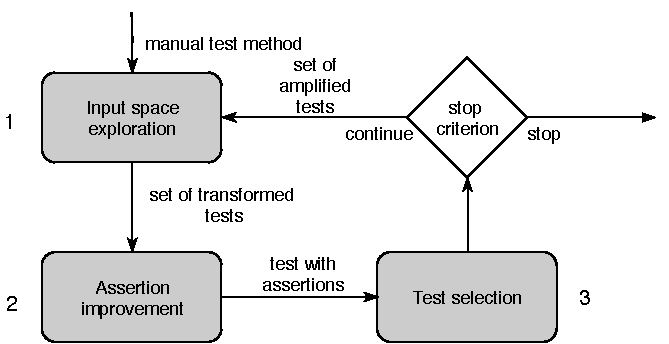
\includegraphics{dspot-workflow.pdf}}
	\caption{DSpot's workflow in three main steps: 1) the modification of test code's inputs, called ``input space exploration''; 2) the addition of new assertions called ``assertion improvement''; 3) the amplified test methods selection}
	\label{fig:dspot-workflow}
\end{figure}

The main workflow of \dspot is composed of 3 main phases:
1) the modification of test code's inputs inspired by Tonella's technique~\cite{tonella}, called ``input space exploration''; 
this phase consists in modifying test values (\eg literals), objects and methods calls, the underlying details will be explained in details in \autoref{subsec:dspot:algorithm:input-space-exploration}.
2) the addition of new assertions per Xie's technique~\cite{TaoXie2006}, this phase is called ``assertion improvement''.
The behavior of the system under test is considered as the oracle of the assertion, see \autoref{subsec:dspot:algorithm:new-assertions}.
In \dspot, the combination of both techniques, \ie the combination of input space exploration and assertion improvement is called ``test amplification''.
3) the amplified test methods selection according to a given test-criterion, \eg branch coverage.

\subsection{Test method example}
\label{subsec:dspot:overview:appliance-to-unit-test}

\dspot amplifies Java program's test methods, which are typically composed of two parts: test inputs and assertions. 
The input setup part is responsible for driving the program into a specific state.
For instance, one creates objects and invokes methods on them to produce a specific state.

The assertion part is responsible for assessing that the actual behavior of the program corresponds to the expected behavior, the latter being called the oracle.
To do so, the assertion uses the state of the program, \ie all the observable values of the program, and compare it to expected values written by developers.
If the actual observed values of the program state and the oracle are different (or if an exception is thrown), the test fails and the program is considered as incorrect.

\autoref{lst:archetype} illustrates an archetypal example of such a test case: 
first, from line \autoref{input-begin} to line \autoref{input-end}, the test input is created through a sequence of object creations and method calls; 
then, at line \autoref{test}, the tested behavior is actually triggered; 
the last part of the test case at \autoref{assertion-1} and \autoref{assertion-2}, the assertion, specifies and checks the conformance of the observed behavior with the expected one.
We note that this notion of call sequence and complex objects is different from test inputs consisting only of primitive values.

\begin{lstlisting}[caption={An example of an object-oriented test case  (inspired from Apache Commons Collections)},label=lst:archetype,float,language=java,numbers=left] 
testIterationOrder() {
// contract: the iteration order is the same as the insertion order

TreeList tl=new TreeList(); (*@\label{input-begin}@*)
tl.add(1);
tl.add(2); (*@\label{input-end}@*)

ListIterator it = tl.listIterator();(*@\label{test}@*)

// assertions
assertEquals(1, it.next().intValue());(*@\label{assertion-1}@*)
assertEquals(2, it.next().intValue());(*@\label{assertion-2}@*)
}
\end{lstlisting}

\section{Algorithm}
\label{sec:dspot:algorithm}
% ---------------------------------------------------------------------------------------
% input space exploration: INPUT GOAL
% ---------------------------------------------------------------------------------------
\subsection{Input Space Exploration Algorithm}
\label{subsec:dspot:algorithm:input-space-exploration}

\dspot aims at exploring the input space so as to set the program in new, never explored states. To do so, \dspot applies code transformations to the original manually-written test methods. 

\textbf{I-Amplification:} \Iampl, for Input Amplification, is the process of automatically creating new test input points from existing test input points.

\dspot uses three kinds of \Iampl.

\emph{1) Amplification of literals}: the new input point is obtained by changing a literal used in the test (numeric, boolean, string).
For numeric values, there are five operators: 
$+1$, 
$-1$, 
replacement by hard-coded values: max value,
min value,
0, 
and replacement by an existing literal of the same type, if such literal exists.
For Strings, there are seven operators: 
add a random char, 
remove a random char, 
replace a random char by a random char, 
replace the string by a fully random string of the same size, 
replace the string by an empty string, 
replace the string by system line separator 
and replace the string by the system path separator.
For booleans, there is only one operator: negate the value;

\emph{2) Amplification of method calls}: \dspot manipulates method calls as follows:
\dspot duplicates an existing method call; removes a method call;
or adds a new invocation for an accessible method with an existing variable as target.

\emph{3) Test objects}:
if a new object is needed as a parameter while amplifying method calls, \dspot creates a new object of the required type using the default constructor if it exists.
In the same way, when a new method call needs primitive value parameters, \dspot generates a random value.

\dspot combines the different kinds of \Iampl iteratively: at each iteration all kinds of \Iampl are applied, resulting in new tests. 
From one iteration to another, \dspot reuses the previously amplified tests, and further applies \Iampl{}.

For example, if we apply an \Iampl on the example presented in \autoref{lst:archetype}, it may generate a new method call on \emph{tl}.
In \autoref{lst:iampl-example}, the added method call is ``removeAll''. Since \dspot changes the state of the program, existing assertions may fail. That is why it removes also all existing assertions.


\begin{lstlisting}[caption={An example of an \Iampl{}: the amplification added a method call to \emph{removeAll()} on \emph{tl}.},label=lst:iampl-example,float,language=java,numbers=left] 
testIterationOrder() {
	TreeList tl=new TreeList(); (*@\label{input-begin-iampl}@*)
	tl.add(1);
	tl.add(2);
	tl.removeAll();(*@\label{input-end-iampl}@*) // method call added
	
	// removed assertions
}
\end{lstlisting}

% ---------------------------------------------------------------------------------------
% Assertion improvement
% ---------------------------------------------------------------------------------------
\subsection{Assertion Improvement Algorithm}
\label{subsec:dspot:algorithm:new-assertions}

To improve existing tests, \dspot adds new assertions as follows.

\textbf{\Aampl:} \Aampl, for Assertion Amplification, is the process of automatically creating new assertions.

In \dspot, assertions are added on objects from the original test case, as follows: 
1) it instruments the test methods to collect the state of a program after execution (but before the assertions), \ie it creates observation points. 
The state is defined by all values returned by getter methods.
2) it runs the instrumented test to collect the values.
This execution result in a map per test method, that gives the values from all getters.
3) it generates new assertions in place of the observation points, using the collected values as oracle. 
The collected values are used as expected values in the new assertions.
In addition, when a new test input sets the program in a state that throws an exception, \dspot produces a test asserting that the program throws a specific exception.

For example, let consider \Aampl{} on the test method of the example above. 

First, in \autoref{lst:aampl-example-1} \dspot instruments the test method to collect values, by adding method calls to the objects involved in the test case.

\begin{lstlisting}[caption={In \Aampl{}, the second step is to instrument and run the test to collect runtime values.},label=lst:aampl-example-1,float,language=java,numbers=left] 
testIterationOrder() {
	TreeList tl=new TreeList(); (*@\label{input-begin-aampl}@*)
	tl.add(1);
	tl.add(2);aampl
	tl.removeAll();(*@\label{input-end-aampl}@*)
	
	// logging current behavior
	Observations.observe(tl.size()); 
	Observations.observe(tl.isEmpty()); 
}
\end{lstlisting}

Second, the test with the added observation points is executed, and subsequently, \dspot{} generates new assertions based on the collected values. 
On \autoref{lst:aampl-example-2}, we can see that \dspot has generated two new assertions.

\begin{lstlisting}[caption={In \Aampl{}, the last step is to generate the assertions based on the collected values.},label=lst:aampl-example-2,float,language=java,numbers=left] 
testIterationOrder() {
	TreeList tl=new TreeList(); (*@\label{input-begin-aampl2}@*)
	tl.add(1);
	tl.add(2);
	tl.removeAll();(*@\label{input-end-aampl2}@*)
	
	// generated assertions
	assertEquals(0, tl.size()); // generated assertions
	assertTrue(tl.isEmpty()); // generated assertions
}
\end{lstlisting}

% ---------------------------------------------------------------------------------------
% algorithm
% ---------------------------------------------------------------------------------------
\subsection{Pseudo-algorithm}
\label{subsec:dspot:algorithm:pseudo-algo}

\begin{algorithm}[t]
	\begin{algorithmic}[1]
		\Require{Program $P$}
		\Require{Test Suite $TS$}
		\Require{Amplifiers $amps$ to generate new test data input}
		\Require{$n$ number of iterations of DSpot's main loop}
		\Ensure{An Amplified Test Suite $ATS$}
		\State{$ATS \leftarrow \emptyset$}
		\For{$t$ in $TS$}
		\State{$U \leftarrow generateAssertions\left(t\right)$}
		\State{$ATS \leftarrow \{ x \in U | \mbox{x improves test-criterion} \}$}
		\State{$TMP \leftarrow ATS$}
		\For{$i = 0$ to $n$}
		\State{$V \leftarrow [ ]$}
		\For{$amp$ in $amps$}
		\State{$V \leftarrow V \cup amp.apply\left(TMP\right)$}
		\EndFor
		\State{$V \leftarrow generateAssertions\left(V\right)$}
		\State{$ATS \leftarrow ATS \cup \{ x \in V | \mbox{x improves test-criterion} \}$}
		\State{$TMP \leftarrow V$}
		\EndFor
		\EndFor
		\Return{$ATS$}
	\end{algorithmic}
	\caption{Main amplification loop of \dspot.}
	\label{algo:dspot_main}
\end{algorithm}

\autoref{algo:dspot_main} shows the main loop of \dspot. 
\dspot takes as input a program $P$ and its Test Suite $TS$. \dspot also uses an integer $n$ that defines the number of iterations.
\dspot produces an Amplified Test Suite $ATS$, \ie a better version of the input Test Suite $TS$ according to a specific test criterion.
For each test case $t$ in the test suite $TS$ (Line 1), \dspot first tries to add assertions without generating any new test input (Line 3), method $generateAssertions\left(t\right)$ is explained in \autoref{subsec:dspot:algorithm:new-assertions}.
Note that adding missing assertions is the elementary way to improve existing tests.
Consequently, in \dspot there are two modes:
1) \dspot executes only assertion amplification.
2) \dspot executes both input space exploration and assertion amplification.
In the former mode, \dspot is fast but might not be very efficient to improve the test-criterion.
In the latter mode, \dspot is slower but have more potential to improve the test-criterion.

\dspot initializes a temporary list of tests $TMP$ and applies $n$ times the following steps (Line 6): 
1) it applies each amplifier $amp$ on each tests of $TMP$ to build $V$ (Line 8-9 see \autoref{subsec:dspot:algorithm:input-space-exploration} \ie \Iampl);
2) it generates assertions on generated tests in $V$ (Line 11 see \autoref{subsec:dspot:algorithm:new-assertions}, \ie \Aampl);
3) it keeps the tests that improve the test-criterion(Line 12).
4) it assigns $V$ to $TMP$ for the next iteration. This is done because even if some amplified test methods in $V$ have not been selected, it can contain amplified test methods that will eventually be better in subsequent iterations.

% ---------------------------------------------------------------------------------------
% Flaky tests elimination
% ---------------------------------------------------------------------------------------
\subsection{Flaky tests elimination}
\label{subsec:dspot:algorithm:flaky-test-elimination}
The input space exploration (see \autoref{subsec:dspot:algorithm:input-space-exploration}) may produce test inputs that results in non-deterministic executions.
This means that, between two independent executions, the state of the program is not the same.
Since \dspot generates assertions where the expected value is a hard coded value from a specific run (see \autoref{subsec:dspot:algorithm:new-assertions}), the generated test case may become flaky: it passes or fails depending on the execution and whether the expected value is obtained or not.

To avoid such flaky tests generated by \dspot, we run $n$ times each new test case resulting from amplification ($n$ = 3 in the default configuration). 
If a test fails at least once, \dspot throws it away. 
We acknowledge that this procedure does not guarantee the absence of flakiness. 
However, it gives incremental confidence: if the user wants more confidence, she can tell \dspot to run the amplified tests more times.

\section{Implementation}
\label{sec:dspot:implemention}

\dspot is implemented in Java.
It consists of 19295+ logical lines of code (as measured by cloc).
\dspot uses Spoon\cite{pawlak:hal-01169705} to analyze and transform the tests of the software application under amplification.

\subsection{Ecosystem}
\label{subsec:dspot:implemention:ecosystem}

For the sake of open-science, \dspot is made publicly available on Github\footnote{\url{https://github.com/STAMP-project/dspot}}.
This repository is animated the community around \dspot.
It uses a pull-request based development to promote open-source contributions.

Since \dspot has been developed with the ultimate goal to serve developers in their task of testing their programs, I participated to development a rich ecosystem.

First, \dspot-maven is a maven plugin that allows developers to execute \dspot on their maven project without downloading anything.
This plugin allows also developers to configure \dspot inside their own pom with specific setup in order to automate the application of \dspot.

Second, STAMP's partners developed an Eclipse plugin and Jenkins plugin. 
The former allows developers to run \dspot inside Eclipse, with a friendly UI to configure it. 
The latter allows developers to run \dspot as a Jenkins jobs in order to integrate \dspot in their continuous integration.
\chapter{Test Amplification For Artificial Behavioral Changes Detection}
\label{chap:test-improvement}

\begin{chaptersummary}
	In this chapter, I detail a first evaluation of \dspot. 
	This evaluation is based on the mutation score as test-criterion.
	Mutation score measures the test suite's ability to detect artificial behavioral changes.
	I confronted \dspot's output to real projects from \gh.
	To do so, I propose to developers to integrate directly the amplified test methods into their test suite.
	Developer showed their interest in amplified test methods by accepting permanently some \dspot's amplified test methods into their test suite.
	I also performed an evaluation on 40 test classes from 10 projects from \gh and showed that \dspot improve 26 of them.
 
 	To sum up, the contributions of this chapter are:
	\begin{itemize}
		\item the design and execution of an experiment to assess the relevance of \dspot, based on feedback from the developers of mature projects;
		\item a large scale quantitative study of the improvement of 40 real-world test classes taken from 10 mature open-source Java projects.	
		\item fully open-science data: the experimental data are made publicly available for future research\footnote{\url{https://github.com/STAMP-project/dspot-experiments/}}
	\end{itemize}
	Note that this chapter has been published~\cite{Danglot2019}.
	
	The remainder of this chapter is as follows:
	\autoref{sec:test-improvement:introduction} introduces this chapter;
	\autoref{sec:test-improvement:experiment-protocol} presents the experimental protocol of our study;
	\autoref{sec:test-improvement:experiment-results} analyses our empirical results.;
	\autoref{sec:test-improvement:threats} discusses the threats to validity;
	and \autoref{sec:test-improvement:conclusion} concludes this chapter;
\end{chaptersummary}

\minitoc

\graphicspath{{.}{chapitres/test-improvement/}}

% ---------------------------------------------------------------------------------------
% INTRODUCTION
% ---------------------------------------------------------------------------------------
\section{Introduction}
\label{sec:test-improvement:introduction}

\subsection{Test-criterion: \ms}
\label{subsec:test-improvement:introduction:test-criterion}

% MS
This chapter relates the first study of the \dspot's effectiveness.
To do this evaluation, I choose \ms as test-criterion to be improved by \dspot.
Mutation score measures the test suite's ability to detect artificial behavioral changes.
Briefly, \ms is measured as follow:

1) it injects a fault, or an artificial behavioral change, in the source code, \eg changes a $\ge$ into a $>$.
This modified program is called ``mutants''.
It generates different mutants with different artificial behavioral change;

2) it executes the test suite on the mutant;

3) it collects the result of the test suite execution.
If at least on test method fails, it means that the test suite is able to detect the fault.
It is said that the test suite kills the mutant;
If no test methods failed, it means that the test suite is not able to detect the fault. 
It is said that the mutant remains alive.

4) to compute the \ms, one must compute the percentage of mutants killed over the mutants generated.
The more mutants the test suite kills, the better is considered the test suite.

Mutation score aims at emulating faults that a developer could integrate in his code.
If the test suite has a high \ms, the probability that it detects such fault increase.

\dspot uses \pitest \footnote{latest version released at the time of the experimentation: 1.2.0.\url{https://github.com/hcoles/pitest/releases/tag/1.2.0}} because: 
1) it targets Java programs;
2) it is mature and well-regarded;
3) it has an active community.

The most important feature of \pitest is that if the application code remains unchanged, the generated mutants are always the same.
This property is very interesting for test amplification.
Since \dspot only modifies test code, this feature allows us to compare the \ms of the original test method against the \ms of the amplified version and even compare the absolute number of mutants killed by two test method variants. 
\dspot exploits this feature to use \ms as a reliable test-criterion:
since \dspot never modifies the application code, the set of mutants is the same between runs and thus allow \dspot to a concrete and stable baseline for the baseline.
\dspot can compare mutants killed before and mutants killed after the amplification in order to select amplified test methods that kill mutants that were not killed by the original test suite.

By default, \dspot uses all the mutation operators available in \pitest: 
conditionals boundary mutator;
increments mutator;
invert negatives mutator;
math mutator;
negate conditionals mutator;
return values mutator;
void method calls mutator.
For more information, see the dedicated section of \pitest's website: \url{http://pitest.org/quickstart/mutators/}.

\subsection{Mutation score versus coverage}
\label{subsec:test-improvement:introduction:mutation-score-vs-coverage}
In this experimentation, \ms has been choose over coverage because \ms is consider stronger than coverage.
The purpose of test suites is to check the program's behavior.
In one hand, coverage is only based on the execution of the program and do not require any oracles.
Coverage does not measure the proportion of the behavior tested but only the proportion of code executed.
In the other hand, \ms requires oracles and thus to have a high \ms, the test suite must contains oracles.

%%%%%%%%%%%%%%%%%%%%%%%%%%%%%%%%%%%%%%%%%%%%%%%%%%%%%%%
% EVALUATION
%%%%%%%%%%%%%%%%%%%%%%%%%%%%%%%%%%%%%%%%%%%%%%%%%%%%%%%
\section{Experimental  Protocol}
\label{sec:test-improvement:experiment-protocol}

Recalling that \dspot is a automatic test improvement process.
Such processes have been evaluated with respect to evolutionary test inputs \cite{tonella} and new assertions \cite{TaoXie2006}.
However:

1) the two topics have never been studied in conjunction

2) they have never been studied on large modern Java programs

3) most importantly, the quality of improved tests has never been assessed by developers.

I set up a novel experimental protocol that addresses those three points.
First, the experiment is based on \dspot, which combines test input exploration and assertion generation.
Second, the experiment is made on 10 active \gh projects.
Third, I have proposed improved tests to developers under the form of pull-requests.

The evaluation aims at answering the following research questions:

\newcommand\rqpullrequest{RQ1\xspace}
\newcommand\rqcandidates{RQ2\xspace}
\newcommand\rqeffectiveness{RQ3\xspace}
\newcommand\rqAmplVersusIAmpl{RQ4\xspace}

\noindent\textbf{\rqpullrequest}: Are the improved test cases produced by \dspot relevant for developers? Are the developers ready to permanently accept the improved test cases into the test repository?\\
\textbf{\rqcandidates}: To what extent are improved test methods considered as focused?\\
\textbf{\rqeffectiveness}: To what extent do the improved test classes increase the \ms of the original,  manually-written, test classes?\\
\textbf{\rqAmplVersusIAmpl}: What is the relative contribution of \Iampl{} and \Aampl{} to the effectiveness of automatic test improvement?\\

\subsection{Dataset}
\label{subsec:test-improvement:experiment-protocol:dataset}

\dspot has been evaluated by amplifying test classes of large-scale, notable, open-source projects. 
The dataset includes projects that fulfil the following criteria:  
1) the project must be written in Java; 
2) the project must have a test suite based on \junit;
3) the project must be compiled and tested with Maven;
4) the project must have an active community as defined by the presence of pull requests on \gh, see \autoref{subsec:test-improvement:experiment-results:rq1}. 

	\begin{table}[ht]
		
		\scriptsize
		\begin{tabular}{l|l|r|r|l}
			\label{tab:dataset}
			project & 
			description &
			\# LOC & \# PR &considered test classes\\
			\hline
			\rowcolor[HTML]{EEEEEE}
			javapoet & Java source file generator & 
			3150 & 93 &
			\begin{tabular}{@{}l@{}}
				TypeNameTest$^h$~~NameAllocatorTest$^h$\\FieldSpecTest$^l$~~ParameterSpecTest$^l$
			\end{tabular}\\
			mybatis-3 & Object-relational mapping framework &
			20683 & 288 &
			\begin{tabular}{@{}l@{}}
				MetaClassTest$^h$~~ParameterExpressionTest$^h$\\WrongNamespacesTest$^l$~~WrongMapperTest$^l$
			\end{tabular}\\
			\rowcolor[HTML]{EEEEEE}
			traccar & Server for GPS tracking devices &
			32648 & 373 &
			\begin{tabular}{@{}l@{}}
				GeolocationProviderTest$^h$~~MiscFormatterTest$^h$\\ObdDecoderTest$^l$~~At2000ProtocolDecoderTest$^l$
			\end{tabular}\\
			stream-lib & Library for summarizing data in streams &
			4767 & 21 &
			\begin{tabular}{@{}l@{}}
				TestLookup3Hash$^h$~~TestDoublyLinkedList$^h$\\TestICardinality$^l$~~TestMurmurHash$^l$
			\end{tabular}\\
			\rowcolor[HTML]{EEEEEE}
			mustache.java & Web application templating system &
			3166 & 11 &
			\begin{tabular}{@{}l@{}}
				ArraysIndexesTest$^h$~~ClasspathResolverTest$^h$\\ConcurrencyTest$^l$~~AbstractClassTest$^l$
			\end{tabular}\\
			twilio-java & Library for communicating with Twilio REST API &
			54423 & 87 &
			\begin{tabular}{@{}l@{}}
				RequestTest$^h$~~PrefixedCollapsibleMapTest$^h$\\AllTimeTest$^l$~~DailyTest$^l$
			\end{tabular}\\
			\rowcolor[HTML]{EEEEEE}
			jsoup & HTML parser &
			10925 & 72 &
			\begin{tabular}{@{}l@{}}
				TokenQueueTest$^h$~~CharacterReaderTest$^h$\\AttributeTest$^l$~~AttributesTest$^h$
			\end{tabular}\\
			protostuff& Data serialization library &
			4700 & 35 &
			\begin{tabular}{@{}l@{}}
				TailDelimiterTest$^h$~~LinkBufferTest$^h$\\CodedDataInputTest$^l$~~CodedInputTest$^h$
			\end{tabular}\\
			\rowcolor[HTML]{EEEEEE}
			logback & Logging framework &
			15490 & 104 &
			\begin{tabular}{@{}l@{}}
				FileNamePatternTest$^h$~~SyslogAppenderBaseTest$^h$\\FileAppenderResilience\_AS\_ROOT\_Test$^l$~~Basic$^l$
			\end{tabular}\\
			retrofit & HTTP client for Android. & 
			2743 & 249 &
			\begin{tabular}{@{}l@{}}
				RequestBuilderAndroidTest$^h$~~CallAdapterTest$^h$\\ExecutorCallAdapterFactoryTest$^h$~~CallTest$^h$
			\end{tabular}\\
		\end{tabular}
		\caption{Dataset of 10 active \gh projects considered on our relevance study (RQ1) and quantitative experiments (RQ2, RQ3).}
	\end{table}

Those criteria have been implemented as a query on top of TravisTorrent \cite{msr17challenge}. 
10 projects has been selected from the result of the query which composed the dataset presented in \autoref{tab:dataset}.
This table gives the project name, a short description, the number of pull-requests on \gh (\#PR), and the considered test classes.
For instance, \emph{javapoet} is a strongly-tested and active project, which implements a Java file generator, it has had 93 pull-requests in 2016.


\subsection{Test Case Selection Process}
\label{subsec:test-improvement:experiment-protocol:test-preparation}

For each project, 4 test classes have been select to be amplified. 
Those test classes are chosen as follows.

% Unit Tests
First, the test class must be a unit-test classes only, because \dspot focuses on unit test amplification. 
I use the following heuristic to discriminate unit test cases from others: 
test classes kept are test classes which executes less than an arbitrary threshold of S statements, \ie if it covers a small portion of the code.
In this experiment, $S=1500$.

Among the unit-tests, 4 classes has been selected as follows.
Since I want to analyze the performance of \dspot when it is provided with both good and bad tests, selected test classes has been split into two groups: 
one group with strong tests, one other group with low quality tests.
\ms has been used to distinguish between good and bad test classes.
Accordingly, the selection process has five steps:

1) Compute the original \ms of each class with \pitest (see \autoref{subsec:test-improvement:introduction:test-criterion};

2) Discard test classes that have 100\% \ms, because they can already be considered as perfect tests 
(this is the case for eleven classes, showing that the considered projects in the dataset are really well-tested projects);

3) Sort the classes by \ms ( see \autoref{subsec:test-improvement:experiment-protocol:metrics}), in ascending order;

4) Split the set of test classes into two groups: high \ms( $> 50\%$) and low \ms  ($< 50\%$);

5) Randomly select 2 test classes in each group.

This selection results with 40 test classes: 24 in high mutation group score and 16 in low \ms group.
The imbalance is due to the fact that there are three projects really well tested for which there are none or a single test class with a low \ms (projects protostuff, jsoup, retrofit).
Consequently, those three projects are represented with 3 or 4 well-tested classes (and 1 or 0 poorly-tested class). 
In \autoref{tab:dataset}, the last column contains the name of the selected test classes. 
Each test class name is indexed by a ``h'' or a ``l'' which means respectively that the class have a high \ms or a low \ms.

\subsection{Metrics}
\label{subsec:test-improvement:experiment-protocol:metrics}

\textbf{Number of Killed Mutants} ($\#Killed.Mutants$): is the absolute number of mutants killed by a test class. 
It used to compare the fault detection power of an original test class and the one of its amplified version.

\textbf{Mutation Score}: is the percentage of killed mutants over the number of executed mutants.
 Mathematically, it is computed as follow: $$\frac{\#Killed.Mutants}{\#Exec.Mutants} \time 100$$.

\textbf{Increase Killed}: is the relative increase of the number of killed mutants by an original test class $T$ and the number of killed mutants by its amplified version $T_a$.
It is computed as follows:
$$\frac{\#Killed.Mutants_{T_a} - \#Killed.Mutants_T}{\#Killed.Mutants_T}$$
The goal of \dspot is to improve tests such that the number of killed mutants increases.

\subsection{Methodology}
\label{subsec:test-improvement:experiment-protocol:methodology}

This experimental protocol has been designed to study to what extent \dspot and its result are valuable for the developer.

\begin{itemize}
	\item \textbf{\rqpullrequest}
	% process
	To answer to \rqpullrequest, pull-requests have been created on notable open-source projects.
	\dspot amplifies 19 test classes of selected projects and I propose amplified test methods to the main developers of each project under consideration in the form of pull requests (PR) on \gh.
	A PR is composed of a title, a short text that describes the purpose of changes and a set of code change (aka a patch).
	The main developers review, discuss and decide to merge or not each pull request.
	I base the answer on the subjective and expert assessment from projects' developers.
	If a developer merges an improvement synthesized by \dspot, it validates the relevance of \dspot.
	The more developers accept and merge test improvements produced by \dspot into their test suite, the more the amplification is considered successful.
	
	\item \textbf{\rqcandidates}
	To answer \rqcandidates, the number of suggested improvements is computed, to verify that the developer is not overwhelmed with suggestions.
	The number of focused amplified test methods is computed following the technique described in \autoref{subsubsec:test-improvement:experiment-results:rq1:selection}, for each project in the benchmark.
	I present and discuss the proportion of focused tests out of all proposed amplified tests.
	
	\item \textbf{\rqeffectiveness}
	To answer \rqeffectiveness, I see whether the value that is taken as proxy to the developer value -- the \ms -- is appropriately improved.
	For 40 real-world classes, first \pitest (see \autoref{subsec:test-improvement:introduction:test-criterion}) is ran the mutation testing tool on the test class. 
	This gives the \ams for this original class. 
	Then, the test class under consideration is amplified and the new \ams after amplification is computed. 
	Finally, the result are compared and analyzed.
	
	% A-Ampl I-Ampl
	\item \textbf{\rqAmplVersusIAmpl}
	To answer \rqAmplVersusIAmpl, the number of \Aampl and \Iampl amplifications are computed. 
	The former means that the suggested improvement is very short hence easy to be accepted by the developer while the latter means that more time would be required to understand the improvement.
	First, I collect three series of metrics: 
	
	1) I compute \ams for the original test class;
	
	2) I improve the test class under consideration using only \Aampl{} and compute the new \ams after amplification; 
	
	3) I improve the test class under consideration using \Iampl{} as well as \Aampl{} (the standard complete \dspot workflow) and compute the \ams after amplification. 
	
	Then, I compare the increase of \ms obtained by using \Aampl{} only and \Aampl{} + \Iampl{}.\footnote{Note that the relative contribution of \Iampl{} cannot be evaluated alone, because as soon as \dspot modifies the inputs in a test case, it is also necessary to change and improve the oracle (which is the role of \Aampl{}).}
\end{itemize}

Research questions 3 and 4 focus on the \ms to assess the value of amplified test methods.
This experimental design choice is guided by the approach to select ``focused'' test methods, which are likely to be selected by the developers (described in \autoref{subsubsec:test-improvement:experiment-results:rq1:selection}). 
Recall that the number of killed mutants by the amplified test is the key focus indicator. 
Hence, the more \dspot is able to improve the \ms, the more likely there are good candidates for the developers.

%%%%%%%%%%%%%%%%%%%%%%%%%%%%%%%%%%%%%%%%%%%%%%%%%%%%%%%
% RESULTS
%%%%%%%%%%%%%%%%%%%%%%%%%%%%%%%%%%%%%%%%%%%%%%%%%%%%%%%
\section{Experimental Results}
\label{sec:test-improvement:experiment-results}

%%%%%%%%%%%%%%%%%%%%%%%%%%%%%%%%%%%%%%%%%%%%
%%%%%%%%%% RQ : case study
%%%%%%%%%%%%%%%%%%%%%%%%%%%%%%%%%%%%%%%%%%%%
% !TEX root = main.tex

\subsection{Answer to \rqpullrequest}
\label{subsec:test-improvement:experiment-results:rq1}

\textbf{\rqpullrequest: Would developers be ready to permanently accept automatically improved test cases into the test repository?}

\subsubsection{Process}
\label{subsubsec:test-improvement:experiment-results:rq1:process}

In this research question, the goal is to propose a new test to the lead developers of the open-source projects under consideration. 
The improved test is proposed through a ``pull-request'', which is a way to reach developers with patches on collaborative development platforms such as \gh.

In practice, short pull requests (\ie with small test modifications) with clear purpose, \ie what for it has been opened, have much more chance of being reviewed, discussed and eventually merged. 
So the goal is to provide improved tests which are easy to review.
As shown in \autoref{subsec:dspot:algorithm:input-space-exploration}, \dspot generates several amplified test cases, and all of them cannot be proposed to the developers.
To select the new test case to be proposed as a pull request, I look for an amplified test that kills mutants located in the same method.
From the developer's viewpoint, it means that the intention of the test is clear: it specifies the behavior provided by a given method or block.

\subsubsection{Selection Of Amplified Method For Pull Requests}
\label{subsubsec:test-improvement:experiment-results:rq1:selection}

\dspot sometimes produces many tests, from one initial test.
Due to limited time, the developer needs to focus on the most interesting ones.
To select the test methods that are the most likely to be merged in the code base, the following heuristic is implemented:
First, the amplified test methods are sorted according to the ratio of newly killed mutants and the total number of test modifications.
Then, in case of equality, the methods are further sorted according to the maximum numbers of mutants killed in the same method.

The first criterion means that short modifications have more valuable than large ones.
The second criterion means that the amplified test method is focused and tries to specify one specific method inside the code.

If an amplified test method is merged in the code base, the corresponding method is considered as specified. 
In that case, other amplified test methods that specify the same method are no longer taken into account.

Finally, in this ordered list, the developer is recommended the amplified tests that are focused, where focus is defined as where at least 50\% of the newly killed mutants are located in a single method. 
The goal is to select amplified tests which intent can be easily grasped by the developer: the new test specifies the method.

For each selected method, I compute and minimize the diff between the original method and the amplified one and then the diff as a pull request is submitted.
A second point in the preparation of the pull request relates to the length of the amplified test: 
once a test method has been selected as a candidate pull request, the diff is made as concise as possible for the review to be fast and easy.

\subsubsection{Overview}

In total, 19 pull requests has been created, as shown in \autoref{tab:res-pr}. 
In this table, the first column is the name of the project, the second is number of opened pull requests, \ie the number of amplified test methods proposed to developers. 
The third column is the number of amplified test methods accepted by the developers and permanently integrated in their test suite. 
The fourth column is the number of amplified test methods rejected by the developers. 
The fifth column is the number of pull requests that are still being discussed, \ie nor merged nor closed. 
Note that these numbers might change over time if pull-requests are merged or closed.

\begin{table}[h]
	\centering
	\caption{Overall result of the opened pull request built from result of \dspot.}
	\begin{tabular}{l|cccc}
		project & \# opened & \# merged & \# closed & \begin{tabular}{cc} \# under \\ discussion \end{tabular}\\
		\hline
		javapoet & 4 & 4 & 0 & 0\\
		mybatis-3 & 2 & 2 & 0 & 0\\
		traccar & 2 & 1 & 0 & 1\\
		stream-lib & 1 & 1 & 0 & 0\\
		mustache & 2 & 2 & 0 & 0\\
		twilio & 2 & 1 & 0 & 1\\
		jsoup & 2 & 1 & 1 & 0\\
		prostostuff & 2 & 2 & 0 & 0\\
		logback & 2 & 0 & 0 & 2\\
		retrofit & 0 & 0 & 0 & 0\\
		\hline
		total & 19 & 14 & 1 & 4
	\end{tabular}
	\label{tab:res-pr}
\end{table}

\begin{table}[!h]
    \rowcolors{2}{white}{gray!25}
    \centering
	\label{tab:list-urls-prs}
	\caption{List of URLs to the pull-requests created in this experiment.}
	\begin{tabular}{ll}
		\toprule
		Project & Pull request URLs\\
		\midrule
		javapoet & 
		\begin{tabular}{l}
			\url{https://github.com/square/javapoet/pull/669}\\
			\url{https://github.com/square/javapoet/pull/668}\\
			\url{https://github.com/square/javapoet/pull/667}\\ 
			\url{https://github.com/square/javapoet/pull/544}
		\end{tabular} \\
		mybatis-3 & 
		\begin{tabular}{l}
			\url{https://github.com/mybatis/mybatis-3/pull/1331}\\
			\url{https://github.com/mybatis/mybatis-3/pull/912}
		\end{tabular} \\
		traccar &
		\begin{tabular}{l}
			\url{https://github.com/traccar/traccar/pull/2897}\\
			\url{https://github.com/traccar/traccar/pull/4012}
		\end{tabular} \\
		stream-lib &
		\begin{tabular}{l}
			\url{https://github.com/addthis/stream-lib/pull/128}\\
		\end{tabular} \\
		mustache &
		\begin{tabular}{l}
			\url{https://github.com/spullara/mustache.java/pull/210}\\
			\url{https://github.com/spullara/mustache.java/pull/186}
		\end{tabular} \\
		twilio &
		\begin{tabular}{l}
			\url{https://github.com/twilio/twilio-java/pull/437}\\
			\url{https://github.com/twilio/twilio-java/pull/334}
		\end{tabular} \\
		jsoup &
		\begin{tabular}{l}
			\url{https://github.com/jhy/jsoup/pull/1110}\\
			\url{https://github.com/jhy/jsoup/pull/840}
		\end{tabular} \\
		protostuff &
		\begin{tabular}{l}
			\url{https://github.com/protostuff/protostuff/pull/250}\\
			\url{https://github.com/protostuff/protostuff/pull/212}
		\end{tabular} \\
		logback &
		\begin{tabular}{l}
			\url{https://github.com/qos-ch/logback/pull/424}\\
			\url{https://github.com/qos-ch/logback/pull/365}
		\end{tabular} \\
		\bottomrule
	\end{tabular}
\end{table}

Overall 14 over 19 have been merged. 
Only 1 has been rejected by developers. 
There are 4 under discussion.
\autoref{tab:list-urls-prs} contains the URLs of pull requests proposed in this experimentation.

In the following, one pull-request per project is analyzed.

% -----------------------------------------------------------------------------
% JAVAPOET
% -----------------------------------------------------------------------------
\subsubsection{javapoet}

% javapoet used: innerClassInGenericType_cf45194

\dspot has been applied to amplify \texttt{TypeNameTest}. 
\dspot synthesizes a single assertion that kills 3 more mutants, all of them at line 197 of the equals method. 
A manual analysis reveals that this new assertion specifies a contract for the method \texttt{equals()} of objects of type \texttt{TypeName}: 
the method must return false when the input is null. 
This contract was not tested.

Consequently, I have proposed to the Javapoet developers the following one liner pull request \footnote{\url{https://github.com/square/javapoet/pull/544}}:
\begin{figure}[H]
	\centering
	\fbox{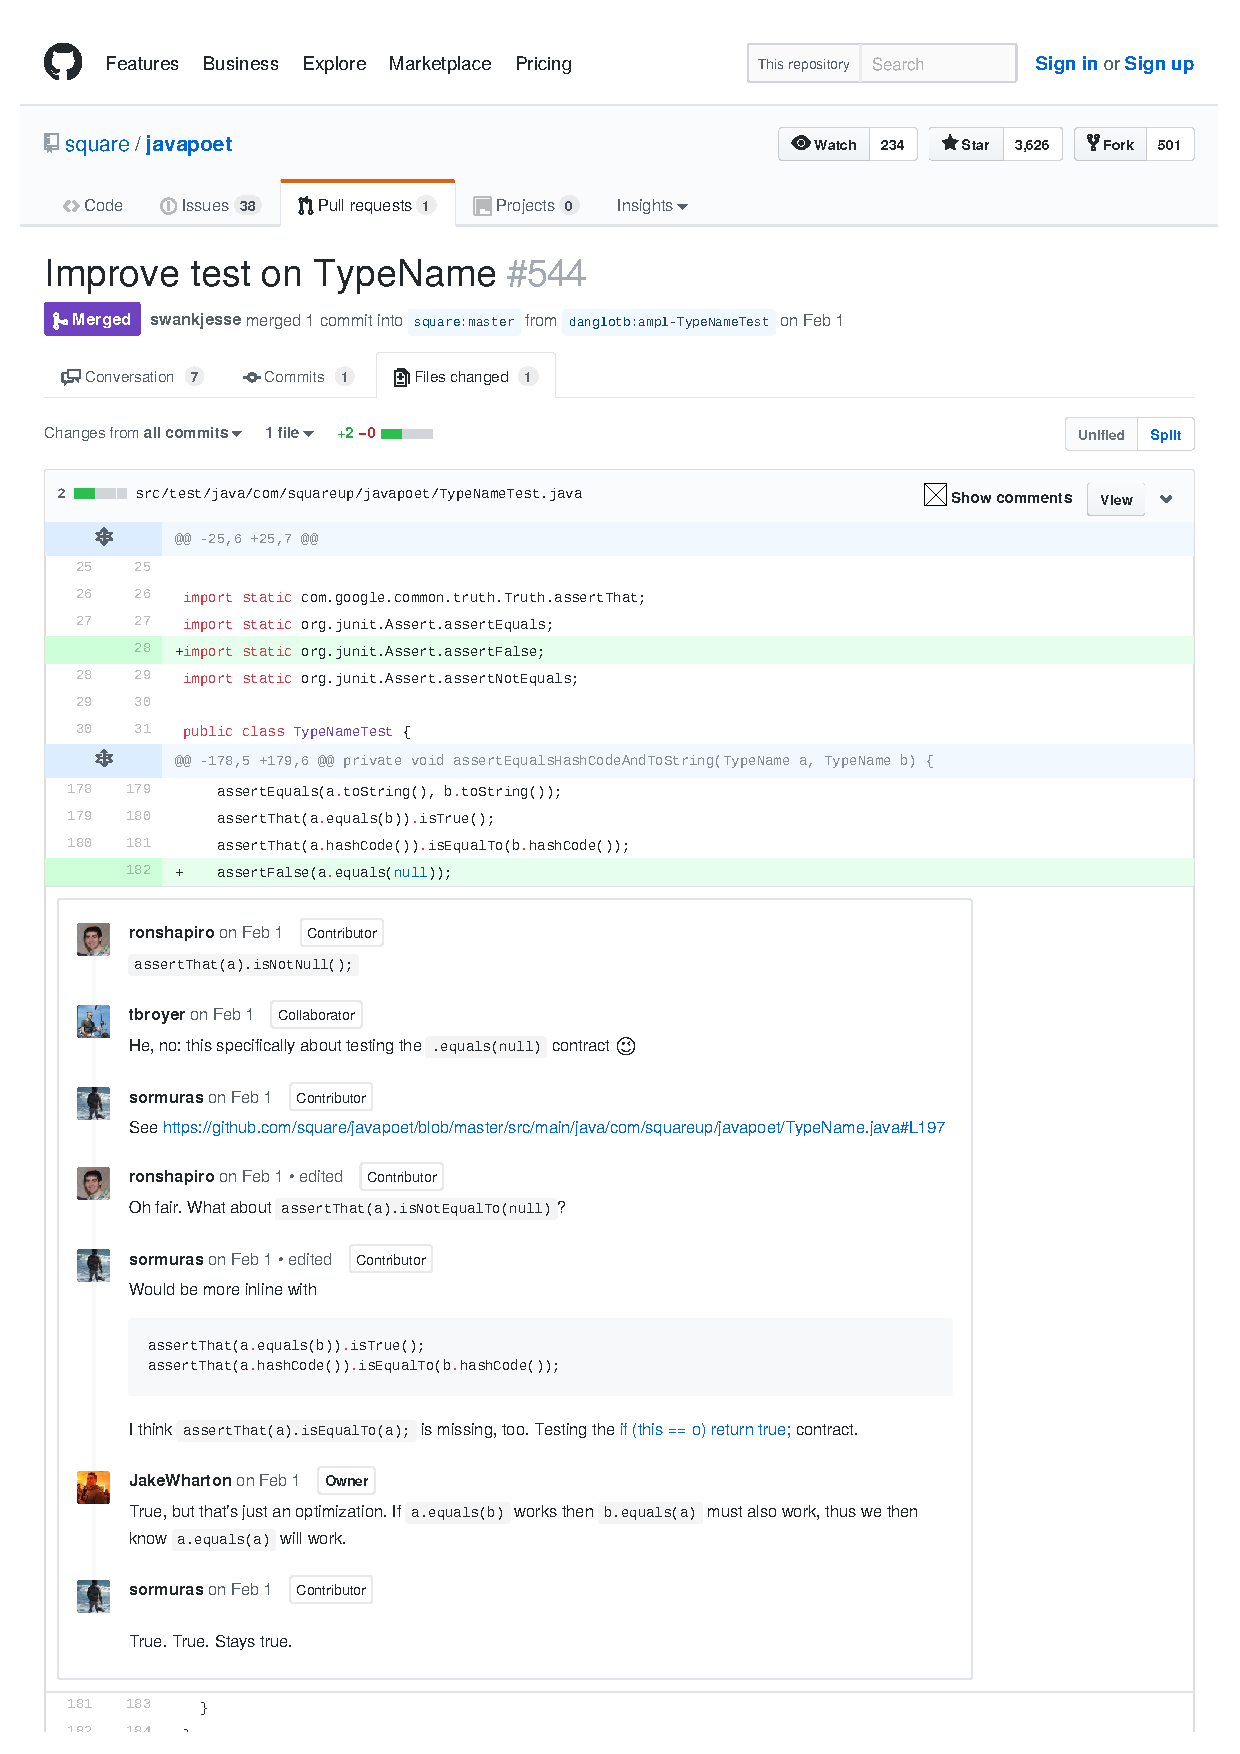
\includegraphics[width=0.98\textwidth, trim=2cm 14.4cm 10.06cm 14.0cm, clip]{javapoet.pdf}}
\end{figure}
The title of the pull resuest is: ``\emph{Improve test on TypeName}'' with the following short text: ``\emph{Hello, I open this pull request to specify the line 197 in the equals() method of com.squareup.javapoet.TypeName. if (o == null) return false;}''
This test improvement synthesized by \dspot has been merged by of the lead developer of javapoet one hour after its proposal.


% -----------------------------------------------------------------------------
% MYBATIS
% -----------------------------------------------------------------------------
\subsubsection{mybatis-3}

% mybatis-3 used: shouldGetAndSetNestedProperty_cf114673
%\todo{MyBatis is a object relational mapper framework (aka ORM). The original test suite kills 75.3\% --- 14821 over 19685 of the mutant generated by \pitest. DATASET}

In project mybatis-3, \dspot has been applied to amplify a test for \texttt{MetaClass}. 
\dspot synthesizes a single assertion that kills 8 more mutants.
All new mutants killed are located between lines 174 and 179, \ie the \texttt{then} branch of an \texttt{if-statement} in method \texttt{buildProperty(String property, StringBuilder sb)} of \texttt{MetaClass}.
This method builds a String that represents the  property given as input. 
The \texttt{then} branch is responsible to build the String in case the \texttt{property} has a child, \eg the input is ``richType.richProperty''. 
This behavior is not specified at all in the original test class.

I have proposed to the developers the following pull request entitled ``\emph{Improve test on MetaClass}'' with the following short text: ``\emph{Hello, I open this pull request to specify the lines 174-179 in the buildProperty(String, StringBuilder) method of MetaClass.}'' \footnote{\url{https://github.com/mybatis/mybatis-3/pull/912/files}}:
\begin{figure}[H]
	\centering\fbox{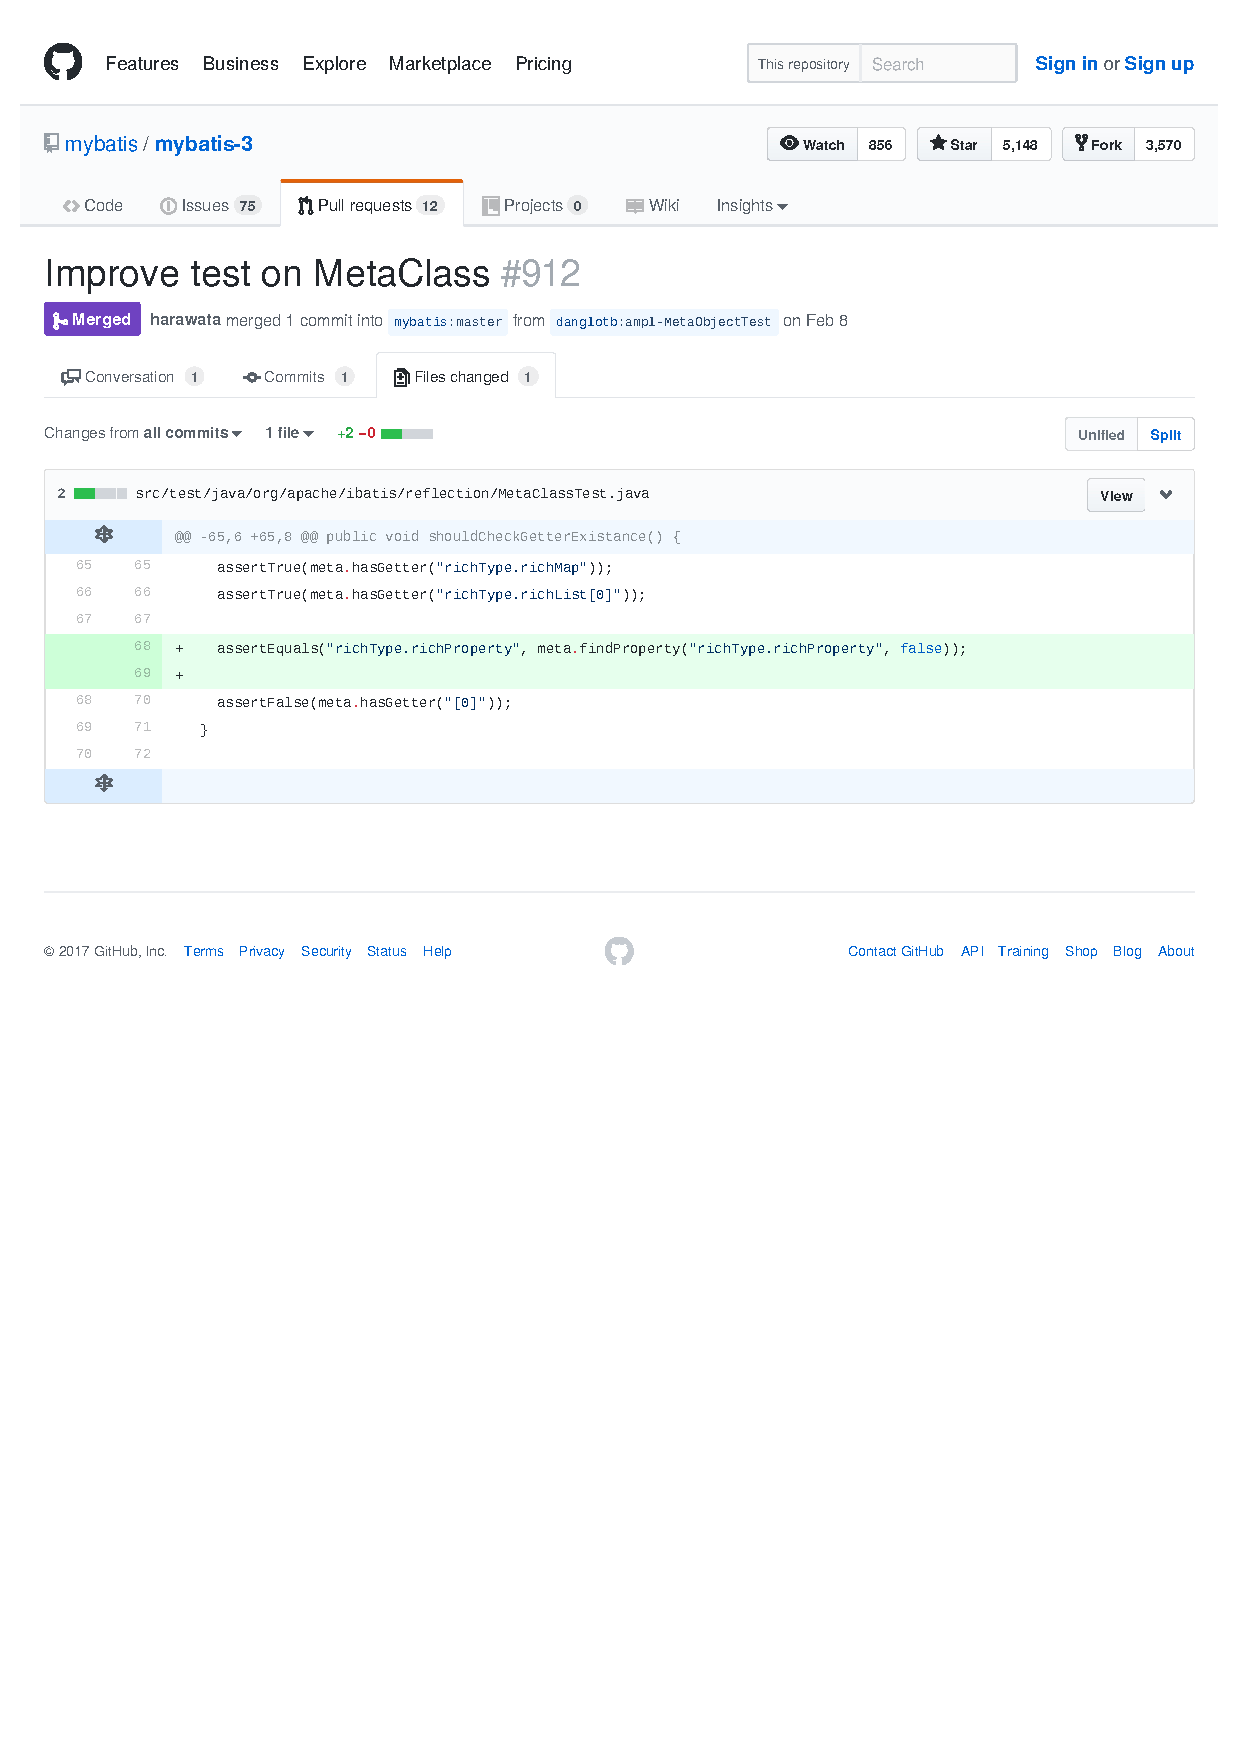
\includegraphics[width=0.98\textwidth, trim=2cm 17.5cm 4.5cm 10.5cm, clip]{mybatis.pdf}}
\end{figure}

The developer accepted the test improvement and merged the pull request the same day without a single objection. 


% -----------------------------------------------------------------------------
% TRACCAR
% -----------------------------------------------------------------------------
\subsubsection{traccar}
% top killer : testDecode_cf39

\dspot has been applied to amplify \texttt{ObdDecoderTest}. 
It identifies a single assertion that kills 14 more mutants.
All newly killed mutants are located between lines 60 to 80, \ie in the method \texttt{decodesCodes()} of \texttt{ObdDecoder}, which is responsible to decode a \texttt{String}. 
In this case, the pull request consists of a new test method because the new assertions do not fit with the intent of existing tests. 
This new test method is proposed into \texttt{ObdDecoderTest}, which is the class under amplification. 
The PR was entitled ``\emph{Improve test cases on ObdDecoder}'' with the following description: ``\emph{Hello, I open this pull request to specify the method decodeCodes of the ObdDecoder}''. \footnote{\url{https://github.com/tananaev/traccar/pull/2897}}
\begin{figure}[H]
	\centering\fbox{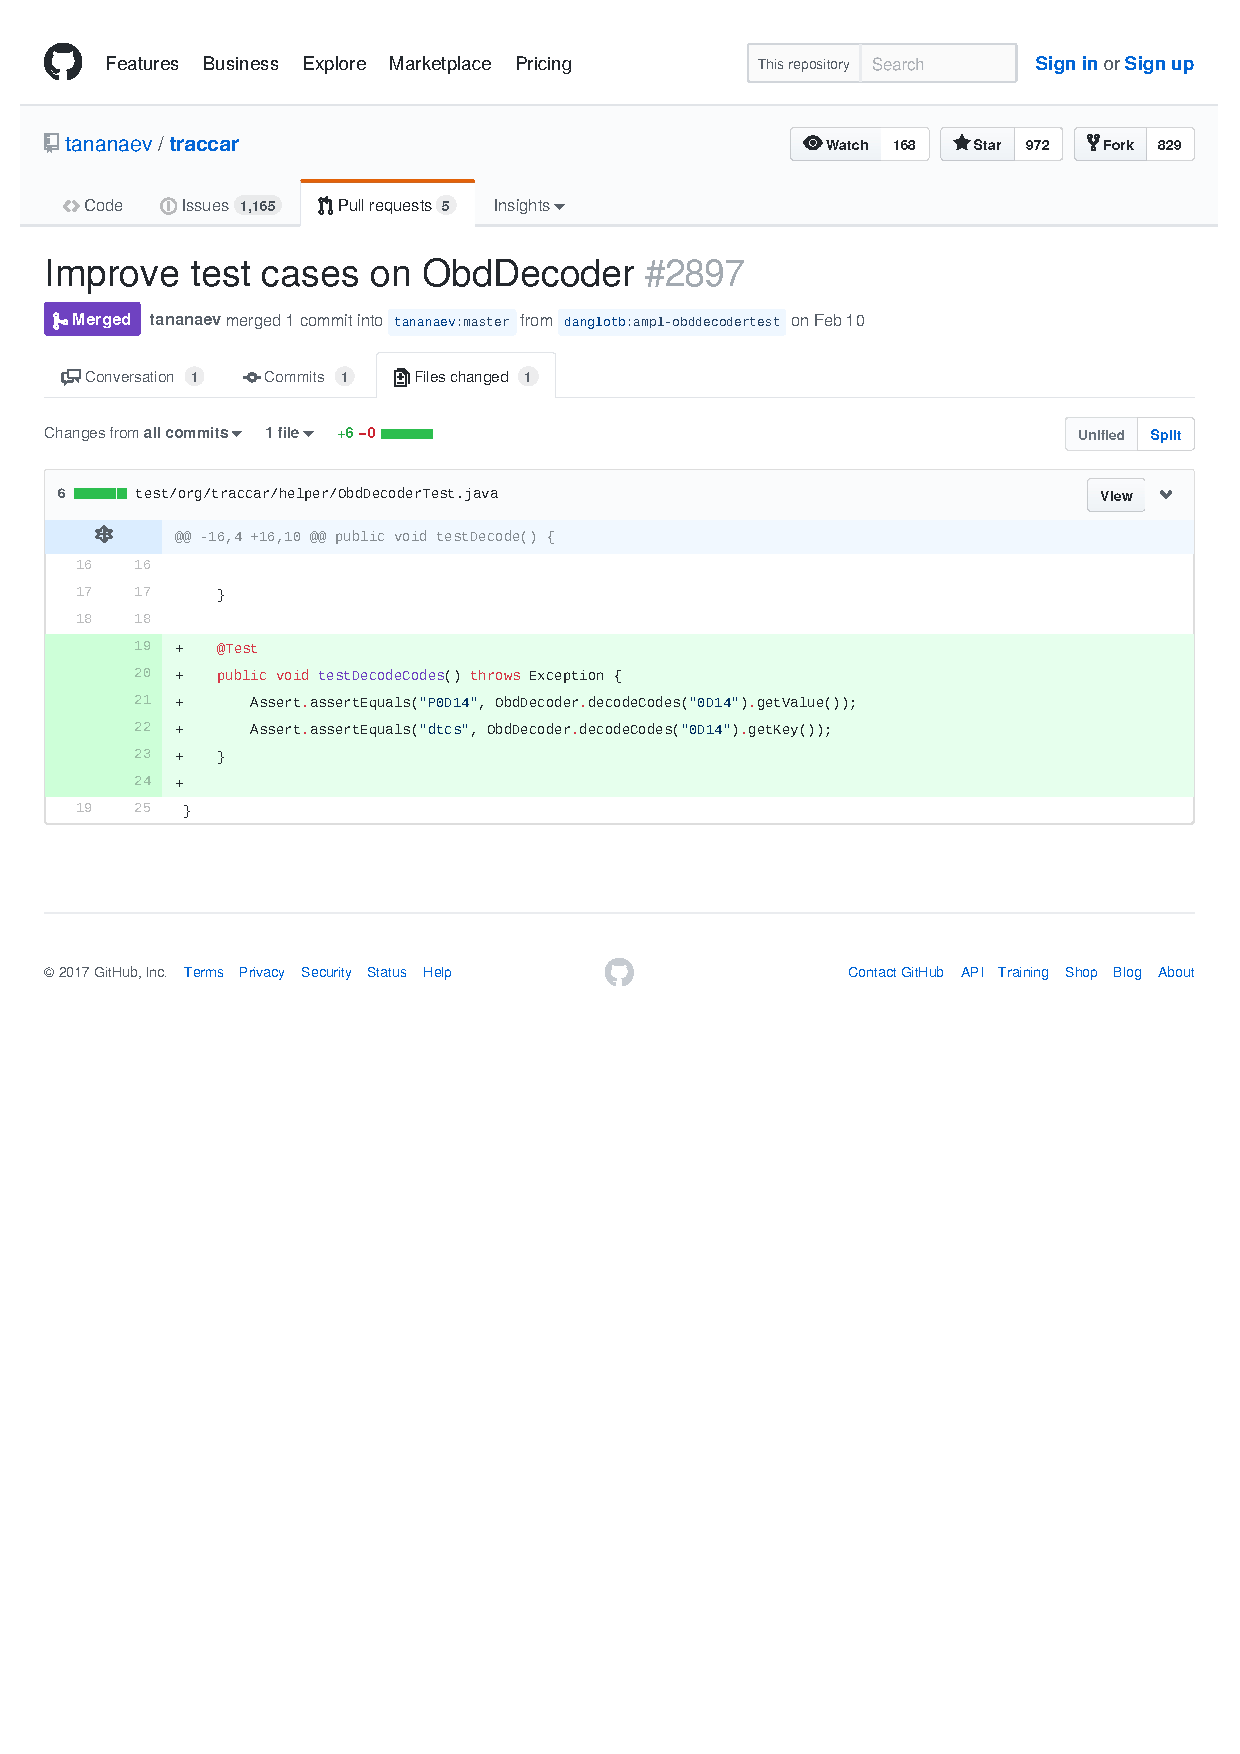
\includegraphics[width=0.98\textwidth, trim=2cm 15.57cm 6.35cm 9.88cm, clip]{traccar.pdf}}
\end{figure}

The developer of traccar thanked us for the proposed changes and merged it the same day.


% -----------------------------------------------------------------------------
% STREAM LIB
% -----------------------------------------------------------------------------
\subsubsection{stream-lib}

%testHash64ByteArrayOverload_cf92

% https://github.com/addthis/stream-lib/pull/128/files

\dspot has been applied to amplify \texttt{TestMurmurHash}. 
It identifies a new test input that kills 15 more mutants.
All newly killed mutants are located in method \texttt{hash64()} of \texttt{MurmurHash} from lines 158 to 216.
This method computes a hash for a given array of byte. 
The PR was entitled ``\emph{Test: Specify hash64}'' with the following description: ``\emph{The proposed change specifies what the good hash code must be. With the current test, any change in "hash" would still make the test pass, incl. the changes that would result in an inefficient hash.}''. \footnote{\url{https://github.com/addthis/stream-lib/pull/127/files}}:
\begin{figure}[H]
	\centering\fbox{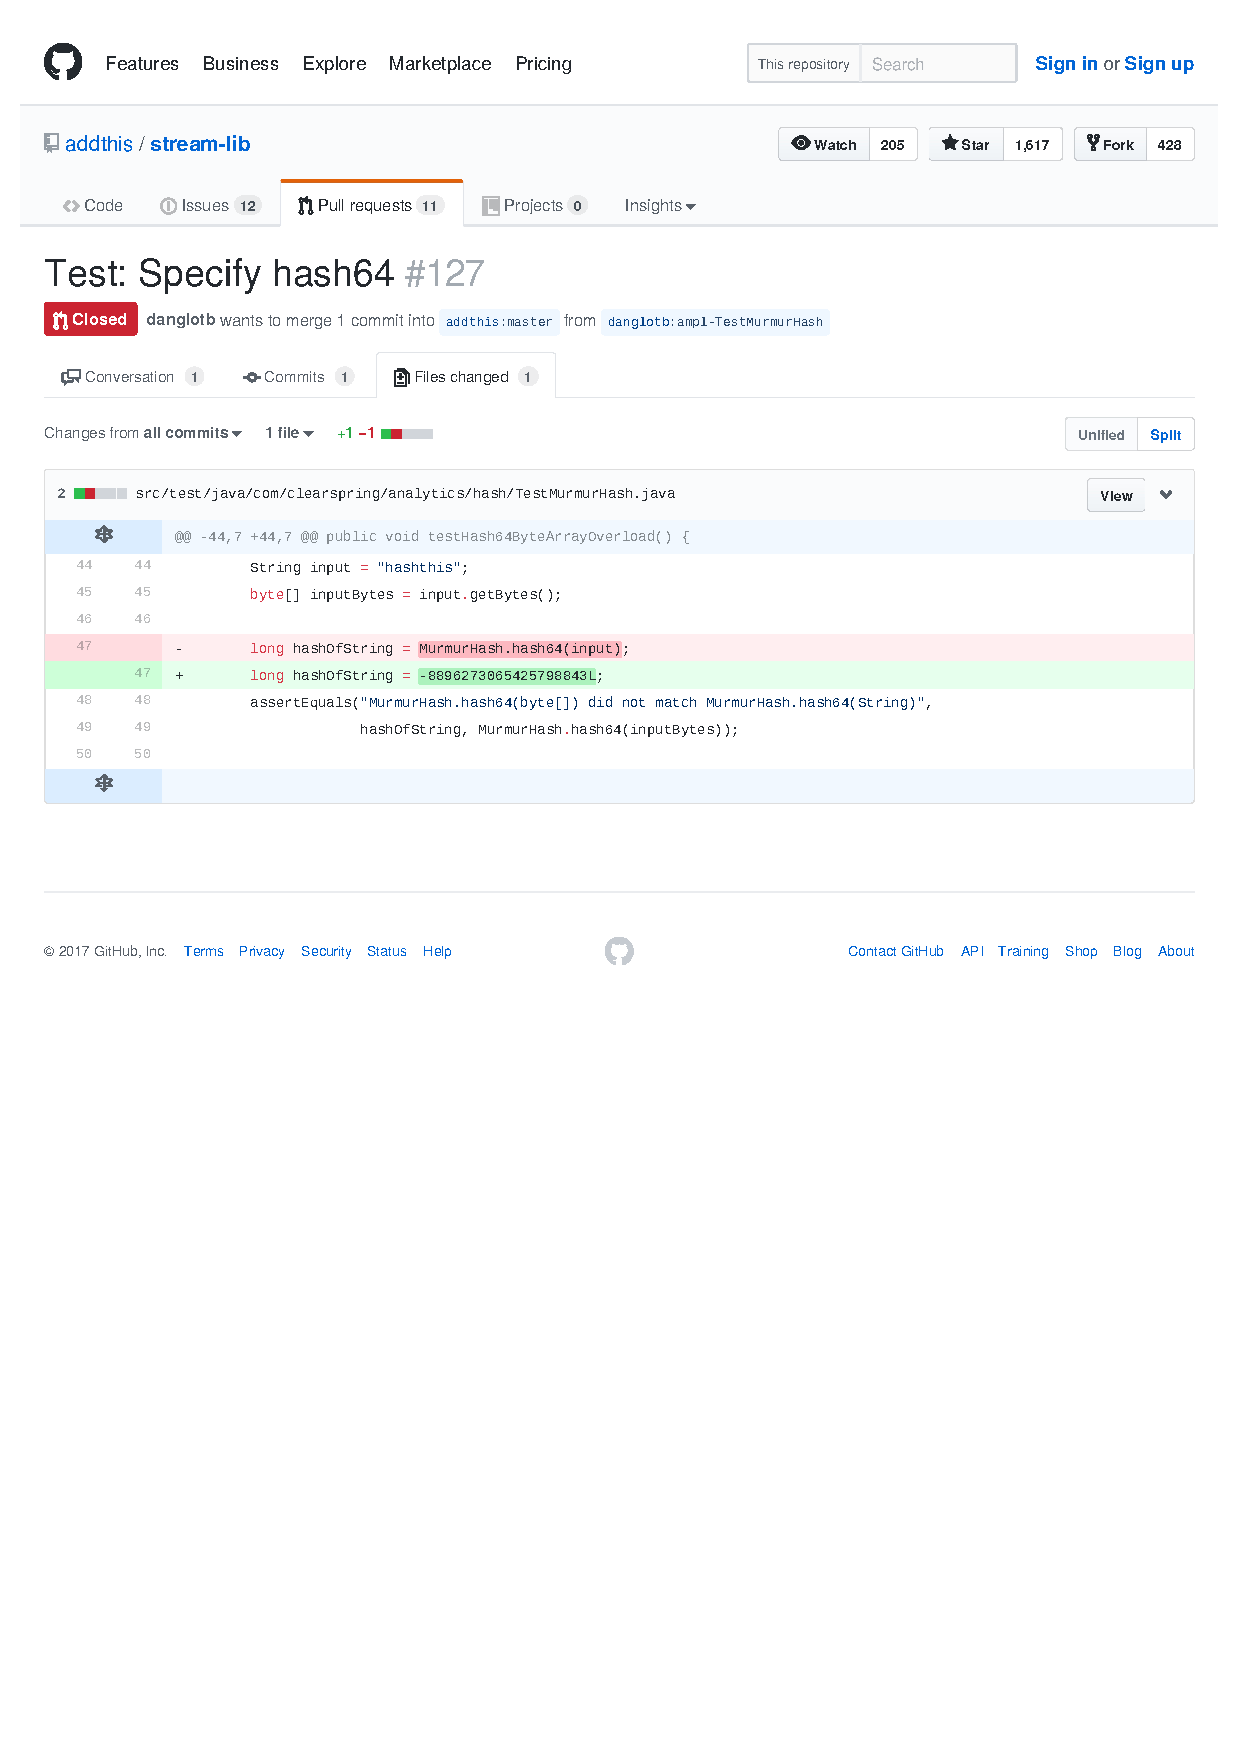
\includegraphics[width=0.98\textwidth, trim=2cm 17.07cm 4.90cm 10.59cm, clip]{stream-lib0.pdf}}
\end{figure}

Two days later, one developer mentioned the fact that the test is verifying the overload of the method and is not specifying the method hash itself. 
He closed the PR because it was not relevant to put changes there. 
He suggested to open an new pull request with a new test method instead of changing the existing test method. 
I proposed, 6 days later, a second pull request entitled ``\emph{add test for hash() and hash64() against hard coded values}'' with no description, since I estimated that the developer was aware of the test intention.\footnote{\url{https://github.com/addthis/stream-lib/pull/128/files}}:
\begin{figure}[H]
	\centering\fbox{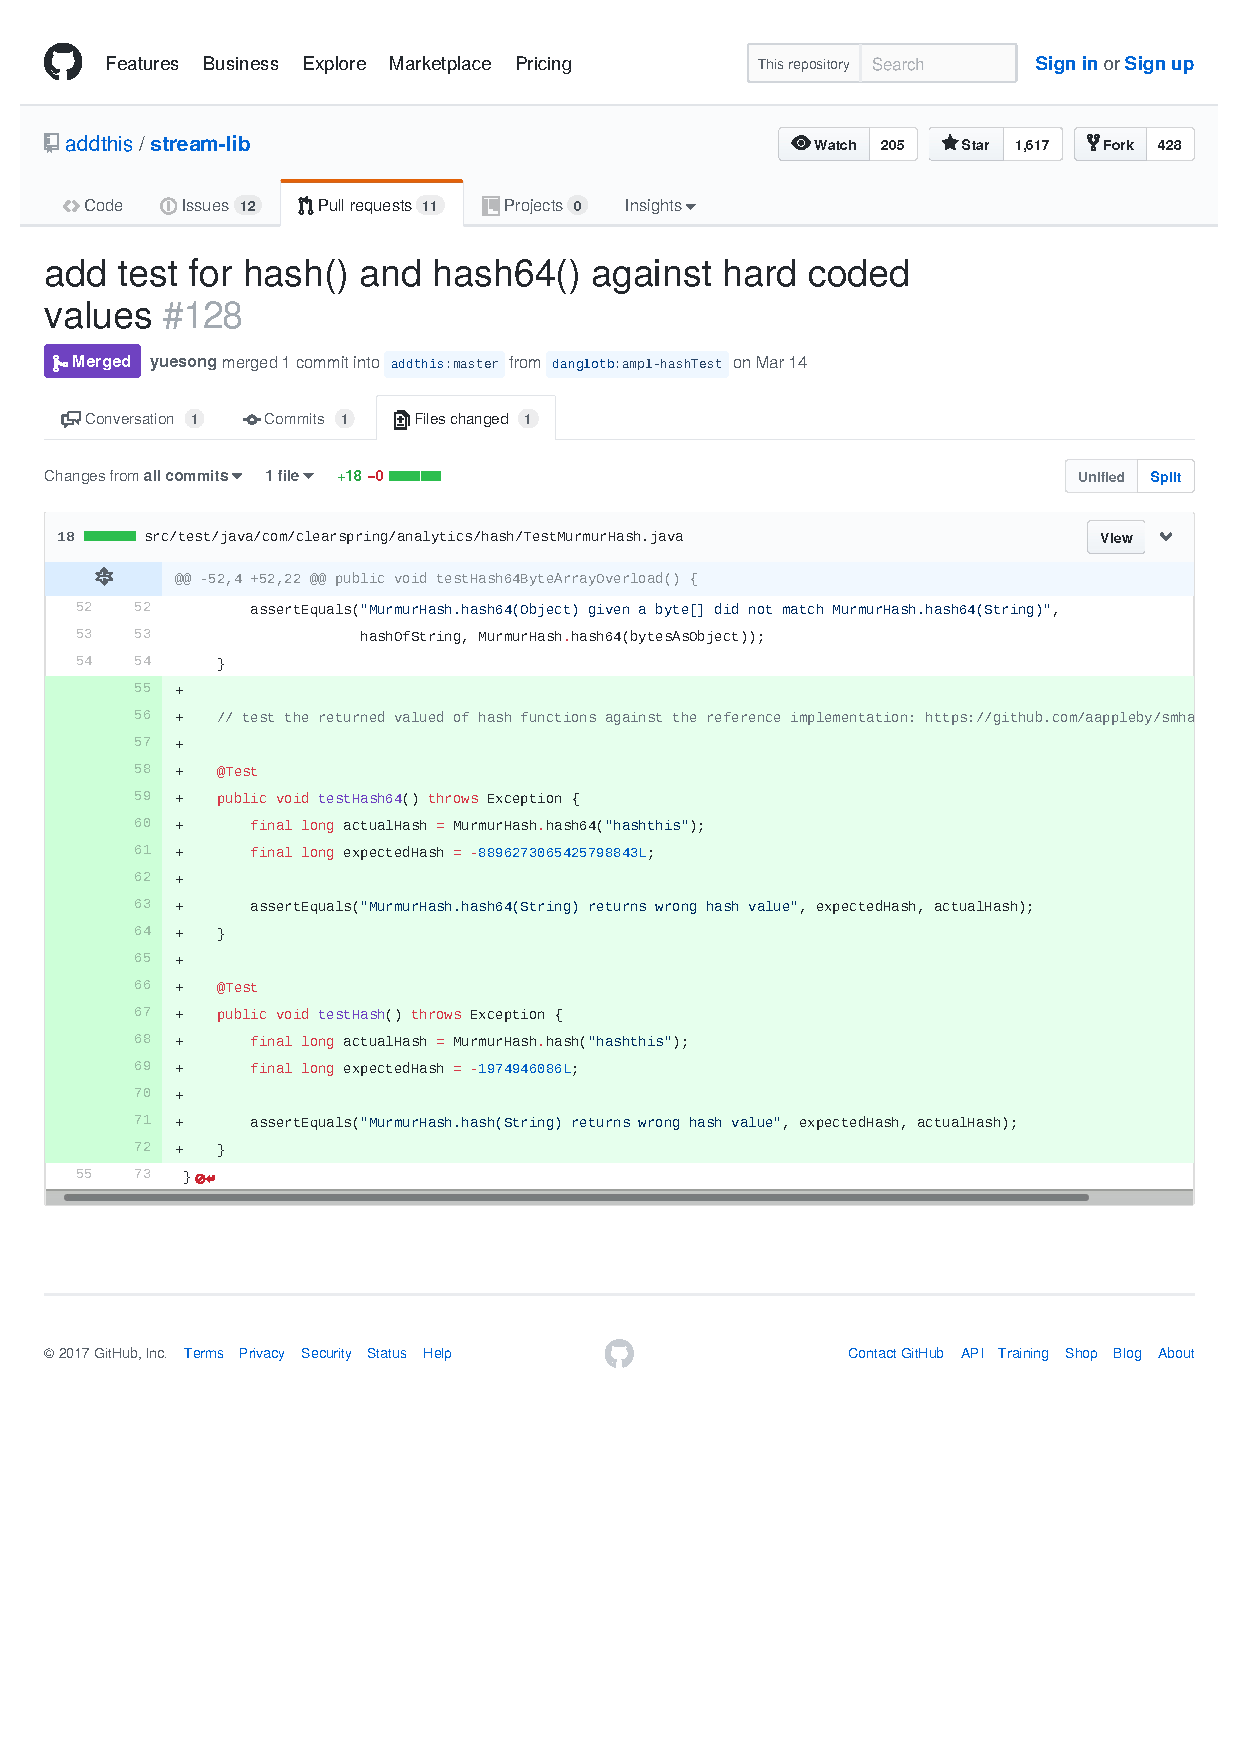
\includegraphics[width=0.98\textwidth, trim=2cm 9.55cm 3.35cm 11.02cm, clip]{stream-lib.pdf}}
\end{figure}

The pull request has been merged by the same developer 20 days later.


% -----------------------------------------------------------------------------
% MUSTACHE.JAVA
% -----------------------------------------------------------------------------
\subsubsection{mustache.java}

%testAbstractClass_add3_literalMutation38_literalMutation326_failAssert19

\dspot has been applied to amplify \texttt{AbstractClassTest}. 
It identifies a try/catch/fail block that kills 2 more mutants.
This is an interesting new case, compared to the ones previously discussed, because it is about the specification of exceptions, \ie of behavior under erroneous inputs.
All newly killed mutants are located in method \texttt{compile()} on line 194.
The test specifies that if a variable is improperly closed, the program must throw a \texttt{MustacheException}. 
In the Mustache template language, an improperly closed variable occurs when an opening brace ``$\{$'' does not have its matching closing brace such as in the input of the proposed changes. 
I propose the pull request to the developers, entitled ``\emph{Add Test: improperly closed variable}'' with the following description: ``\emph{Hello, I proposed this change to improve the test on MustacheParser. When a variable is improperly closed, a MustacheException is thrown.}''.\footnote{\url{https://github.com/spullara/mustache.java/pull/186/files}}
\begin{figure}[H]
	\centering\fbox{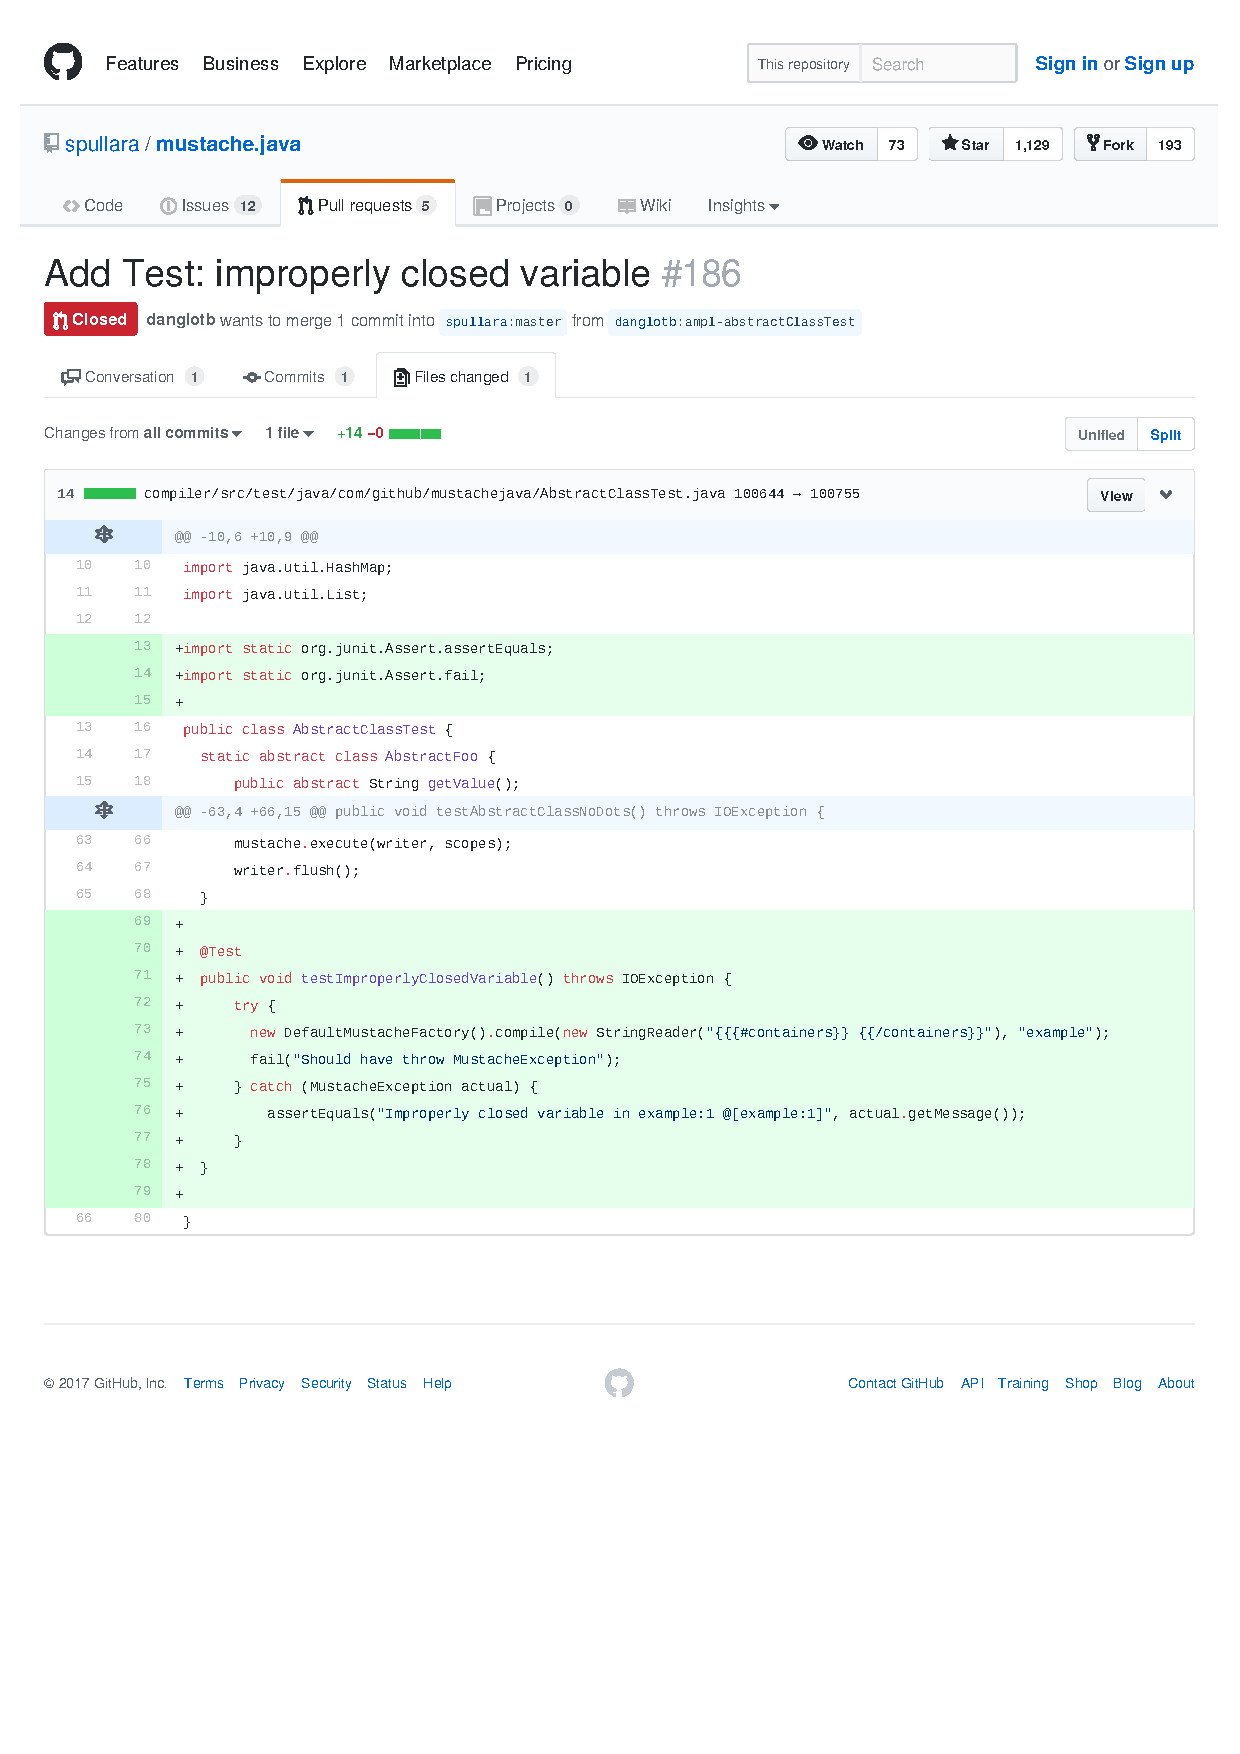
\includegraphics[width=0.98\textwidth, trim=2cm 8.86cm 2.03cm 14.96cm, clip]{mustache-java.pdf}}
\end{figure}

12 days later, a developer accepted the change, but noted that the test should be in another class.
He closed the pull request and added the changes himself into the desired class.\footnote{the diff is same:\url{https://github.com/spullara/mustache.java/commit/9efa19d595f893527ff218683e70db2ae4d8fb2d}}. 

% -----------------------------------------------------------------------------
% TWILIO-JAVA
% -----------------------------------------------------------------------------
\subsubsection{twilio-java}

\dspot has been applied to amplify \texttt{RequestTest}. 
It identifies two new assertions that kill 4 more mutants. 
All killed mutants are between lines 260 and 265 in the method \texttt{equals()} of \texttt{Request}. 
The change specifies that an object \texttt{Request} is not equal to null nor an object of different type, \ie \texttt{Object} here. 
The pull request was entitled ``\emph{add test equals() on request}'', accompanied with the short description ``\emph{Hi, I propose this change to specify the equals() method of com.twilio.http.Request, against object and null value}'' \footnote{\url{https://github.com/twilio/twilio-java/pull/334/files}}:
\begin{figure}[H]
	\centering\fbox{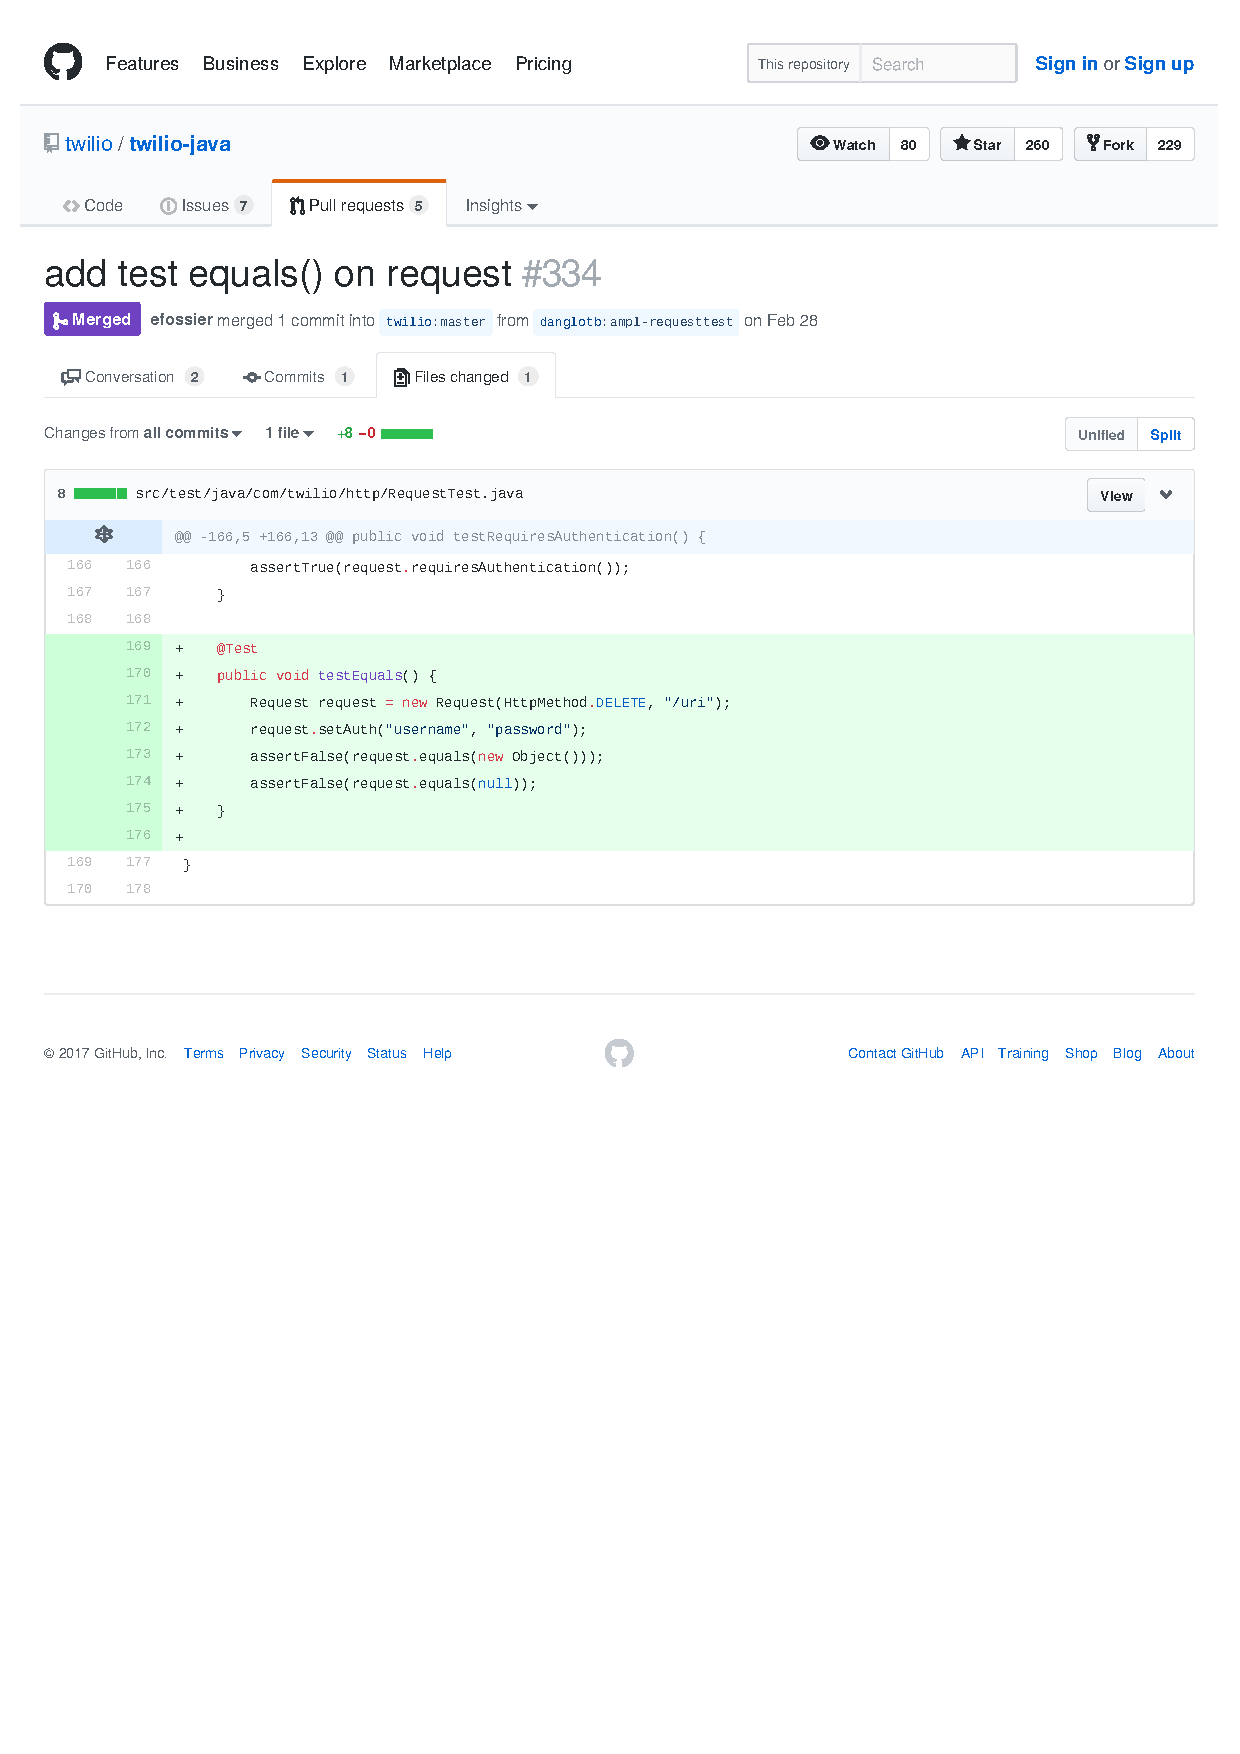
\includegraphics[width=0.98\textwidth, trim=2cm 14.83cm 8.11cm 10.11cm, clip]{twilio-java.pdf}}
\end{figure}

A developer merged the change 4 days later.

% 
% 25 minutes
% testGetUsername_cf47548_cf49619_cf53871
% best fitness, all mutant are killed in equals pr easy to build
% adding assertion manually against null, for having a complete test case.

% ExcludedClasses = com.twilio.http.NetworkHttpClientTest

% -----------------------------------------------------------------------------
% JSOUP
% -----------------------------------------------------------------------------
\subsubsection{jsoup}

\dspot has been applied to amplify \texttt{AttributeTest}. 
It identifies one assertion that kills 13 more mutants.
All mutants are in the method \texttt{hashcode} of Attribute. 
The pull request was entitled ``\emph{add test case for hashcode in attribute}'' with the following short description ``\emph{Hello, I propose this change to specify the hashCode of the object org.jsoup.nodes.Attribute.}''\footnote{\url{https://github.com/jhy/jsoup/pull/840}}:
\begin{figure}[H]
	\centering\fbox{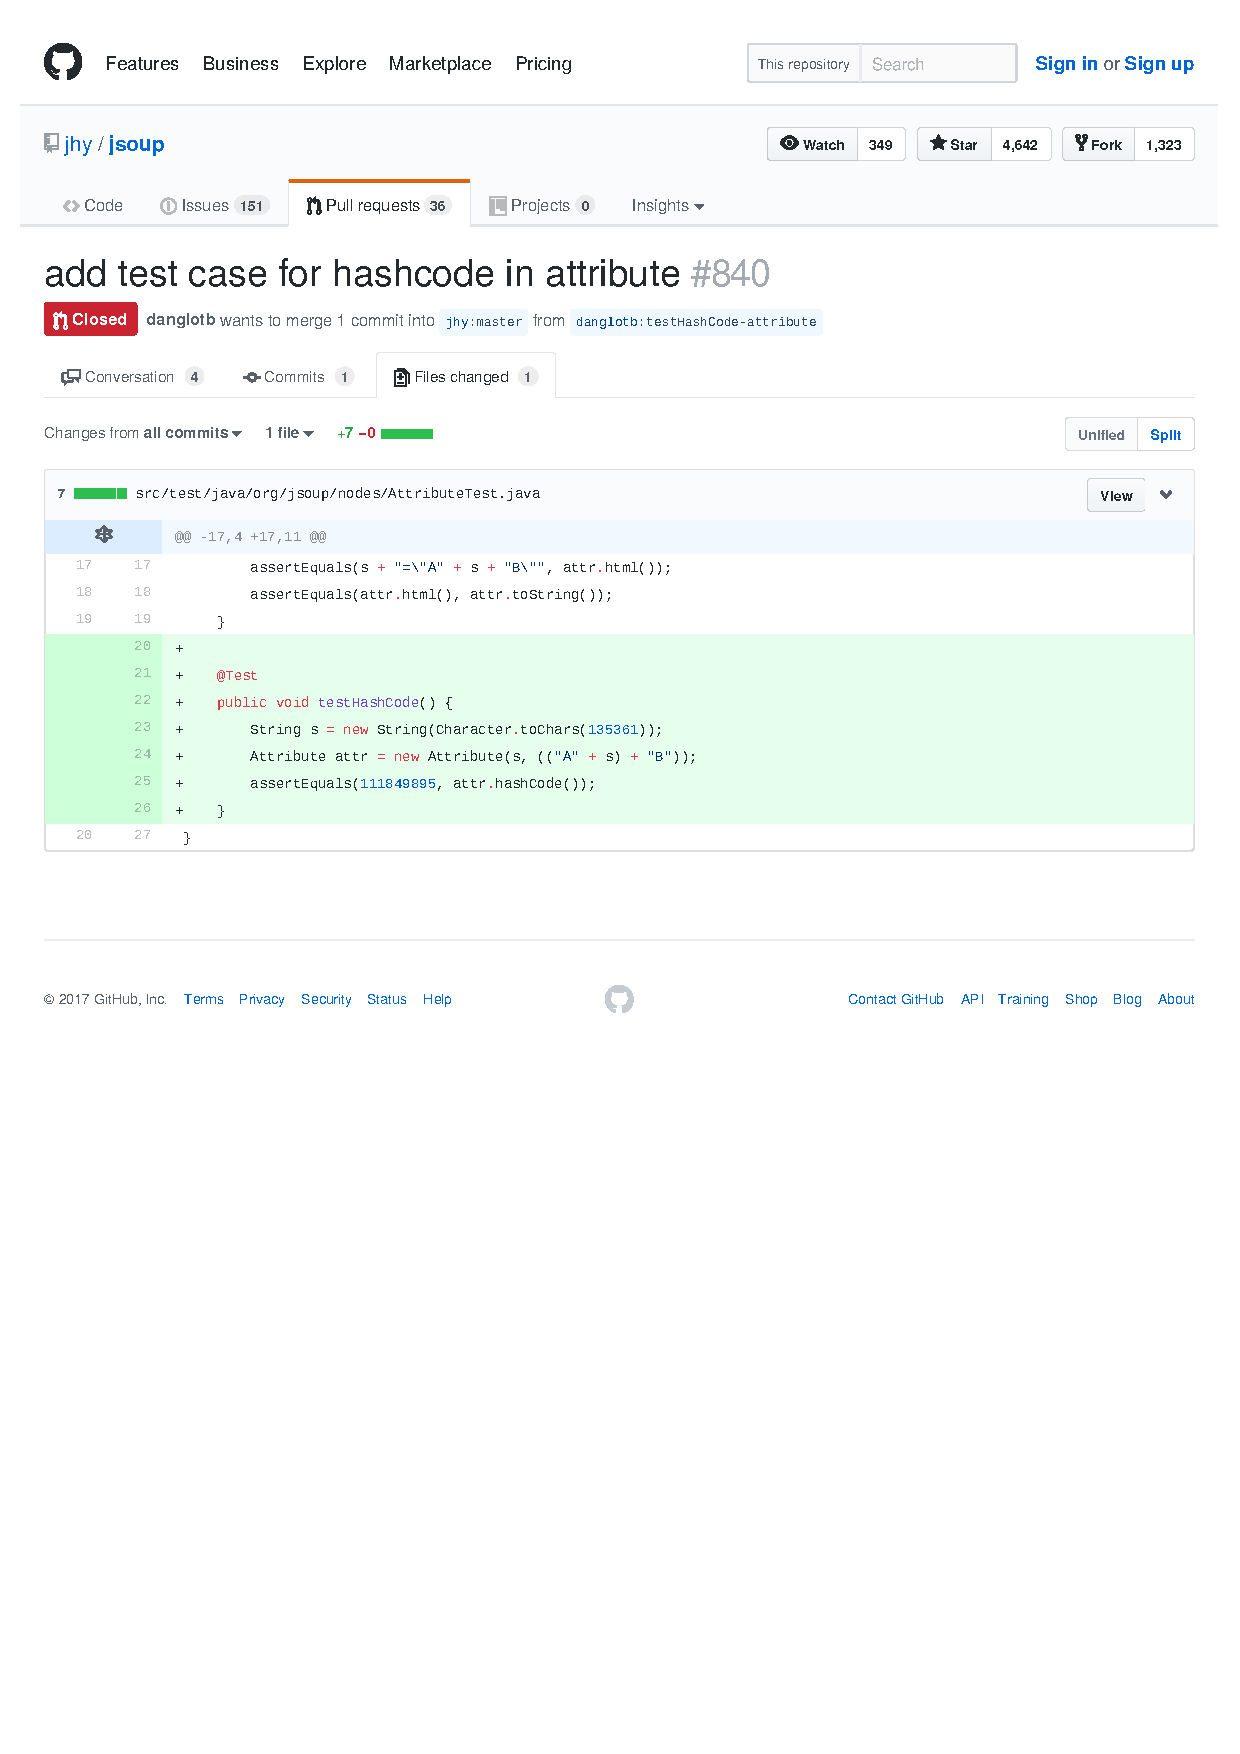
\includegraphics[width=0.98\textwidth, trim=2cm 15.5cm 9cm 10.4cm, clip]{jsoup.pdf}}
\end{figure}

One developer highlighted the point that the \texttt{hashCode} method is an implementation detail, and it is not a relevant element of the API. 
Consequently, he did not accept our test improvement.

At this point, I have made two pull requests targeting \texttt{hashCode} methods. 
One accepted and one rejected. 
\texttt{hashCode} methods could require a different testing approach to validate the number of potential collisions in a collection of objects rather than checking or comparing the values of a few objects created for one explicit test case.
The different responses obtained reflect the fact that developer teams and policies ultimately decide how to test the hash code protocol and the outcome could be different from different projects.

%\TODO{I don't know if i disagree with this developer now, because the contract should be tested not the values.}s
%We disagree with this developer, and think that \texttt{hashCode} methods are worth a test case, because the contracts of \texttt{hashCode} methods are essential for many high-level usages such as collection usages. However, we would agree that such generic test cases may be generated by a dedicated testing framework.


% -----------------------------------------------------------------------------
% PROTOSTUFF
% -----------------------------------------------------------------------------
\subsubsection{protostuff}

\dspot has been applied to amplify \texttt{TailDelimiterTest}. 
It identifies a single assertion that kills 3 more mutants.
All new mutants killed are in the method \texttt{writeTo} of \texttt{ProtostuffIOUtil} on lines 285 and 286, which is responsible to write a buffer into a given scheme. 
I proposed a pull request entitled ``\emph{assert the returned value of writeList}'', with the following short description ``\emph{Hi, I propose the following changes to specify the line 285-286 of io.protostuff.ProtostuffIOUtil.}''\footnote{\url{https://github.com/protostuff/protostuff/pull/212/files}}, shown earlier in \autoref{fig:diff-protostuff}

\begin{figure}[H]
	\centering\fbox{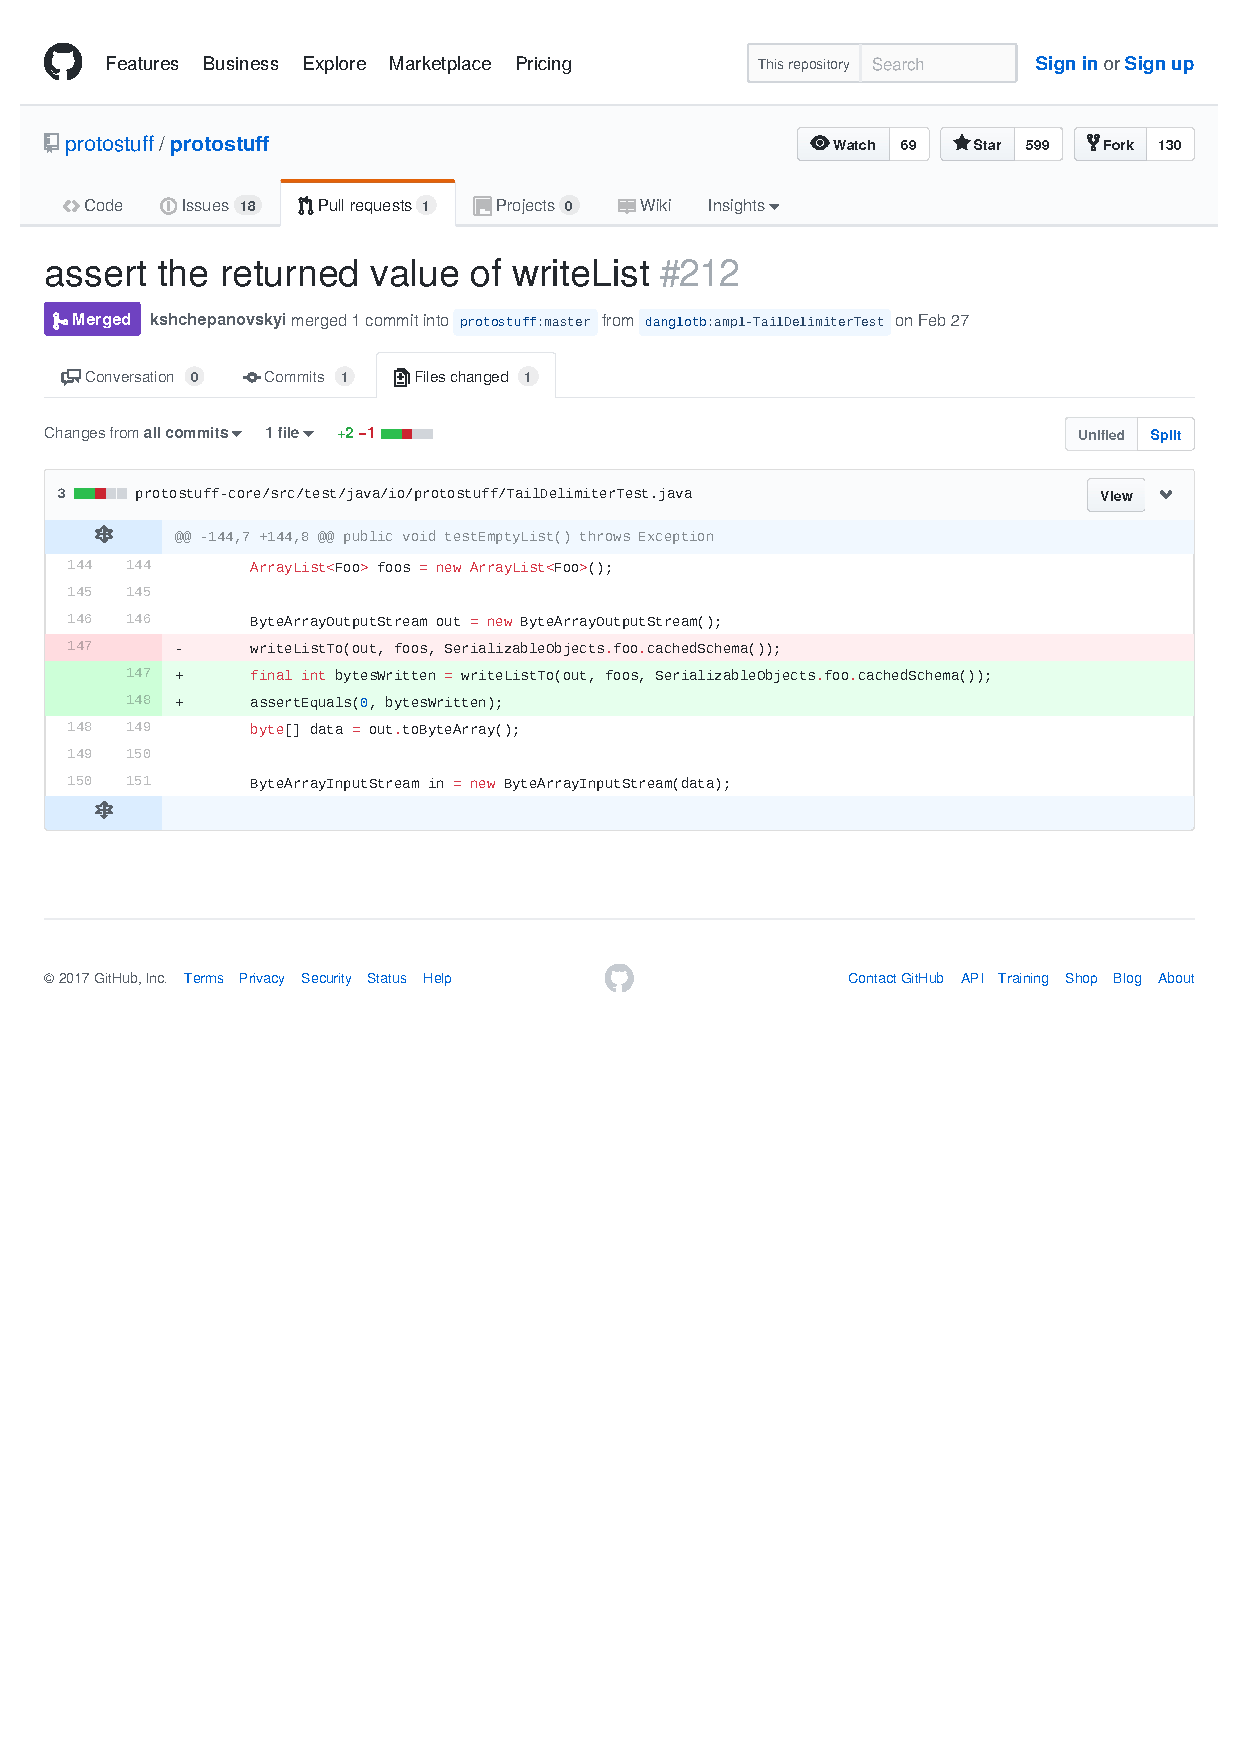
\includegraphics[width=0.98\textwidth, trim=2cm 16.3cm 4cm 10.4cm, clip]{protostuff.pdf}}
\end{figure}

A developer accepted the proposed changes the same day.

%testEmptyList_add5651

% -----------------------------------------------------------------------------
% LOGBACK
% -----------------------------------------------------------------------------
\subsubsection{logback}

\dspot has been applied to amplify \texttt{FileNamePattern}. 
It identifies a single assertion that kills 5 more mutant. 
Newly killed mutants were located at lines 94, 96 and 97 of the \texttt{equals} method of the \texttt{FileNamePattern} class. 
The proposed pull request was entitle ``\emph{test: add test on equals of FileNamePattern against null value}'' with the following short description: ``\emph{Hello, I propose this change to specify the equals() method ofFileNamePattern against null value}''.\footnote{\url{https://github.com/qos-ch/logback/pull/365/files}}:

\begin{figure}[H]
	\centering\fbox{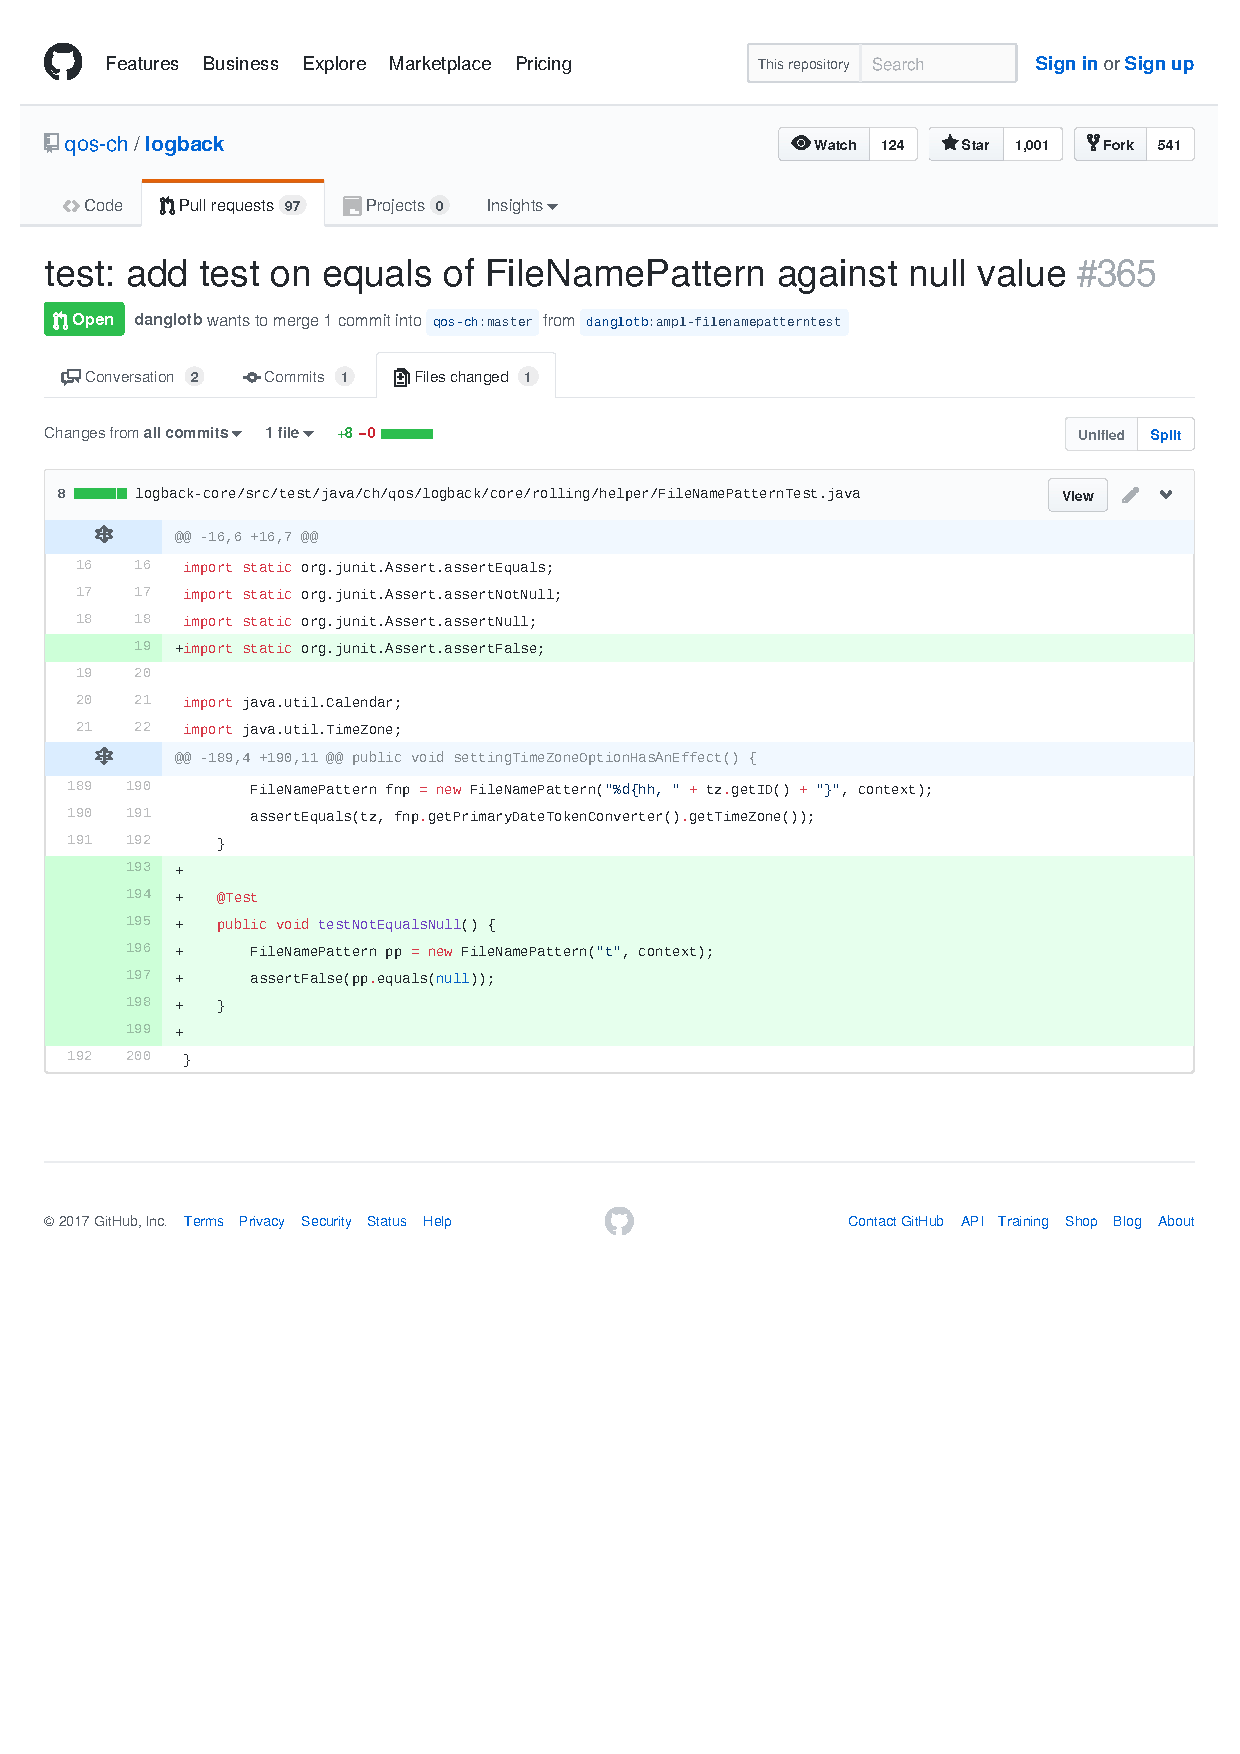
\includegraphics[width=0.98\textwidth, trim=2cm 11.66cm 8.69cm 14.20cm, clip]{logback.pdf}}
\end{figure}

Even if the test asserts the contract that the \texttt{FileNamePattern} is not equals to null, and kills 5 more mutants, the lead developer does not get the point to test this behavior. 
The pull request has not been accepted.

%testSmoke_cf69003

% -----------------------------------------------------------------------------
% RETROFIT
% -----------------------------------------------------------------------------
\subsubsection{retrofit}

I did not manage to create a pull request based on the amplification of the test suite of retrofit. 
According to the result, the newly killed mutants are spread over all the code, and thus the amplified methods did not identify a missing contract specification. 
This could be explained by two facts: 
1) the original test suite of retrofit is strong: there is no test class with low \ms and a lot of them are very high \ms, \ie 90\% and more;
2) the original test suite of retrofit uses complex test mechanism such as mock and fluent assertions of the form the \texttt{assertThat().isSomething()}. 
For the former point, it means that \dspot has been able to improve, even a bit, the \ms of a very strong test suite, but not in targeted way that makes sense in a pull request.
For the latter point, this puts in evidence the technical challenge of amplifying fluent assertions and mocking mechanisms.

\subsubsection{Contributions of \Aampl and \Iampl to the Pull-requests}

\begin{table}[]
	\caption{Contributions of \Aampl and \Iampl on the amplified test method used to create a pull request.}
	\label{tab:contrib-a-i-ampl}
	\centering\begin{tabular}{lcc}
		\hline
		Project & \#\Aampl &  \#\Iampl \\
		\hline
		javapoet & 2 & 2 \\
		mybatis-3 & 3 & 3 \\
		traccar & 10 & 7 \\
		stream-lib & 2 & 2 \\
		mustache & 4 & 3 \\
		twilio & 3 & 4 \\
		jsoup & 34 & 0 \\
		protostuff & 1 & 1 \\
		logback & 2 & 2 \\
		\hline
	\end{tabular}
\end{table}

\autoref{tab:contrib-a-i-ampl} summarizes the contribution of \Aampl and \Iampl, where a contribution means an source code modification added during the main amplification loop. 
In 8 cases over the 9 pull-requests, both \Aampl and \Iampl were necessary. 
Only the pull request on jsoup was found using only \Aampl. 
This means that for all the other pull-requests, the new inputs were required to be able: 
1) to kill new mutants and 
2) to obtain amplified test methods that have values for the developers.

Note that this does not contradict with the fact that the pull requests are one-liners.
Most one-liner pull requests contain both a new assertion and a new input. Consider the following Javapoet's one liner \texttt{assertFalse(x.equals(null))} (javapoet). 
In this example, although there is a single line starting with ``assert'', there is indeed a new input, the value ``null''.

~\\
~\\
\begin{mdframed}
	\textit{\rqpullrequest: Would developers be ready to permanently accept improved test cases into the test repository?}\\
	Answer: 19 test improvements have been proposed to developers of notable open-source projects. 
	13/19 have been considered valuable and have been merged into the main test suite. 
	The developers' feedback has confirmed the relevance, and also the challenges of automated test improvement.
\end{mdframed}

In the area of automatic test improvement, this experiment is the first to put real developers in the loop, by asking them about the quality of automatically improved test cases.
To the best of my knowledge, this is the first public report of automatically improved tests accepted by unbiased developers and merged in the master branch of open-source repositories.

\begin{table}
	\caption{The effectiveness of test amplification with \dspot on 40 test classes: 24 well-tested (upper part) and 16 average-tested (lower part) real test classes from notable open-source Java projects.}
	%A star after a test name means that the test is considered as subject for the relevance study of \rqpullrequest.}
	\label{tab:overall-results}
	\def\arraystretch{0.55}%  1 is the default, change whatever you need
	\setlength\tabcolsep{0.45pt} % default value: 6pt
	\small
	\begin{tabular}{|llrrrr|rrrr|rrr|r|}
		\rotverticalinv{ID}&
		\rotverticalinv{Class}&
		\rotverticalinv{\# Orig. test methods}&
		\rotverticalinv{Mutation Score}&
		\rotverticalinv{\# New test methods}&
		\rotverticalinv{\begin{tabular}{l}
				Candidates \\ for pull request
		\end{tabular}}&
		\rotverticalinv{\# Killed mutants orig.}&
		\rotverticalinv{\# Killed mutants ampl.}&
		\rotverticalinv{Increase killed}&
		&%arrow for killed
		\setlength{\tabcolsep}{0cm} 
		\rotverticalinv{\begin{tabular}{l}
				\# Killed mutants only\\ A-ampl
		\end{tabular}}&
		\setlength{\tabcolsep}{0cm} 
		\rotverticalinv{\begin{tabular}{l}
				Increase killed only\\ A-ampl
		\end{tabular}}&
		&%arrow for killed
		\rotverticalinv{Time (minutes)}\\
		\hline\\
		&\multicolumn{3}{l}{High \ms}\\
		\hline\\
		1&\scriptsize{TypeNameTest}&12&50\%&19&8&599&715&19\%&{\color{ForestGreen}$\nearrow$}&599&0.0\%&$\rightarrow$&11.11 \\
		\rowcolor[HTML]{EFEFEF}
		2&\scriptsize{NameAllocatorTest}&11&87\%&0&0&79&79&0.0\%&$\rightarrow$&79&0.0\%&$\rightarrow$&4.76 \\
		3&\scriptsize{MetaClassTest}&7&58\%&108&10&455&534&17\%&{\color{ForestGreen}$\nearrow$}&455&0.0\%&$\rightarrow$&235.71 \\
		\rowcolor[HTML]{EFEFEF}
		4&\scriptsize{ParameterExpressionTest}&14&91\%&2&2&162&164&1\%&{\color{ForestGreen}$\nearrow$}&162&0.0\%&$\rightarrow$&25.93 \\
		5&\scriptsize{ObdDecoderTest}&1&80\%&9&2&51&54&5\%&{\color{ForestGreen}$\nearrow$}&51&0.0\%&$\rightarrow$&2.20 \\
		\rowcolor[HTML]{EFEFEF}
		6&\scriptsize{MiscFormatterTest}&1&72\%&5&5&42&47&11\%&{\color{ForestGreen}$\nearrow$}&42&0.0\%&$\rightarrow$&1.21 \\
		7&\scriptsize{TestLookup3Hash}&2&95\%&0&0&464&464&0.0\%&$\rightarrow$&464&0.0\%&$\rightarrow$&6.76 \\
		\rowcolor[HTML]{EFEFEF}
		8&\scriptsize{TestDoublyLinkedList}&7&92\%&1&1&104&105&0.97\%&{\color{ForestGreen}$\nearrow$}&104&0.0\%&$\rightarrow$&3.03 \\
		9&\scriptsize{ArraysIndexesTest}&1&53\%&15&4&576&647&12\%&{\color{ForestGreen}$\nearrow$}&586&1\%&{\color{ForestGreen}$\nearrow$}&10.58 \\
		\rowcolor[HTML]{EFEFEF}
		10&\scriptsize{ClasspathResolverTest}&10&67\%&0&0&50&50&0.0\%&$\rightarrow$&50&0.0\%&$\rightarrow$&4.18 \\
		11&\scriptsize{RequestTest}&17&81\%&4&3&141&156&10\%&{\color{ForestGreen}$\nearrow$}&141&0.0\%&$\rightarrow$&60.55 \\
		\rowcolor[HTML]{EFEFEF}
		12&\scriptsize{PrefixedCollapsibleMapTest}&4&96\%&0&0&54&54&0.0\%&$\rightarrow$&54&0.0\%&$\rightarrow$&13.28 \\
		13&\scriptsize{TokenQueueTest}&6&69\%&18&6&152&165&8\%&{\color{ForestGreen}$\nearrow$}&152&0.0\%&$\rightarrow$&15.61 \\
		\rowcolor[HTML]{EFEFEF}
		14&\scriptsize{CharacterReaderTest}&19&79\%&71&9&309&336&8\%&{\color{ForestGreen}$\nearrow$}&309&0.0\%&$\rightarrow$&57.06 \\
		15&\scriptsize{TailDelimiterTest}&10&71\%&1&1&381&384&0.79\%&{\color{ForestGreen}$\nearrow$}&381&0.0\%&$\rightarrow$&12.90 \\
		\rowcolor[HTML]{EFEFEF}
		16&\scriptsize{LinkBufferTest}&3&48\%&12&7&66&90&36\%&{\color{ForestGreen}$\nearrow$}&66&0.0\%&$\rightarrow$&3.24 \\
		17&\scriptsize{FileNamePatternTest}&12&58\%&27&9&573&686&19\%&{\color{ForestGreen}$\nearrow$}&573&0.0\%&$\rightarrow$&25.08 \\
		\rowcolor[HTML]{EFEFEF}
		18&\scriptsize{SyslogAppenderBaseTest}&1&95\%&1&1&143&148&3\%&{\color{ForestGreen}$\nearrow$}&143&0.0\%&$\rightarrow$&7.88 \\
		19&\scriptsize{RequestBuilderAndroidTest}&2&99\%&0&0&513&513&0.0\%&$\rightarrow$&513&0.0\%&$\rightarrow$&0.04 \\
		\rowcolor[HTML]{EFEFEF}
		20&\scriptsize{CallAdapterTest}&4&94\%&0&0&55&55&0.0\%&$\rightarrow$&55&0.0\%&$\rightarrow$&7.30 \\
		\hline
		&\multicolumn{3}{l}{Low \ms}\\
		\hline
		21&\scriptsize{FieldSpecTest}&2&31\%&12&4&223&316&41\%&{\color{ForestGreen}$\nearrow$}&223&0.0\%&$\rightarrow$&4.44 \\
		\rowcolor[HTML]{EFEFEF}
		22&\scriptsize{ParameterSpecTest}&2&32\%&11&5&214&293&36\%&{\color{ForestGreen}$\nearrow$}&214&0.0\%&$\rightarrow$&3.66 \\
		23&\scriptsize{WrongNamespacesTest}&2&8\%&6&1&78&249&219\%&{\color{ForestGreen}$\nearrow$}&249&219\%&{\color{ForestGreen}$\nearrow$}&29.70 \\
		\rowcolor[HTML]{EFEFEF}
		24&\scriptsize{WrongMapperTest}&1&8\%&3&1&97&325&235\%&{\color{ForestGreen}$\nearrow$}&325&235\%&{\color{ForestGreen}$\nearrow$}&7.13 \\
		25&\scriptsize{ProgressProtocolDecoderTest}&1&16\%&2&1&18&27&50\%&{\color{ForestGreen}$\nearrow$}&23&27\%&{\color{ForestGreen}$\nearrow$}&1.30 \\
		\rowcolor[HTML]{EFEFEF}
		26&\scriptsize{IgnitionEventHandlerTest}&1&22\%&0&0&13&13&0.0\%&$\rightarrow$&13&0.0\%&$\rightarrow$&0.77 \\
		27&\scriptsize{TestICardinality}&2&7\%&0&0&19&19&0.0\%&$\rightarrow$&19&0.0\%&$\rightarrow$&2.13 \\
		\rowcolor[HTML]{EFEFEF}
		28&\scriptsize{TestMurmurHash}&2&17\%&40&2&52&275&428\%&{\color{ForestGreen}$\nearrow$}&174&234\%&{\color{ForestGreen}$\nearrow$}&2.18 \\
		29&\scriptsize{ConcurrencyTest}&2&28\%&2&0&210&342&62\%&{\color{ForestGreen}$\nearrow$}&210&0.0\%&$\rightarrow$&315.56 \\
		\rowcolor[HTML]{EFEFEF}
		30&\scriptsize{AbstractClassTest}&2&34\%&28&4&383&475&24\%&{\color{ForestGreen}$\nearrow$}&405&5\%&{\color{ForestGreen}$\nearrow$}&12.67 \\
		31&\scriptsize{AllTimeTest}&3&42\%&0&0&163&163&0.0\%&$\rightarrow$&163&0.0\%&$\rightarrow$&0.02 \\
		\rowcolor[HTML]{EFEFEF}
		32&\scriptsize{DailyTest}&3&42\%&0&0&163&163&0.0\%&$\rightarrow$&163&0.0\%&$\rightarrow$&0.02 \\
		33&\scriptsize{AttributeTest}&2&36\%&33&11&178&225&26\%&{\color{ForestGreen}$\nearrow$}&180&1\%&{\color{ForestGreen}$\nearrow$}&10.76 \\
		\rowcolor[HTML]{EFEFEF}
		34&\scriptsize{AttributesTest}&5&52\%&9&6&316&322&1\%&{\color{ForestGreen}$\nearrow$}&316&0.0\%&$\rightarrow$&6.21 \\
		35&\scriptsize{CodedDataInputTest}&1&1\%&0&0&5&5&0.0\%&$\rightarrow$&5&0.0\%&$\rightarrow$&3.58 \\
		\rowcolor[HTML]{EFEFEF}
		36&\scriptsize{CodedInputTest}&1&27\%&29&28&108&166&53\%&{\color{ForestGreen}$\nearrow$}&108&0.0\%&$\rightarrow$&0.88 \\
		37&\scriptsize{FileAppenderResilience\_AS\_ROOT\_Test}&1&4\%&0&0&4&4&0.0\%&$\rightarrow$&4&0.0\%&$\rightarrow$&0.65 \\
		\rowcolor[HTML]{EFEFEF}
		38&\scriptsize{Basic}&1&10\%&0&0&6&6&0.0\%&$\rightarrow$&6&0.0\%&$\rightarrow$&0.89 \\
		39&\scriptsize{ExecutorCallAdapterFactoryTest}&7&62\%&0&0&119&119&0.0\%&$\rightarrow$&119&0.0\%&$\rightarrow$&0.09 \\
		\rowcolor[HTML]{EFEFEF}
		40&\scriptsize{CallTest}&35&69\%&3&1&642&644&0.32\%&{\color{ForestGreen}$\nearrow$}&642&0.0\%&$\rightarrow$&52.84 \\
		\hline
	\end{tabular}
\end{table}

%%%%%%%%%%%%%%%%%%%%%%%%%%%%%%%%%%%%%%%%%%%%
%%%%%%%%%% RQ : candidates
%%%%%%%%%%%%%%%%%%%%%%%%%%%%%%%%%%%%%%%%%%%%

\subsection{Answer to \rqcandidates{}}
\label{subsec:test-improvement:experiment-results:rq2}

\textbf{\rqcandidates{} To what extent are improved test methods considered as focused?}

% presentation table
\autoref{tab:overall-results}
presents the results for RQ2, RQ3 and RQ4.% and \autoref{tab:overall-results:low_pms}
It is structured as follows.
The first column is a numeric identifier that eases reference from the text.
The second column is the name of test class to be amplified.
The third column is the number of test methods in the original test class.
The fourth column is the \ms of the original test class.
The fifth is the number of test methods generated by \dspot.
The sixth is the number of amplified test methods that met the criteria explained in \autoref{subsec:test-improvement:experiment-protocol:test-preparation}.
The seventh, eight and ninth are respectively the \ams of the original test class, the \ams of its amplified version and the absolute increase obtained with amplification, which is represented with a pictogram indicating the presence of improvement. 
The tenth and eleventh columns concern the \ams when only A-amplification is used.
The twelfth is the time consumed by \dspot to amplify the considered test class. 
The upper part of the table is dedicated to test classes that have a high \ms and the lower for the test classes that have low \ms.

For \rqcandidates{}, the considered results are in the sixth column of \autoref{tab:overall-results}.
The selection technique produces candidates that are focused in 25/26 test classes for which there are improved tests.
For instance, considering test class TypeNameTest (\#8), there are 19 improved test methods, and among them, 8 are focused per the definition and are worth considering to be integrated in the codebase.
On the contrary, for test class ConcurrencyTest (\#29), the technique cannot find any improved test method that matches the focus criteria presented in \autoref{subsubsec:test-improvement:experiment-results:rq1:selection}. 
In this case, that improved test methods kill additional mutants in 27 different locations. 
Consequently, the intent of the new amplified tests can  hardly be considered as clear.

Interestingly, for 4 test classes, even if there are more than one improved test methods, the selection technique only returns one focus candidate (\#23, \#24, \#25, \#40). 
In those cases, there are two possible different reasons:
1) there are several focused improved tests, yet they all specify the same application method (this is the case for \#40)
2) there is only one improved test method that is focused (this is the case for \#23, \#24, and \#25)

To conclude, according to this benchmark, \dspot proposes at least one and focused improved test in all but one cases. 
From the developer viewpoint, \dspot is not overwhelming it proposes a small set of suggested test changes, which are ordered, so that even with a small time budget to improve the tests, the developer is pointed to the most interesting case.

~\\
\begin{mdframed}
	\textit{\rqcandidates{}: To what extent are improved test methods considered as focused?}\\
	Answer: In 25/26 cases, the improvement is successful at producing at least one focused test method, which is important to save valuable developer time in analyzing the suggested test improvements.
\end{mdframed}
~\\


%%%%%%%%%%%%%%%%%%%%%%%%%%%%%%%%%%%%%%%%%%%%
%%%%%%%%%% RQ amplification
%%%%%%%%%%%%%%%%%%%%%%%%%%%%%%%%%%%%%%%%%%%%

%To what extent does an amplified test class kills more mutants than a manual test class?
\subsection{Answer to \rqeffectiveness}
\label{subsec:test-improvement:experiment-results:rq3}

\textbf{\rqeffectiveness: To what extent do improved test classed kill more mutants than developer-written test classes?}

% 17 + 8
In 26 out of 40 cases, \dspot is able to amplify existing test cases and improves the \ms ($MS$) of the original test class.
% example
For example, let us consider the first row, corresponding to \texttt{TypeNameTest}. 
This test class originally includes 12 test methods that kill 599 mutants. 
The improved, amplified version of this test class kills 715 mutants, \ie 116 new mutants are killed.
This corresponds to an increase of 19\% in the number of killed mutants.

% STRONG TEST
First, let's discuss the amplification of the test classes that can be considered as being already good tests since they originally have a high \ms:
those good test classes are the 24 tests in \autoref{tab:overall-results}.
There is a positive increase of killed mutants for 17 cases.
This means that even when human developers write good test cases, \dspot is able to improve the quality of these test cases by increasing the number of mutants killed. 
In addition, in 15 cases, when the amplified tests kill more mutants, this goes along with an increase of the number of expressions covered with respect to the original test class.

For those 24 good test classes, the increase in killed mutants varies from 0,3\%, up to 53\%.
A remarkable aspect of these results is that \dspot is able to improve test classes that are initially extremely strong, with an original \ms of 92\% (ID:8) or even 99\% (ID:20 and ID:21). 
The improvements in these cases clearly come from the double capacity of \dspot at exploring more behaviors than the original test classes and at synthesizing new assertions.

Still looking to the upper part of \autoref{tab:overall-results} (the good test classes), focus now on the relative increase in killed mutants (column ``Increase killed''). 
The two extreme cases are \texttt{CallTest} (ID:24) with a small increase of 0.3\% and \texttt{CodeInputTest} (ID:18) with an increase of 53\%.
\texttt{CallTest} (ID:24) initially includes 35 test methods that kill 69\% of 920 covered mutants. 
Here, \dspot runs for 53 minutes and succeeds in generating only 3 new test cases that kill 2 more mutants than the original test class, and the increase in \ms is only minimal. 
The reason is that input amplification does not trigger any new behavior and assertion amplification fails to observe new parts of the program state. 
Meanwhile, \dspot succeeds in increasing the number of mutants killed by \texttt{CodeInputTest} (ID:18) by 53\%.
Considering that the original test class is very strong, with an initial \ms of 60\%, this is a very good achievement for test amplification. 
In this case, the \Iampl applied easily finds new behaviors based on the original test code.
It is also important to notice that the amplification and the improvement of the test class goes very fast here (only 52 seconds). 

One can notice 4 cases (IDs:3, 13, 15, 24) where the number of new test cases is greater than the number of newly killed mutants. 
This happens because \dspot amplifies test cases with different operators in parallel. 
While \dspot keeps only amplified test methods that kill new mutants, it happens that the same mutant is newly killed by two different amplified tests generated in parallel threads. \\
In this case, \dspot keeps both amplified test methods.

%Interpretation not able to kills
There are 7 cases with high \ms for which \dspot does not improve the number of killed mutants. 
In 5 of these cases, the original \ms is greater than 87\% (IDs: 2, 7, 12, 21, 22), and \dspot does not manage to synthesize improved inputs to cover new mutants and eventually kill them.
In some cases \dspot cannot improve the test class because they rely on an external resource (a jar file), or use utility methods that are not considered as test methods by \dspot and hence are not modified by our tool.

% WEAK TESTS
Now consider the tests in the lower part of \autoref{tab:overall-results}.
Those tests are weaker because they have a lower \ms. 
When amplifying weak test classes, \dspot improves the number of killed mutants in 9 out of 16 cases. 
On a per test class basis, this does not differ much from the good test classes. 
However, there is a major difference when one considers the increase itself: the increases in number of killed mutants range from 24\% to 428\%. 
Also, one can observe a very strong distinction between test classes that are greatly improved and test classes that are not improved at all (9 test classes are much improved, 7 test classes cannot be improved at all, the increase is 0\%). 
In the former case, test classes provide a good seed for amplification. 
In the latter case, there are test classes that are designed in a way that prevents amplification because they use external processes, or depend on administration permission, shell commands and external data sources; or extensively use mocks or factories; or simply very small test methods that do not provide a good potential to \dspot to perform effective amplification.

~\\
\begin{mdframed}
	\textit{\rqeffectiveness: To what extent do improved  test classes kill more mutants than manual test classes?}\\
	Answer: In this quantitative experiment on automatic test improvement, \dspot significantly improves the capacity of test classes at killing mutants in 26 out 40 of test classes, even in cases where the original test class is already very strong. 
	Automatic test improvement works particularly well for weakly tested classes (lower part of \autoref{tab:overall-results}): the \ms of three classes is increased by more than 200\%.
\end{mdframed}
~\\
The most notable point of this experiment is that there are considered tests that are already really strong (\autoref{tab:overall-results}), with \ms in average of 78\%, with the surprising case of a test class with 99\% \ms that \dspot is able to improve. 


%%%%%%%%%%%%%%%%%%%%%%%%%%%%%%%%%%%%%%%%%%%%
%%%%%%%%%% RQ 4
%%%%%%%%%%%%%%%%%%%%%%%%%%%%%%%%%%%%%%%%%%%%
\subsection{Answer to \rqAmplVersusIAmpl}
\label{subsec:test-improvement:experiment-results:rq4}

\textbf{What is the contribution of \Iampl and \Aampl to the effectiveness of automated test improvement?}

The relevant results are reported in the tenth and eleventh column of \autoref{tab:overall-results}.
They give the \ams and the relative increase of the number of killed mutants when only using \Aampl.

% example
For instance, for \texttt{TypeNameTest} (first row, id \#1), using only \Aampl kills 599 mutants, which is exactly the same number of the original test class. 
In this case, both the absolute and relative increase are obviously zero.
On the contrary, for \texttt{WrongNamespacesTest} (id \#27), using only \Aampl is very effective, it enables \dspot to kill 249 mutants, which, compared to the 78 originally killed mutants, represents an improvement of 219\%. 

Now, when aggregating over all test classes, the results indicate that \Aampl only is able to increase the number of mutants killed in 7 / 40 test classes. 
Increments range from 0.31\% to 13\%. 
Recall that when \dspot runs both \Iampl{} and \Aampl, it increases the number of mutants killed in 26 / 40 test classes, which shows that it is indeed the combination of \Aampl and \Iampl which is effective.

Note that \Aampl performs as well as \Iampl + \Aampl in only 2/40 cases (ID:27 and ID:28). 
In this case, all the improvement comes from the addition of new assertions, and this improvement is dramatic (relative increase of 219\% and 235\%).

The limited impact of \Aampl alone has several causes. 
First, many assertions in the original test cases are already good and precisely specify the expected behavior for the test case.
Second, it might be due to the limited observability of the program under test (\ie, there is a limited number of points where assertions over the program state can be expressed).
Third, it happens when one test case covers global properties across many methods: test \#28 \texttt{WrongMapperTest} specifies global properties, but is not well suited to observe fine grained behavior with additional assertions. 
This latter case is common among the weak test classes of the lower part of \autoref{tab:overall-results}.
%\autoref{tab:overall-results:low_pms}.
\
~\\

\begin{mdframed}
	\textit{\rqAmplVersusIAmpl: What is the contribution of \Iampl{} and \\\Aampl{} to the effectiveness of test amplification?}\\
	Answer: The conjunct run of \Iampl{} and \Aampl{} is the best strategy for \dspot{} to improve manually-written test classes. 
	This experiment has shown that \Aampl{} is ineffective, in particular on tests that are already strong.
\end{mdframed}
~\\

To the best of my knowledge, this experiment is the first to evaluate the relative contribution of \Iampl and \Aampl to the effectiveness of automatic test improvement.

\section{Threats to Validity}
\label{sec:test-improvement:threats}

\textbf{\rqpullrequest{}}
The major threat to \rqpullrequest is that there is a potential bias in the acceptance of the proposed pull requests.
For instance, if I propose pull requests to colleagues, they are more likely to merge them.
However, this is not the case here.
In this evaluation, I am unknown to all considered projects. 
The developers who study the \dspot pull requests are independent from our group and social network.
Since I was unknown for the pull request reviewer, this is not a specific bias towards acceptance or rejection of the pull request.

\textbf{\rqcandidates{}}
The technique used to select focused candidates is based on the proportion of mutant killed and the absolute number of modification done by the amplification. 
However, it may happen that some improvements that are not focused per our definition would still be considered as valuable by developers. 
Having such false negative is a potential threat to validity.

\textbf{\rqeffectiveness{}}
A threat to \rqeffectiveness{} relates to external validity: if the considered projects and tests are written by amateurs, the findings would not hold for serious software projects.
However, the experimentation only considers real-world applications, maintained by professional and esteemed open-source developers.
This means that considered tests are arguably among the best of the open-source world, aiming at as strong construct validity as possible.

\textbf{\rqAmplVersusIAmpl{}.}
The main threat to \rqAmplVersusIAmpl{} relates to internal validity: since the results are of computational nature, a bug in the implementation or experimental scripts may threaten the findings. 
All the code is publicly-available for other researchers to reproduce the experiment and spot the bugs, if any.

\textbf{Oracle.}
\dspot generates new assertions based on the current behavior of the program. 
If the program contains a bug, the resulting amplified test methods would enforce this bug. 
This is an inherent threat, inherited from \cite{Xie2006}, which is unavoidable when no additional oracle is available, but only the current version of the program. 
To that extent, the best usage of \dspot is to improve the test suite of a supposedly almost correct version of the program.

% ---------------------------------------------------------------------------------------
% CONCLUSION
% ---------------------------------------------------------------------------------------
\section{Conclusion}
\label{sec:test-improvement:conclusion}

To conclude, this chapter relates a first experimentation on \dspot:

This evaluation is two folds:

1) amplified test methods has been proposed to be integrated in test suite from open-source projects. 
The developers of these projects reviewed amplified test methods, proposed in the form of pull requests.
14 of them has been merged permanently in test suite of projects.
It means that developers value amplified test methods produced by \dspot.
It also means that everyday amplified test methods, obtained using \dspot, are increasing the developers' confidence in the correctness of their program;

2) 40 test classes has been amplified to improve their \ms.
26 of them result with an actual improvement of the \ms.
This shows that \dspot is able to improve existing test suite.

In this chapter, \ms has been used to amplified test methods.
Mutants are small and artificial behavioral changes in the code.
\dspot is able to improve the existing test methods' detection ability of small and artificial changes.

In the next chapter, I investigate the capacity of \dspot to improve existing test methods in order to detect real behavioral changes.
To do so, I confront \dspot to real modifications done by developers on their code base from \gh.
In addition to this, the next chapter exposes an enhancement of \dspot's usage and places it in the continuous integration and regression testing scenarios.
\chapter{Test Amplification For Commit Behavioral Changes Detection}
\label{chap:dci}


\begin{chaptersummary}
	In this chapter, I detail an extension of \dspot, called DCI(dspot-CI), and its evaluation.
	When developers use a version control management such as git, they make changes in the software in the form of commits.
	DCI consists of obtaining amplified test methods that detect the behavioral changes introduces by commits.
	This evaluation is done on 60 commits from 6 open-source projects on \gh.
	The result is that DCI has been able to obtain amplified test methods detecting \todo{XX} behavioral changes.
	
	To sum up, the contributions of this chapter are:
	\begin{itemize}
		%\item The problem statement of behavioral change detection in the context of Continuous Integration.
		\item DCI (\textbf{D}etecting behavioral changes in \textbf{CI}), an approach based on \emph{test amplification} to generate new tests that detect the behavioral change introduced by a commit.
		\item An open-source implementation of DCI for Java.
		\item A curated benchmark of 60 commits that introduce a behavioral change and include a test case to detect it, selected from 6 notable open source Java projects\footnote{\url{https://github.com/danglotb/DCI}}.
		\item A comprehensive evaluation based on 4 research questions that combines quantitative and qualitative analysis with manual assessment.
	\end{itemize}
	Note that this chapter is an extension of a to be published article\cite{}.
\end{chaptersummary}

\graphicspath{{.}{chapitres/behavioral-change-detection-for-commit/}}

\minitoc

% -----------------------
%  Introduction
% -----------------------
\section{Introduction}
\label{sec:dci:introduction}

% intro CI
\subsection{Collaborative software development} 
\label{subsec:dci:introduction:collaborative-software-development}
In collaborative software projects, developers work in parallel on the same code base. 
Every time a developer integrates her changes, she submits them in the form of a \emph{commit} to a version control system.
The \emph{Continuous Integration} (CI) server~\cite{fowler2006continuous} merges the commit with the master branch, compiles and automatically runs the test suite to check that the commit behaves as expected.
Its ability to detect bugs early makes CI an essential contribution to quality assurance~\cite{Hilton:2016:UsageCI,duvall2007continuous}.
However, the effectiveness of Continuous Integration depends on one key property: each commit should include at least one test case $t_{new}$ that specifies the intended change.
For instance, assume one wants to integrate a bug fix.
In this case, the developer is expected to include a new test method, $t_{new}$, that specifies the program's desired behavior after the bug fix is applied.
This can be mechanically verified: $t_{new}$ should fail on the version of the code that does not include the fix (the \emph{pre-commit} version), and pass on the version that includes the fix (the \emph{post-commit} version).
However, many commits either do not include a $t_{new}$ or $t_{new}$ does not meet this fail/pass criterion.
The reason is that developers sometimes cut corners because of lack of time, expertise or discipline. 
This is the problem addressed in this chapter.

\subsection{Goal}
\label{subsec:dci:introduction:goal}
\todo{Change the notation of $t_{gen}$}

The goal is to automatically generate test methods for each commit that is submitted to the CI.
In particular, a test method $t_{gen}$ that specifies the behavioral change of each commit.
A generated test method $t_{gen}$ is considered to be relevant if it satisfies the following property: 
$t_{gen}$ \textit{passes} on the pre-commit version and \textit{fails} on the post-commit version.
To do so, I developed a new approach, called DCI (\textbf{D}etecting behavioral changes in \textbf{CI}), and propose it be used during continuous integration., that works in two steps:
First, it analyzes the test methods of the pre-commit version and select the ones that exercise the parts of the code modified by the commit.
Second, it applies \dspot on this subset of test methods.
The test selection is done only on amplified test methods that are relevant, \ie $t_{gen}$ \textit{passes} on the pre-commit version and \textit{fails} on the post-commit version.
This process of automatic generation of $t_{gen}$ from existing tests is called \emph{test amplification}~\cite{zhang2012}.

\subsection{Overview Of The Evaluation}
\label{subsec:dci:introduction:evaluation}
\todo{Move to the section dedicated to the evaluation}
We evaluate our approach on a benchmark of 50 commits selected from 5 open source Java projects, constructed with a novel and systematic methodology.
We analyzed 1510 commits and selected those that introduce a behavioral change (\eg, we do not want to generate tests for commits that only change comments).
We also make sure that all selected commits contain a developer-written test method that detects the behavioral change.
In our protocol, the developer's test method acts as a ground-truth to analyze the tests generated by DCI.
Overall, we found 50 commits that satisfy the two essential properties we are looking for:
1) the commit introduces a behavioral change;
2) the commit has a human written test we can use for ground truth.

The remainder of this chapter is as follows:
\autoref{sec:dci:background} motivates this chapter and gives the background.
\autoref{sec:dci:techiques} exposes the technical extension of \dspot: an approach for commit-based test selection. 
\autoref{sec:dci:evaluation} introduces our benchmark of commits, the evaluation protocol and the results of our experiments on 50 real commits. 
\autoref{sec:dci:threats} relates the threats validity and actions that have been taken to overcome them. 
and \autoref{sec:dci:conclusion} concludes this chapter;

% -----------------------
%  MOTIVATION
% -----------------------
\section{Motivation \& Background}
\label{sec:dci:background}

In this section, I introduce an example to motivate the need to generate new tests that specifically target the behavioral change introduced by a commit.
Then I introduce the key concepts on which the solution has been elaborated to address this challenging test generation task.

\subsection{Motivating Example}
\label{subsec:dci:background:example}

On August 10, a developer pushed a commit to the master branch of the XWiki-commons project. 
The change\footnote{\url{https://github.com/xwiki/xwiki-commons/commit/7e79f77}}, displayed in \autoref{fig:motivating_example}, adds a comparison to ensure the equality of the objects returned by \texttt{getVersion()}.
The developer did not write a test method nor modify an existing one. 

\begin{figure}[h]
	\centering
	\fbox{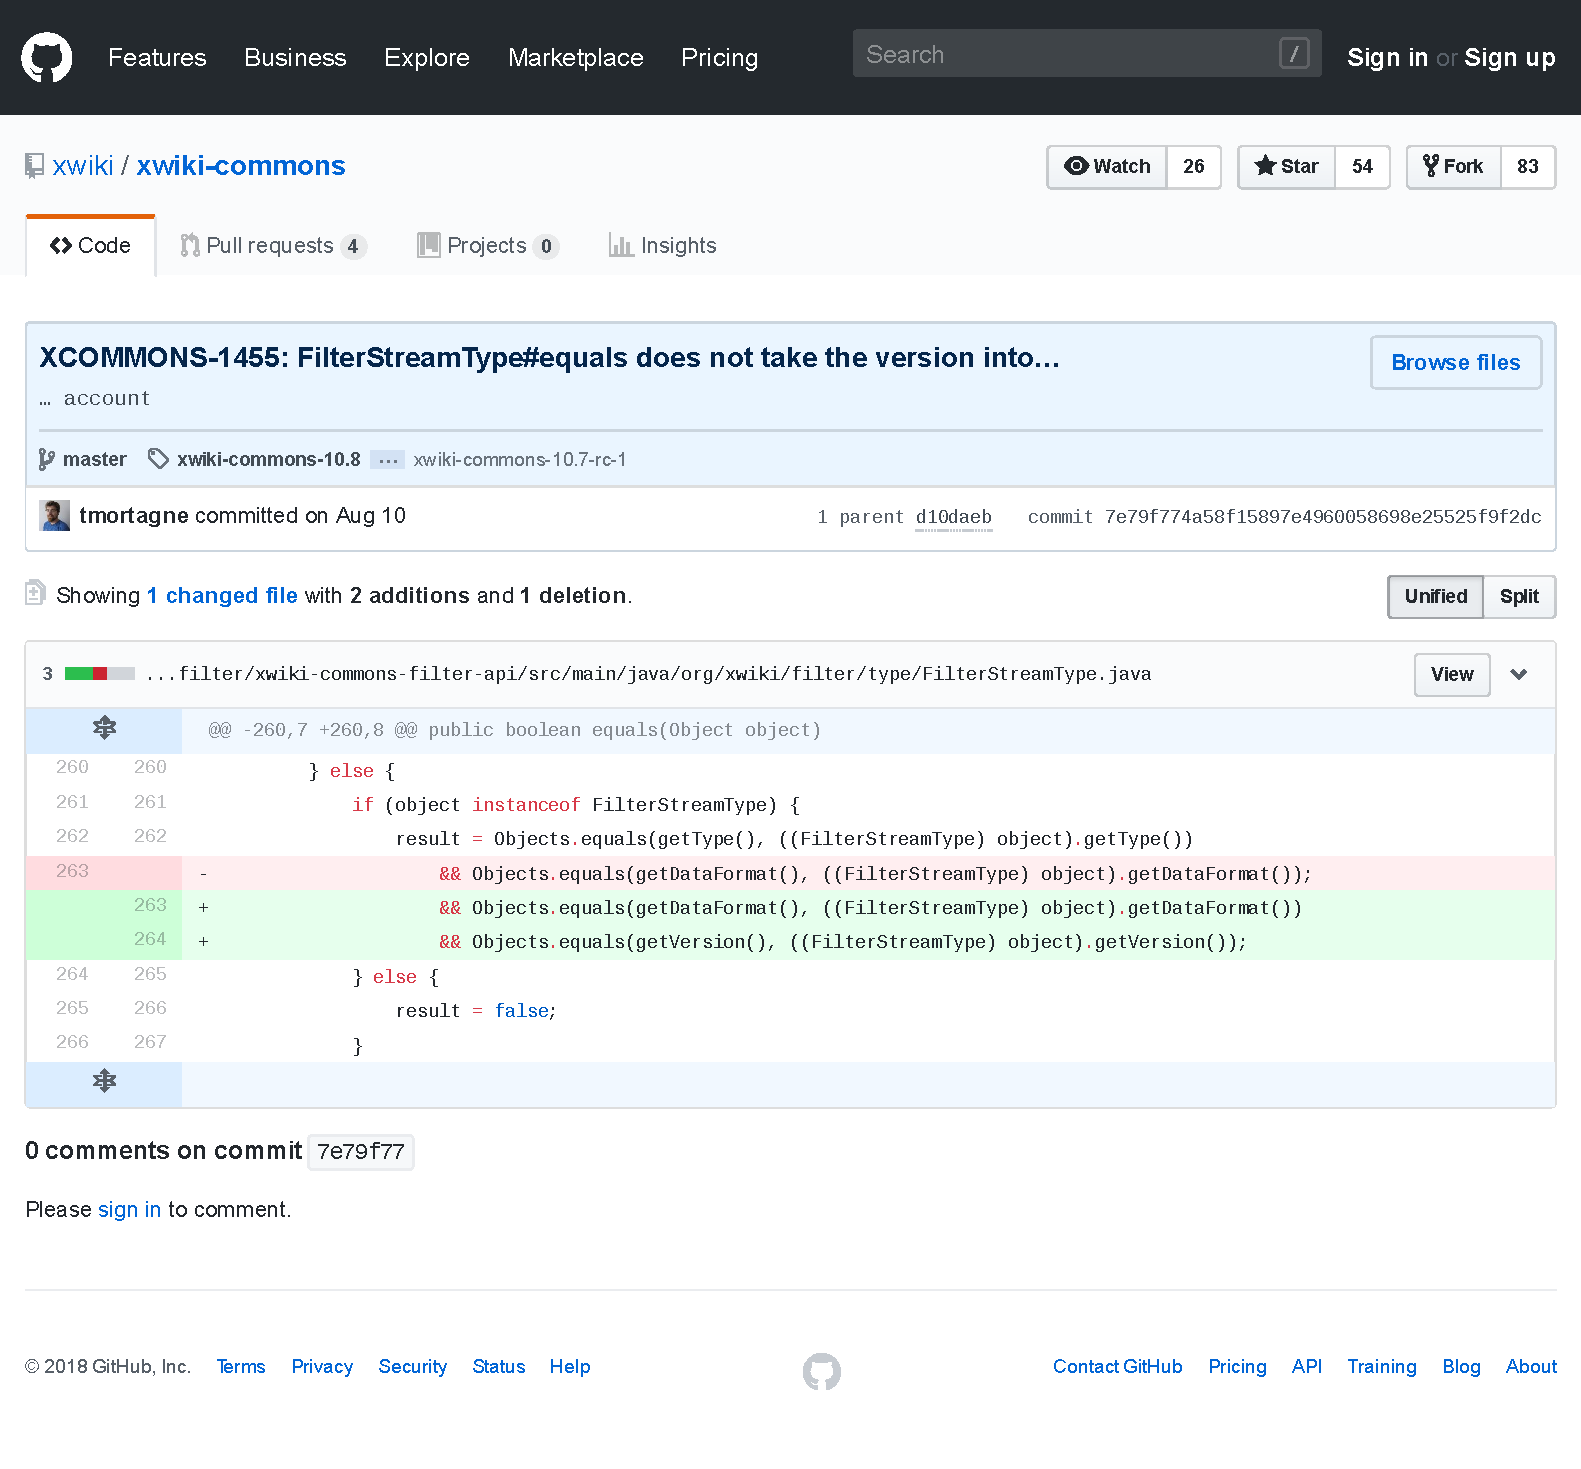
\includegraphics[width=.95\linewidth, trim=7.3cm 8.6cm 4.4cm 14.5cm, clip]{img/motivating_example.pdf}}
	\caption{Commit 7e79f77 on XWiki-Commons that changes the behavior without a test.}
	\label{fig:motivating_example}
\end{figure}

In this commit, the intent is to take into account the \texttt{version} (from method \texttt{getVersion}) in the \texttt{equals} method.
This change impacts the behavior of all methods that use it, \texttt{equals} being a highly used method.
Such a central behavioral change may impact the whole program, and the lack of a test case for this new behavior may have dramatic consequences in the future.
Without a test case, this change could be reverted and go undetected by the test suite and the Continuous Integration server, \ie the build would still pass.
Yet, a user of this program would encounter new errors, because of the changed behavior.
The developer took a risk when committing this change without a test case.

This extension of \dspot in continuous integration aims at mitigating such risk: 
test amplification aims at ensuring that every commit include a new test method or a modification of an existing test method.
In this chapter, I study \dspot's ability to automatically obtain a test method that highlights the behavioral change introduced by a commit.
This test method allows to identify the behavioral difference between the two versions of the program. 
The goal is to use this new test method to ensure that any changed behavior can be caught in the future.

What I propose is as follows: 
when Continuous Integration is triggered, 
rather than just executing the test suite to find regressions, 
it could also run an analysis of the commit to know if it contains a behavioral change, 
in the form of a new method or the modification of an existing one.
If there is no appropriate test method to detect a behavioral change, the approach would provide one. 
DCI would take as input the commit and a test suite, and generate a new test method that detects the behavioral change.

\subsection{Practibility}
\label{subsec:dci:background:praticability}

Following, a description of a complete scenario to sum up the vision of the approach's usage.

A developer commits a change into the program.
The Continuous Integration service is triggered;
the CI analyzes the commit.
There are two potential outcomes:
1) the developer provided a new test method or a modification to an existing one. 
In this case, the CI runs as usual, \eg it executes the test suite;
2) the developer did not provide a new test nor the modification of an existing one, the CI runs DCI on the commit to obtain a test method that detects the behavioral change and present it to the developer.
The developer can then validate the new test method that detects the behavioral change.
Following the test selection\autoref{subsec:dci:introduction:goal}, the new test method passes on the pre-commit version but fails on the post-commit version.
The current amplified test method cannot be added to the test suite, since it fails.
However, this test method is still useful, since one has only to negate the failing assertions, \eg change an \texttt{assertTrue} into an \texttt{assertFalse}, to obtain a valid and passing test method that explicitly executes the new behavior.
This can be done manually or automatically with approaches such as ReAssert\cite{ReAssert}.

\TODO{is this okay ? the definition of DSPOT says that dspot runs well on unit test}
From my experience, unit tests (vs integration test) are the best target for DCI
The reasons are behind the very nature of unit tests:
First, they have a small scope, which allow DCI to intensify its search while an integration test, that contains a lot of code, would make DCI explore the neighborhood in different ways.
Second, that is a consequence of the first, the unit tests are fast to be executed against integration test.
Since DCI needs to execute 5 times the tests under amplification, it means that DCI would be executed faster when it amplifies unit tests than when it amplified integration tests.

DCI has been designed to be easy to use.
The only cost of DCI is the time to set it up: in the ideal, happy-path case, it is meant to be a single command line through Maven goals.
Once DCI is set up in continuous integration, it automatically runs at each commit and developers directly benefit from amplified test methods that strengthen the existing test suite.

%
%   Behavioral Change
%
\subsection{Behavioral Change}
\label{subsec:dci:background:behavioral-change}

A \emph{behavioral change} is a source-code modification that triggers a new state for some inputs \cite{saff2004experimental}.
Considering the pre-commit version $P$ and the post-commit version $P'$ of a program, the commit introduces a behavioral change if it is possible to implement a test case that can trigger and observe the change, \ie, it passes on $P$ and fails on $P'$, or the opposite.
In short, the behavioral change must have an impact on the observable behavior of the program.

%
%   Behavioral Change Detection
%
\subsection{Behavioral Change Detection}
\label{subsec:dci:background:behavioral-change-detection}

Behavioral change detection is the task of identifying or generating a test or an input that distinguishes a behavioral change between two versions of the same program.
In this chapter, I propose a novel approach to detect behavioral changes based on test amplification.

% -----------------------
%  CONTRIBUTIONS
% -----------------------

\section{Behavioral Change Detection Approach}
\label{sec:dci:techniques}

\subsection{Overview of DCI}
\label{subsec:global_overview}

DCI takes as input a program, its test suite, and a commit modifying the program.
The commit, as done in version control systems, is basically the diff between two consecutive versions of the program.
%
% output
DCI outputs new test methods that detect the behavioral difference between the pre- and post-commit versions of the program.
The new tests pass on a given version, but fail on the other, demonstrating the presence of a behavioral change captured.% by an assertion.

DCI computes the code coverage of the diff and selects test methods accordingly. % to this diff coverage.
Then, it applies two kinds of test amplification to generate new test methods that detect the behavioral change.
%
\autoref{fig:global_approach} sums up the different phases of the approach:
1) Compute the diff coverage and select the tests to be amplified;
2) Amplify the selected tests based on the pre-commit version;
3) Execute amplified test methods against the post-commit version, and keep the failing test methods.
This process produces test methods that pass on the pre-commit version, fail on the post-commit version, hence they detect at least one behavioral change introduced by a given commit.

\begin{figure}
    \fbox{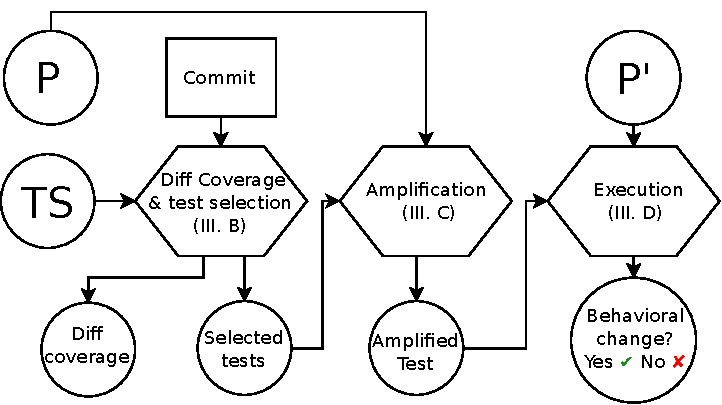
\includegraphics[width=.95\linewidth]{img/global_flow.pdf}}
    \caption{Overview of our approach to detect behavioral changes in commits.}
    \label{fig:global_approach}
\end{figure}

\subsection{Test Selection and Diff Coverage}
\label{subsec:compute_diff_coverage}
%We need to know which tests executed what lines of the diff.
DCI implements a feature that:
\begin{enumerate*}
\item reports the diff coverage of a commit, and
\item selects the set of unit tests that execute the diff.
\end{enumerate*}
%
To do so, DCI first computes the code coverage for the whole test suite.
Second, it identifies the test methods that hit the statements modified by the diff. 
Third, it produces the two outcomes elicited earlier: the diff coverage, computed as the ratio of statements in the diff covered by the test suite over the total number of statements in the diff and the list of test methods that cover the diff.
%
Then, we select only test methods that are present in pre-commit version (\ie, we ignore the test methods added in the commit, if any).
The final list of test methods that cover the diff is then used to seed the amplification process.

\subsection{Test Amplification}

Once we have the initial tests that cover the diff, we want to make them detect the behavioral change and assess the new behavior.
This process of extending the scope of a test case is called test amplification~\cite{zhang2012}.
In DCI, we build upon Xie's technique~\cite{TaoXie2006} and Tonella's evolutionary algorithm~\cite{tonella} to perform test amplification.

%   A-AMPL
\subsubsection{Assertion Amplification}
\label{subsec:aampl}

A test method consists of a setup and assertions.
The former is responsible for putting the program under test into a specific state; the latter is responsible for verifying that the actual state of the program at the end of the test is the expected one.
To do this, assertions compare actual values against expected values: if the assertion holds, the program is considered correct, if not, the test case has revealed the presence of a bug.

Assertion amplification (\aampl) has been proposed by \cite{TaoXie2006}.
It takes as input a program and its test suite, and it synthesizes new assertions on public methods that capture the program state.
The targeted public methods are those that take no parameter, return a result, and match a Java naming convention of getters, \eg the method starts with \emph{get} or \emph{is}. The standard method \emph{toString()} is also used.
If a method used returns a complex Java Object, \aampl recursively uses getters on this object to generate deeper assertions.

In case the test method sets the program into an incorrect state and an exception is thrown, \aampl generates a test for this exception by wrapping the test method body in a \emph{try/catch} block. 
It also inserts a \emph{fail} statement at the end of the body of the \emph{try}, \ie it means that if the exception is not thrown the test method fails.

\begin{algorithm}[h]
\begin{algorithmic}[1]
\Require{Program $P$}
\Require{Test Suite $TS$}
\Ensure{An Amplified Test Suite $ATS$}
\State{$ATS \leftarrow \emptyset$}
\For{$Test$ in $TS$}
    \State{$NoAssertTest \leftarrow removeAssertions(Test)$}
    \State{$InstrTest \leftarrow instrument(NoAssertTest)$}
    \State{$execute(InstrTest)$}
    \State{$AmplTest \leftarrow NoAssertTest.clone()$}
    \For{$Observ$ in $InstrTest.observations()$}
        \State{$Assert \leftarrow generateAssertion(Observ)$}
        \State{$AmplTest \leftarrow AmplTest.add(Assert)$}
    \EndFor
    \State{$ATS.add(select(AmplTest))$}
    \State{$ATS.add(AmplTest)$}
\EndFor
\Return $ATS$
\end{algorithmic}
\caption{\aampl: Assertion amplification algorithm.}
\label{algo:aampl}
\end{algorithm}

We present \aampl's pseudo-code in Algorithm \autoref{algo:aampl}. First, it initializes an empty set of tests $ATS$ (Line 1). 
For each $Test$ method in the test suite $TS$ (Line 2), it removes the existing assertions to obtain $NoAssertTest$ (Line 3). 
Then, it instruments $NoAssertTest$ with observation points (Line 4) that allow retrieving values from the program at runtime, which results in $InstrTest$. 
In order to collect the values, it executes $InstrTest$ (Line 5).
Eventually, for each observation $Observ$ of the set of observations from $InstrTest$ (Line 7 to 10), it generates an assertion (Line 8) and adds it to the amplified tests $AmplTest$ (Line 9).
At the end, it selects amplified test according to a specific test criterion using the method $select()$ (Line 11) and add selected amplified test methods to the set of test methods $AmplTest$, in other words, an amplified test suite (Line 13).

To sum up, \aampl increases the number of assertions. 
By construction, it specifies more behaviors than the original test suite.
DCI$_{AAMPL}$ is the \aampl mode for DCI.

%
%   I-AMPL
%
\subsubsection{Search-based Amplification}
\label{subsec:sbampl}
Search-based test amplification consists in running stochastic transformations on test code~\cite{tonella}.
%
For DCI$_{AAMPL}$, this process consists in
%of search-based amplification is as follows:
%\begin{enumerate}
a) generating a set of original test methods by applying code transformations;
b) running \aampl to synthesize new assertions for these amplified test methods;
%\item select amplified tests to be kept, according to a given test criterion;
c) repeating this process $nb$ times\footnote{by default, $nb=3$}, each time seeding with the previously amplified test methods.
%\end{enumerate}
%
This final step allows the search-based algorithm to explore more inputs, and thus improve the chance of triggering new behaviors.

\begin{algorithm}[h]
\begin{algorithmic}[1]
\Require{Program $P$}
\Require{Program $P'$}
\Require{Test Suite $TS$}
\Require{Iterations number $Nb$}
\Ensure{An Amplified Test Suite $ATS$}
\State{$ATS \leftarrow \emptyset$}
\State{$TmpTests \leftarrow \emptyset$}
\For{$Test$ in $TS$}
    \State{$TmpTests \leftarrow Test$}
    \For{$i \leftarrow 0, i < Nb$}
        \State{$TransformedTests \leftarrow transform(TmpTests)$}
        \State{$AmplifiedTests \leftarrow aampl(TransformedTests)$}
        %\STATE{$ATS.add(AmplifiedTests)$}
        \State{$ATS.add(select(AmplifiedTests))$}
        \State{$TmpTests \leftarrow AmplifiedTests$}
    \EndFor
\EndFor
\Return $ATS$
\end{algorithmic}
\caption{\sbampl: Search based amplification algorithm}
\label{algo:sbampl}
\end{algorithm}

We present the search-based amplification algorithm in Algorithm \autoref{algo:sbampl}.
This algorithm is a basic Hill Climbing algorithm.
It takes as input a program with two distinct versions $P$ and $P'$, its test suite $TS$ and a number of iterations $nb$, (in our case $nb=3$).
It produces an amplified test suite that contains test methods that pass on $P$ but fail on $P'$.
To do so, it initializes an empty set of amplified test methods $ATS$ (Line 1), which will be the final output, and $TmpTests$ (Line 2) which is a temporary set.
Then, for each test method in the test suite $TS$ (Line 3), it applies the following operations: 
1) transform the current set of test methods (Line 6) to obtain $TransformedTests$;
2) apply \aampl on $TransformedTests$ (Line 7, see \autoref{algo:aampl}) to obtain $AmplifiedTests$; 
3) select amplified test methods using the method $select()$, and add them to $ATS$ 
(the method $select()$ executes the amplified tests on $P'$ and keeps only tests that fail, \ie that detect a behavioral change);
and Finally, 4) affects $AmplifiedTests$ to $TmpTests$ in order to stack transformations.

In our study, we consider the following test transformations:
\begin{itemize}
\item On numbers:
    \begin{enumerate*}
        \item add 1 to an integer
        \item minus 1 to an integer
        \item replace an integer by zero
        \item replace an integer by the maximum value (Integer.MAX\_VALUE in Java)
        \item replace an integer by the minimum value (\texttt{Integer.MIN\_VALUE} in Java).
    \end{enumerate*}
\item On booleans:
    \begin{enumerate*}
        \item negate the value.
    \end{enumerate*}
\item On string literals:
    \begin{enumerate*}
        \item replace a string with another existing string 
        \item replace a string with white space, or a system path separator, or a system file separator.
        \item add 1 random character to the string
        \item remove 1 random character from the string
        \item replace 1 random character in the string by another random character
        \item replace the string with a random string of the same size
        \item replace the string with the \texttt{null} value
    \end{enumerate*}
\item On methods :
    \begin{enumerate*}
        \item remove a method call
        \item duplicate a method call
    \end{enumerate*}.
\end{itemize}

DCI$_{SBAMPL}$ is the search-based amplification mode for DCI.

\subsection{Execution and Change Detection}
\label{sec:change-detection}

The final step performed by DCI consists in checking whether that the amplified test methods detect behavioral changes.
Because DCI amplifies test methods using the pre-commit version, all amplified test methods pass on this version, by construction. 
Consequently, for the last step, DCI runs the amplified test methods only on the post-commit version. 
Every test that fails is in fact detecting a behavioral change introduced by the commit, and is a success. DCI keeps the tests that successfully detect behavioral changes.

\subsection{Implementation}
\label{sub:implementation}

DCI is implemented in Java and is built on top of the OpenClover and Gumtree~\cite{falleri:hal-01054552} libraries.
It computes the global coverage of the test suite with OpenClover, which instruments and executes the test suite.
Then, it uses Gumtree to have an AST representation of the diff.
DCI matches the diff with the test that executes those lines. 
Through its Maven plugin, DCI can be seamlessly implemented into continuous integration.
DCI is publicly available on \gh.\footnote{\url{https://github.com/STAMP-project/dspot.git}}

\section{Evaluation}
\label{sec:evaluation}

To evaluate the DCI approach, we design an experimental protocol to answer the following research questions:

\newcommand{\rqcharacteristics}{\RQ{1}{What are the characteristics of commits with behavioral changes in the context of continuous integration?}}
\newcommand{\rqdetection}{\RQ{1}{To what extent are DCI$_{AAMPL}$ and DCI$_{SBAMPL}$ able to produce amplified test methods that detect the behavioral changes?}}
\newcommand{\rqselection}{\RQ{3}{What is the effectiveness of our test selection method?}}
\newcommand{\rqhuman}{\RQ{4}{How do human and generated tests that detect behavioral changes differ?}}
\newcommand{\rqiteration}{\RQ{2}{What  is the impact of the number of iteration performed by  DCI$_{SBAMPL}$?}}

\noindent
\begin{itemize}
% \item \rqcharacteristics
\item \rqdetection
\item \rqiteration
\item \rqselection
\item \rqhuman
\end{itemize}

\subsection{Benchmark}
\label{sec:benchmark}
To the best of our knowledge, there is no benchmark of commits in Java with behavioral changes in the literature. Consequently, we devise a project and commit selection procedure in order to construct a benchmark for our approach.

\paragraph{Project selection}
We need software projects that are
1) publicly-available,
2) written in Java,
3) and use continuous integration.
%
We pick the projects from the dataset in \cite{descartes} and \cite{dspot-emse}, which is composed of mature Java projects from \gh.

\paragraph{Commit selection}
%To select commits, we apply the following procedure.
We take commits in inverse chronological order, from newest to oldest.
%this result in commits buildable and analyzable with the current version of build and test tools;
We select the first ten commits that match the following criteria:
1) the commit modifies Java files (most behavioral changes are source code changes.\footnote{We are aware that behavioral changes can be introduced in other ways, such as modifying dependencies or configuration files \cite{Test:Coverage:Evolution}.});
% ground-truth
2) the commit provides or modifies a manually written test that detects a behavioral change. 
To verify this property, we execute the test on the pre-commit version. 
If it fails, it means that the test detects at least 1 behavioral change.
We will use this test as a \textit{ground-truth test} in \textbf{RQ4}.
3) The changes of the commit must be covered by the pre-commit test suite.
To do so, we compute the diff coverage. 
If the coverage is 0\%, we discard the commit. 
We do this because if the change is not covered, we cannot select any test methods to be amplified, which is what we want to evaluate.

Together, these criteria ensure that all selected commits:
1) introduce behavioral changes,
2) provide or modify a manually written test case that detects a behavioral change (which will be used as ground-truth for comparing generated tests), and
3) that there is at least 1 test in the pre-commit version of the program that executes the diff and can be used to seed the amplification process.
4) There is no structural change in the commit between both versions, \eg no change in method signature and deletion of classes (this is ensured since the pre-commit test suite compiles and runs against the post-commit version of the program and vice-versa.)

\paragraph{Final benchmark}
\begin{table}[h]
\centering
\def\arraystretch{1}
\setlength\tabcolsep{0.8pt}
\caption{Considered Period for Selecting Commits.}
\begin{tabular}{lc|rr|cccc}
\hline
project &
LOC &
\begin{tabular}{c}start\\date\end{tabular}&
\begin{tabular}{c}end\\date\end{tabular}&
\begin{tabular}{c}\#total\\commits\end{tabular}&
\begin{tabular}{c}\#discarded\\commits\end{tabular}&
\begin{tabular}{c}\#matching\\commits\end{tabular}&
\begin{tabular}{c}\#selected\\commits\end{tabular}\\
\hline
\scriptsize{commons-io}	&	59607	&	9/10/2015	&	9/29/2018	&	385	&	375	&	16(4.16\%)	&	10	\\
\rowcolor[HTML]{EFEFEF}
\scriptsize{commons-lang}	&	77410	&	11/22/2017	&	10/9/2018	&	227	&	217	&	13(5.73\%)	&	10	\\
\scriptsize{gson}	&	49766	&	6/14/2016	&	10/9/2018	&	159	&	149	&	13(8.18\%)	&	10	\\
\rowcolor[HTML]{EFEFEF}
\scriptsize{jsoup}	&	20088	&	12/21/2017	&	10/10/2018	&	50	&	40	&	11(22.00\%)	&	10	\\
\scriptsize{mustache.java}	&	10289	&	7/6/2016	&	04/18/2019	&	68	&	58	&	11(16.18\%)	&	10	\\
\rowcolor[HTML]{EFEFEF}
\scriptsize{xwiki-commons}	&	87289	&	10/31/2017	&	9/29/2018	&	687	&	677	&	23(3.35\%)	&	10	\\
\end{tabular}
\label{tab:benchmark}
\end{table}

\autoref{tab:benchmark} shows the main statistics on the benchmark dataset. % construction.
The first column is the name of the considered project;
The second column is the date at which we did the analysis;
The third column is the date of the oldest commit for the project;
The fourth, fifth, sixth and seventh are respectively the total number of commit we analyze, the total number of commits we discard, the number of commits that match all our criteria but the third (there is no test in the pre-commit that execute the change and the number of commit we select).
We note that our benchmark is only composed of recent commits from notable open-source projects and is available on \gh at \url{https://github.com/STAMP-project/dspot-experiments}.

\subsection{Protocol}
\label{subsec:protocol}

%To answer \textbf{RQ1},
%we compute and study the main metrics of the commits in the benchmark. 
%we collect the following information for each commit:
%1) the date of the commit;
%2) the number of tests in the test suite at the date of the commit;
%3) the number of tests added or modified by the commit;
%4) the size of the diff, in terms of line insertions and deletions;
%5) the coverage of the diff by the test suite.

To answer \textbf{RQ1}, we run DCI$_{AAMPL}$ and DCI$_{SBAMPL}$ on the benchmark projects.
We then report the total number of behavioral changes successfully detected by DCI, \ie the number of commits for which DCI generates at least 1 test method that passes on the pre-commit version but fails on the post-commit version.
We also discuss 1 case study of a successful behavioral change detection.

To answer \textbf{RQ2}, we run DCI$_{SBAMPL}$ for 1, 2 and 3 iterations on the benchmark projects.
We report the number of behavioral changes successfully detected for each number of iterations in the main loop.
We report also the number amplified test methods that detect the behavioral changes for each commit for 10 different seeds to study the impact of the randomness on the output of DSpot
We perform a Kruskal-Wallis test statistic on these numbers.

The null hypothesis is the following: The population median of all of the groups are equal

The alternative hypothesis is: at least one population median of one group is different from the population median of at least one other group

We take a confidence level of 95\%, or $\alpha = 0.05$.

For \textbf{RQ3}, the test selection method is considered effective if the tests selected to be amplified semantically relate to the code changed by the commit. 
To assess this, we perform a manual analysis.% as follows.
We randomly select 1 commit per project in the benchmark, and we manually analyze whether the automatically selected tests for this commit are semantically related to the behavioral changes in the commit. 
%This research question aims at validating the test selection according to a diff of DCI.

To answer \textbf{RQ4}, we use the ground-truth tests written or modified by developers in the selected commits. % written by the humans.
We manually compare the amplified test methods that detect behavioral changes to the human tests, for 1 commit per project.
%For this, we take only consider commits for which DCI has been able to produce at least one test method that detects the behavioral change. 

\subsection{Results}
\label{subsec:result}
\begin{table}
\centering
\small
\def\arraystretch{0.3}%  1 is the default, change whatever you need
\setlength\tabcolsep{.35pt} % default value: 6pt
\caption{Performance evaluation of DCI on 60 commits from 6 large open-source projects.}
%\rotvertical{
\label{tab:overall_result}
\begin{tabular}{l|c|rcccc|c|cc|cc|cc|cc}
&
id&
date&
\#Test&
\begin{tabular}{c}\#Modified\\Tests\end{tabular}&
{\color{ForestGreen}{+\xspace}} / {\color{red}{-\xspace}}&
Cov&
\begin{tabular}{c}\#Selected\\Tests\end{tabular}&
\begin{tabular}{c}\#\aampl\\Tests\end{tabular}&
Time&
\begin{tabular}{c}\#\sbampl\\Tests\end{tabular}&
Time\\\\
\hline
\multirow{11}{*}{\rotvertical{commons-io}}
&  c6b8a38  &  6/12/18 &  1348  &  2  &  {\color{ForestGreen}{104\xspace}} / {\color{red}{3\xspace}}  &  100.0  &  3  &  0  &  10.0s  &  0  &  98.0s\\
&  2736b6f  &  12/21/17 &  1343  &  2  &  {\color{ForestGreen}{164\xspace}} / {\color{red}{1\xspace}}  &  1.79  &  8  &  0  &  19.0s  &  \cmark(12)  &  76.3m\\
&  a4705cc  &  4/29/18 &  1328  &  1  &  {\color{ForestGreen}{37\xspace}} / {\color{red}{0\xspace}}  &  100.0  &  2  &  0  &  10.0s  &  0  &  38.1m\\
&  f00d97a  &  5/2/17 &  1316  &  10  &  {\color{ForestGreen}{244\xspace}} / {\color{red}{25\xspace}}  &  100.0  &  2  &  \cmark(1)  &  10.0s  &  \cmark(39)  &  27.0s\\
&  3378280  &  4/25/17 &  1309  &  2  &  {\color{ForestGreen}{5\xspace}} / {\color{red}{5\xspace}}  &  100.0  &  1  &  \cmark(1)  &  9.0s  &  \cmark(11)  &  24.0s\\
&  703228a  &  12/2/16 &  1309  &  1  &  {\color{ForestGreen}{6\xspace}} / {\color{red}{0\xspace}}  &  50.0  &  8  &  0  &  19.0s  &  0  &  71.0m\\
&  a7bd568  &  9/24/16 &  1163  &  1  &  {\color{ForestGreen}{91\xspace}} / {\color{red}{83\xspace}}  &  50.0  &  8  &  0  &  20.0s  &  0  &  65.2m\\
&  81210eb  &  6/2/16 &  1160  &  1  &  {\color{ForestGreen}{10\xspace}} / {\color{red}{2\xspace}}  &  100.0  &  1  &  0  &  8.0s  &  \cmark(8)  &  23.0s\\
&  57f493a  &  11/19/15 &  1153  &  1  &  {\color{ForestGreen}{15\xspace}} / {\color{red}{1\xspace}}  &  100.0  &  8  &  0  &  7.0s  &  0  &  54.0s\\
&  5d072ef  &  9/10/15 &  1125  &  12  &  {\color{ForestGreen}{74\xspace}} / {\color{red}{34\xspace}}  &  68.42  &  25  &  \cmark(6)  &  29.0s  &  \cmark(1538)  &  2.2h\\
\hline
\rowcolor[HTML]{EFEFEF}
&  total  &  \xspace{} &  \xspace{}  &  \xspace{}  &  \xspace{}  &  \xspace{}  &  66  &  0.80  &  avg(14.5s)  &  160.80  &  avg(38.8m)\\
\hline
\multirow{11}{*}{\rotvertical{commons-lang}}
&  f56931c  &  7/2/18 &  4105  &  1  &  {\color{ForestGreen}{30\xspace}} / {\color{red}{4\xspace}}  &  25.0  &  42  &  0  &  2.4m  &  0  &  8.6h\\
&  87937b2  &  5/22/18 &  4101  &  1  &  {\color{ForestGreen}{114\xspace}} / {\color{red}{0\xspace}}  &  77.78  &  16  &  0  &  35.0s  &  0  &  18.1m\\
&  09ef69c  &  5/18/18 &  4100  &  1  &  {\color{ForestGreen}{10\xspace}} / {\color{red}{1\xspace}}  &  100.0  &  4  &  0  &  16.0s  &  0  &  98.8m\\
&  3fadfdd  &  5/10/18 &  4089  &  1  &  {\color{ForestGreen}{7\xspace}} / {\color{red}{1\xspace}}  &  100.0  &  9  &  0  &  17.0s  &  \cmark(4)  &  17.2m\\
&  e7d16c2  &  5/9/18 &  4088  &  1  &  {\color{ForestGreen}{13\xspace}} / {\color{red}{1\xspace}}  &  33.33  &  7  &  0  &  16.0s  &  \cmark(2)  &  15.1m\\
&  50ce8c4  &  3/8/18 &  4084  &  4  &  {\color{ForestGreen}{40\xspace}} / {\color{red}{1\xspace}}  &  90.91  &  2  &  \cmark(1)  &  28.0s  &  \cmark(135)  &  2.0m\\
&  2e9f3a8  &  2/11/18 &  4084  &  2  &  {\color{ForestGreen}{79\xspace}} / {\color{red}{4\xspace}}  &  30.0  &  47  &  0  &  79.0s  &  0  &  66.5m\\
&  c8e61af  &  2/10/18 &  4082  &  1  &  {\color{ForestGreen}{8\xspace}} / {\color{red}{1\xspace}}  &  100.0  &  10  &  0  &  17.0s  &  0  &  16.0s\\
&  d8ec011  &  11/12/17 &  4074  &  1  &  {\color{ForestGreen}{11\xspace}} / {\color{red}{1\xspace}}  &  100.0  &  5  &  0  &  31.0s  &  0  &  2.3m\\
&  7d061e3  &  11/22/17 &  4073  &  1  &  {\color{ForestGreen}{16\xspace}} / {\color{red}{1\xspace}}  &  100.0  &  8  &  0  &  17.0s  &  0  &  11.4m\\
\hline
\rowcolor[HTML]{EFEFEF}
&  total  &  \xspace{} &  \xspace{}  &  \xspace{}  &  \xspace{}  &  \xspace{}  &  150  &  0.10  &  avg(40.5s)  &  14.10  &  avg(74.7m)\\
\hline
\multirow{11}{*}{\rotvertical{gson}}
&  b1fb9ca  &  9/22/17 &  1035  &  1  &  {\color{ForestGreen}{23\xspace}} / {\color{red}{0\xspace}}  &  50.0  &  166  &  0  &  4.2m  &  0  &  92.5m\\
&  7a9fd59  &  9/18/17 &  1033  &  2  &  {\color{ForestGreen}{21\xspace}} / {\color{red}{2\xspace}}  &  83.33  &  14  &  0  &  15.0s  &  \cmark(108)  &  2.1m\\
&  03a72e7  &  8/1/17 &  1031  &  2  &  {\color{ForestGreen}{43\xspace}} / {\color{red}{11\xspace}}  &  68.75  &  371  &  0  &  7.7m  &  0  &  3.2h\\
&  74e3711  &  6/20/17 &  1029  &  1  &  {\color{ForestGreen}{68\xspace}} / {\color{red}{5\xspace}}  &  8.0  &  1  &  0  &  4.0s  &  0  &  16.0s\\
&  ada597e  &  5/31/17 &  1029  &  2  &  {\color{ForestGreen}{28\xspace}} / {\color{red}{3\xspace}}  &  100.0  &  5  &  0  &  8.0s  &  0  &  8.7m\\
&  a300148  &  5/31/17 &  1027  &  7  &  {\color{ForestGreen}{103\xspace}} / {\color{red}{2\xspace}}  &  18.18  &  665  &  0  &  9.2m  &  \cmark(6)  &  4.9h\\
&  9a24219  &  4/19/17 &  1019  &  1  &  {\color{ForestGreen}{13\xspace}} / {\color{red}{1\xspace}}  &  100.0  &  36  &  0  &  2.2m  &  0  &  48.9m\\
&  9e6f2ba  &  2/16/17 &  1018  &  2  &  {\color{ForestGreen}{56\xspace}} / {\color{red}{2\xspace}}  &  50.0  &  9  &  0  &  32.0s  &  \cmark(2)  &  8.5m\\
&  44cad04  &  11/26/16 &  1015  &  1  &  {\color{ForestGreen}{6\xspace}} / {\color{red}{0\xspace}}  &  100.0  &  2  &  0  &  15.0s  &  \cmark(37)  &  40.0s\\
&  b2c00a3  &  6/14/16 &  1012  &  4  &  {\color{ForestGreen}{242\xspace}} / {\color{red}{29\xspace}}  &  60.71  &  383  &  0  &  7.9m  &  0  &  3.6h\\
\hline
\rowcolor[HTML]{EFEFEF}
&  total  &  \xspace{} &  \xspace{}  &  \xspace{}  &  \xspace{}  &  \xspace{}  &  1652  &  0.00  &  avg(3.2m)  &  15.30  &  avg(86.5m)\\
\hline
\multirow{11}{*}{\rotvertical{jsoup}}
&  426ffe7  &  5/11/18 &  668  &  4  &  {\color{ForestGreen}{27\xspace}} / {\color{red}{46\xspace}}  &  64.71  &  27  &  \cmark(2)  &  42.0s  &  \cmark(198)  &  33.6m\\
&  a810d2e  &  4/29/18 &  666  &  1  &  {\color{ForestGreen}{27\xspace}} / {\color{red}{1\xspace}}  &  80.0  &  5  &  0  &  10.0s  &  0  &  26.6m\\
&  6be19a6  &  4/29/18 &  664  &  1  &  {\color{ForestGreen}{23\xspace}} / {\color{red}{1\xspace}}  &  50.0  &  50  &  0  &  69.0s  &  0  &  67.7m\\
&  e38dfd4  &  4/28/18 &  659  &  1  &  {\color{ForestGreen}{66\xspace}} / {\color{red}{15\xspace}}  &  90.0  &  18  &  0  &  35.0s  &  0  &  12.5m\\
&  e9feec9  &  4/15/18 &  654  &  1  &  {\color{ForestGreen}{15\xspace}} / {\color{red}{3\xspace}}  &  100.0  &  4  &  0  &  9.0s  &  0  &  95.0s\\
&  0f7e0cc  &  4/14/18 &  653  &  2  &  {\color{ForestGreen}{56\xspace}} / {\color{red}{15\xspace}}  &  84.62  &  330  &  0  &  6.5m  &  \cmark(36)  &  11.8h\\
&  2c4e79b  &  4/14/18 &  650  &  2  &  {\color{ForestGreen}{82\xspace}} / {\color{red}{2\xspace}}  &  50.0  &  44  &  0  &  67.0s  &  0  &  4.7h\\
&  e5210d1  &  12/22/17 &  647  &  1  &  {\color{ForestGreen}{3\xspace}} / {\color{red}{3\xspace}}  &  100.0  &  14  &  0  &  9.0s  &  0  &  4.9m\\
&  df272b7  &  12/22/17 &  647  &  2  &  {\color{ForestGreen}{17\xspace}} / {\color{red}{1\xspace}}  &  100.0  &  13  &  0  &  9.0s  &  0  &  4.6m\\
&  3676b13  &  12/21/17 &  648  &  6  &  {\color{ForestGreen}{104\xspace}} / {\color{red}{12\xspace}}  &  38.46  &  239  &  0  &  6.2m  &  \cmark(52)  &  6.8h\\
\hline
\rowcolor[HTML]{EFEFEF}
&  total  &  \xspace{} &  \xspace{}  &  \xspace{}  &  \xspace{}  &  \xspace{}  &  744  &  0.20  &  avg(101.0s)  &  28.60  &  avg(2.6h)\\
\hline
\multirow{11}{*}{\rotvertical{mustache.java}}
&  a1197f7  &  1/25/18 &  228  &  1  &  {\color{ForestGreen}{43\xspace}} / {\color{red}{57\xspace}}  &  77.78  &  131  &  0  &  11.8m  &  \cmark(204)  &  10.1h\\
&  8877027  &  11/19/17 &  227  &  1  &  {\color{ForestGreen}{22\xspace}} / {\color{red}{2\xspace}}  &  33.33  &  47  &  0  &  7.3m  &  0  &  100.2m\\
&  d8936b4  &  2/1/17 &  219  &  2  &  {\color{ForestGreen}{46\xspace}} / {\color{red}{6\xspace}}  &  60.0  &  168  &  0  &  12.7m  &  0  &  84.2m\\
&  88718bc  &  1/25/17 &  216  &  2  &  {\color{ForestGreen}{29\xspace}} / {\color{red}{1\xspace}}  &  100.0  &  1  &  \cmark(1)  &  7.0s  &  \cmark(149)  &  3.7m\\
&  339161f  &  9/23/16 &  214  &  2  &  {\color{ForestGreen}{32\xspace}} / {\color{red}{10\xspace}}  &  77.78  &  123  &  0  &  8.6m  &  \cmark(1312)  &  5.8h\\
&  774ae7a  &  8/10/16 &  214  &  2  &  {\color{ForestGreen}{17\xspace}} / {\color{red}{2\xspace}}  &  100.0  &  11  &  0  &  66.0s  &  \cmark(124)  &  6.8m\\
&  94847cc  &  7/29/16 &  214  &  2  &  {\color{ForestGreen}{17\xspace}} / {\color{red}{2\xspace}}  &  100.0  &  95  &  0  &  11.5m  &  \cmark(2509)  &  21.4h\\
&  eca08ca  &  7/14/16 &  212  &  4  &  {\color{ForestGreen}{47\xspace}} / {\color{red}{10\xspace}}  &  80.0  &  18  &  0  &  87.0s  &  0  &  41.8m\\
&  6d7225c  &  7/7/16 &  212  &  2  &  {\color{ForestGreen}{42\xspace}} / {\color{red}{4\xspace}}  &  80.0  &  18  &  0  &  87.0s  &  0  &  40.1m\\
&  8ac71b7  &  7/6/16 &  210  &  10  &  {\color{ForestGreen}{167\xspace}} / {\color{red}{31\xspace}}  &  40.0  &  20  &  0  &  2.1m  &  \cmark(124)  &  5.6m\\
\hline
\rowcolor[HTML]{EFEFEF}
&  total  &  \xspace{} &  \xspace{}  &  \xspace{}  &  \xspace{}  &  \xspace{}  &  632  &  0.10  &  avg(5.8m)  &  442.20  &  avg(4.2h)\\
\hline
\multirow{11}{*}{\rotvertical{xwiki-commons}}
&  ffc3997  &  7/27/18 &  1081  &  0  &  {\color{ForestGreen}{125\xspace}} / {\color{red}{18\xspace}}  &  21.05  &  1  &  0  &  29.0s  &  0  &  18.0s\\
&  ced2635  &  8/13/18 &  1081  &  1  &  {\color{ForestGreen}{21\xspace}} / {\color{red}{14\xspace}}  &  60.0  &  5  &  0  &  93.0s  &  0  &  2.5h\\
&  10841b1  &  8/1/18 &  1061  &  1  &  {\color{ForestGreen}{107\xspace}} / {\color{red}{19\xspace}}  &  30.0  &  51  &  0  &  5.7m  &  0  &  3.4h\\
&  848c984  &  7/6/18 &  1074  &  1  &  {\color{ForestGreen}{154\xspace}} / {\color{red}{111\xspace}}  &  17.65  &  1  &  0  &  28.0s  &  0  &  18.0s\\
&  adfefec  &  6/27/18 &  1073  &  1  &  {\color{ForestGreen}{17\xspace}} / {\color{red}{14\xspace}}  &  40.0  &  22  &  \cmark(1)  &  76.0s  &  \cmark(3)  &  14.9m\\
&  d3101ae  &  1/18/18 &  1062  &  2  &  {\color{ForestGreen}{71\xspace}} / {\color{red}{9\xspace}}  &  20.0  &  4  &  \cmark(1)  &  72.0s  &  \cmark(31)  &  41.4m\\
&  a0e8b77  &  1/18/18 &  1062  &  2  &  {\color{ForestGreen}{51\xspace}} / {\color{red}{8\xspace}}  &  42.86  &  4  &  \cmark(1)  &  72.0s  &  \cmark(60)  &  42.1m\\
&  78ff099  &  12/19/17 &  1061  &  1  &  {\color{ForestGreen}{16\xspace}} / {\color{red}{0\xspace}}  &  33.33  &  2  &  0  &  68.0s  &  \cmark(4)  &  6.6m\\
&  1b79714  &  11/13/17 &  1060  &  1  &  {\color{ForestGreen}{20\xspace}} / {\color{red}{5\xspace}}  &  60.0  &  22  &  0  &  78.0s  &  0  &  17.9m\\
&  6dc9059  &  10/31/17 &  1060  &  1  &  {\color{ForestGreen}{4\xspace}} / {\color{red}{14\xspace}}  &  88.89  &  22  &  0  &  79.0s  &  0  &  20.5m\\
\hline
\rowcolor[HTML]{EFEFEF}
&  total  &  \xspace{} &  \xspace{}  &  \xspace{}  &  \xspace{}  &  \xspace{}  &  134  &  0.30  &  avg(94.3s)  &  9.80  &  avg(49.5m)\\
\hline
\hline
&  total  &  \xspace{} &  \xspace{}  &  \xspace{}  &  \xspace{}  &  \xspace{}  &  3378  &  9(15)  &  avg(2.2m)  &  28(6708)  &  avg(109.4m)\\
\hline
\end{tabular}
%}
\end{table}

The overall results are reported in \autoref{tab:overall_result}.
The first column is the shortened commit id;
the second column is the commit date;
the third column column is the total number of test methods executed when building that version of the project;
the fourth and fifth columns are respectively the number of tests modified or added by the commit, and the size of the diff in terms of line additions (in green) and deletions (in red);
the sixth and seventh columns are respectively the diff coverage and the number of tests DCI selected;
the eighth column provides the amplification results for DCI$_{AAMPL}$, and it is either a \cmark with the number of amplified tests that detect a behavioral change or a \textit{-} if DCI did not succeed in generating a test that detects a change;
the ninth column displays the time spent on the amplification phase;
The tenth and the eleventh are respectively a \cmark with the number of amplified tests for DCI$_{SBAMPL}$  (or - if a change is not detected) for 3 iterations.

\subsubsection{Characteristics of commits with behavioral changes in the context of continuous integration}
\label{subsubsec:answerq1}

%We consider the first columns (under \textbf{RQ1} meta column) of \autoref{tab:overall_result}, which describe the characteristics of our novel benchmark.
%The columns under the \textbf{RQ1} meta column
In  this section, we describe the the characteristics of commits introducing behavioral changes in the context of continuous integration
The first five columns in \autoref{tab:overall_result} describe the characteristics of our benchmark.
% date
The commit dates show that the benchmark is only composed of recent commits.
The most recent is \textsc{gson\#b1fb9ca}, authored 9/22/18, and the oldest is \textsc{commons-io\#5d072ef}, authored 9/10/15.
% now the number of tests
The number of test methods at the time of the commit shows two aspects of our benchmark:
1) we only have strongly tested projects;
2) we see that the number of tests evolve over time
%, witnessing the presence of 
due to test evolution.
%The fourth column shows that 
Every commit in the benchmark comes with test modifications (new tests or updated tests), and commit sizes are quite diverse.
%For instance, the first commit c6b8a38 has two modified tests.
%The fifth column shows the size of the commit diff in terms of added and removed lines.
%Overall, our selection criteria include a diversity of commit sizes. 
The three smallest commits are \textsc{commons-io\#703228a}, \textsc{gson\#44cad04} and \textsc{jsoup\#e5210d1} with 6 modifications, and the largest is \textsc{Gson\#45511fd} with 334 modifications.
%
Finally, 
%we consider the sixth column which gives the code coverage of the diff itself. 
on average, commits have 66.11\% coverage. 
The distribution of diff coverage is reported graphically by \autoref{fig:histdiffcoverage}: 
in commons-io all selected commits have more than 75\% coverage.
In XWiki-Commons, only 50\% of commits have more than 75\% coverage. Overall, 31 / 60 commits have at least 75\% of the changed lines covered.
This validates the correct implementation of our selection criteria that ensures the presence of a test specifying the behavioral change.

\begin{figure}
\centering
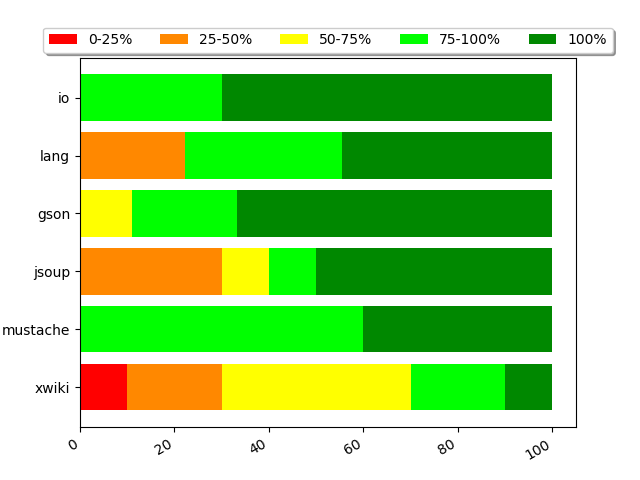
\includegraphics[width=.95\linewidth]{img/diff_cov_hist.png}
\caption{Distribution of diff coverage per project of our benchmark.}
\label{fig:histdiffcoverage}
\end{figure}

% recap of RQ1.
Thanks to our selection criteria, we have a curated benchmark of 50 commits with a behavioral change, coming from notable open-source projects, and covering a diversity of commit sizes. The benchmark is publicly available and documented for future research on this topic.

%%%%%%%%%%%%%%%%%%%%%%%%%%%%%%%%%%%%%%%%%%%%%%%%%%%%%
%%%%%%%%%%%%%%%%%%%%%%%%%%%%%%%%%%%%%%%%%%%%%%%%%%%%%
%% RESULTS RQ2
%%%%%%%%%%%%%%%%%%%%%%%%%%%%%%%%%%%%%%%%%%%%%%%%%%%%%
%%%%%%%%%%%%%%%%%%%%%%%%%%%%%%%%%%%%%%%%%%%%%%%%%%%%%
\subsubsection{\rqdetection}
\label{subsubsec:answerq2}

We now focus on the last 4 columns of \autoref{tab:overall_result}.
For instance, for \textsc{commons-io\#f00d97a} (4$^{th}$ row), DCI$_{AAMPL}$ generated 39 amplified tests that detect the behavioral change. 
For \textsc{commons-io\#81210eb} (8$^{th}$ row), only the \sbampl version of DCI detects the change.
%
Overall, using only \aampl, DCI generates amplified tests that detect 9 out of 60 behavioral changes.
Meanwhile, using \sbampl only, DCI generates amplified tests that detect 28 out of 60 behavioral changes.

Regarding the number of generated tests.
\DCII generates a large number of test cases, compared to \DCIA only (15 versus 6708, see column ``total'' at the bottom of the table). 
Both \DCIA and \DCIA can generate amplified tests, however since \DCIA does not produce a large amount of test methods the developers do not have to triage a large set of test cases. 
Also, since \DCIA only adds assertions, the amplified tests are easier to understand than the ones generated by \DCII.

% time
\DCII takes more time than \DCIA (for successful cases 38.7 seconds versus 3.3 hours on average).
The difference comes from the time consumed during the exploration of the input space in the case of \DCII, while \DCIA focuses on the amplification of assertions only, which represents a much smaller space of solutions. 

Overall, DCI successfully generates amplified tests that detect a behavioral change in 46\% of the commits in our benchmark(28 out of 60).
Recall that the 60 commits that we analyze are real changes that fix bugs in complex code bases.
They represent modifications, sometimes deep in the code, that represent challenges with respect to testability~\cite{voas1995software}.
Consequently, the fact DCI can generate test cases that detect behavioral changes, is considered an achievement.
The commits for which DCI fails to detect the change can be considered as a target for future research on this topic.

Now, we manually analyze a successful case where DCI detects the behavioral change.
We select commit \textsc{3fadfdd}\footnote{\url{https://github.com/apache/commons-lang/commit/3fadfdd}} from commons-lang, which is succinct enough to be discussed in the paper.
The diff is shown in \autoref{fig:diff_commons_lang_success}.

\begin{figure}[h]
\centering
\fbox{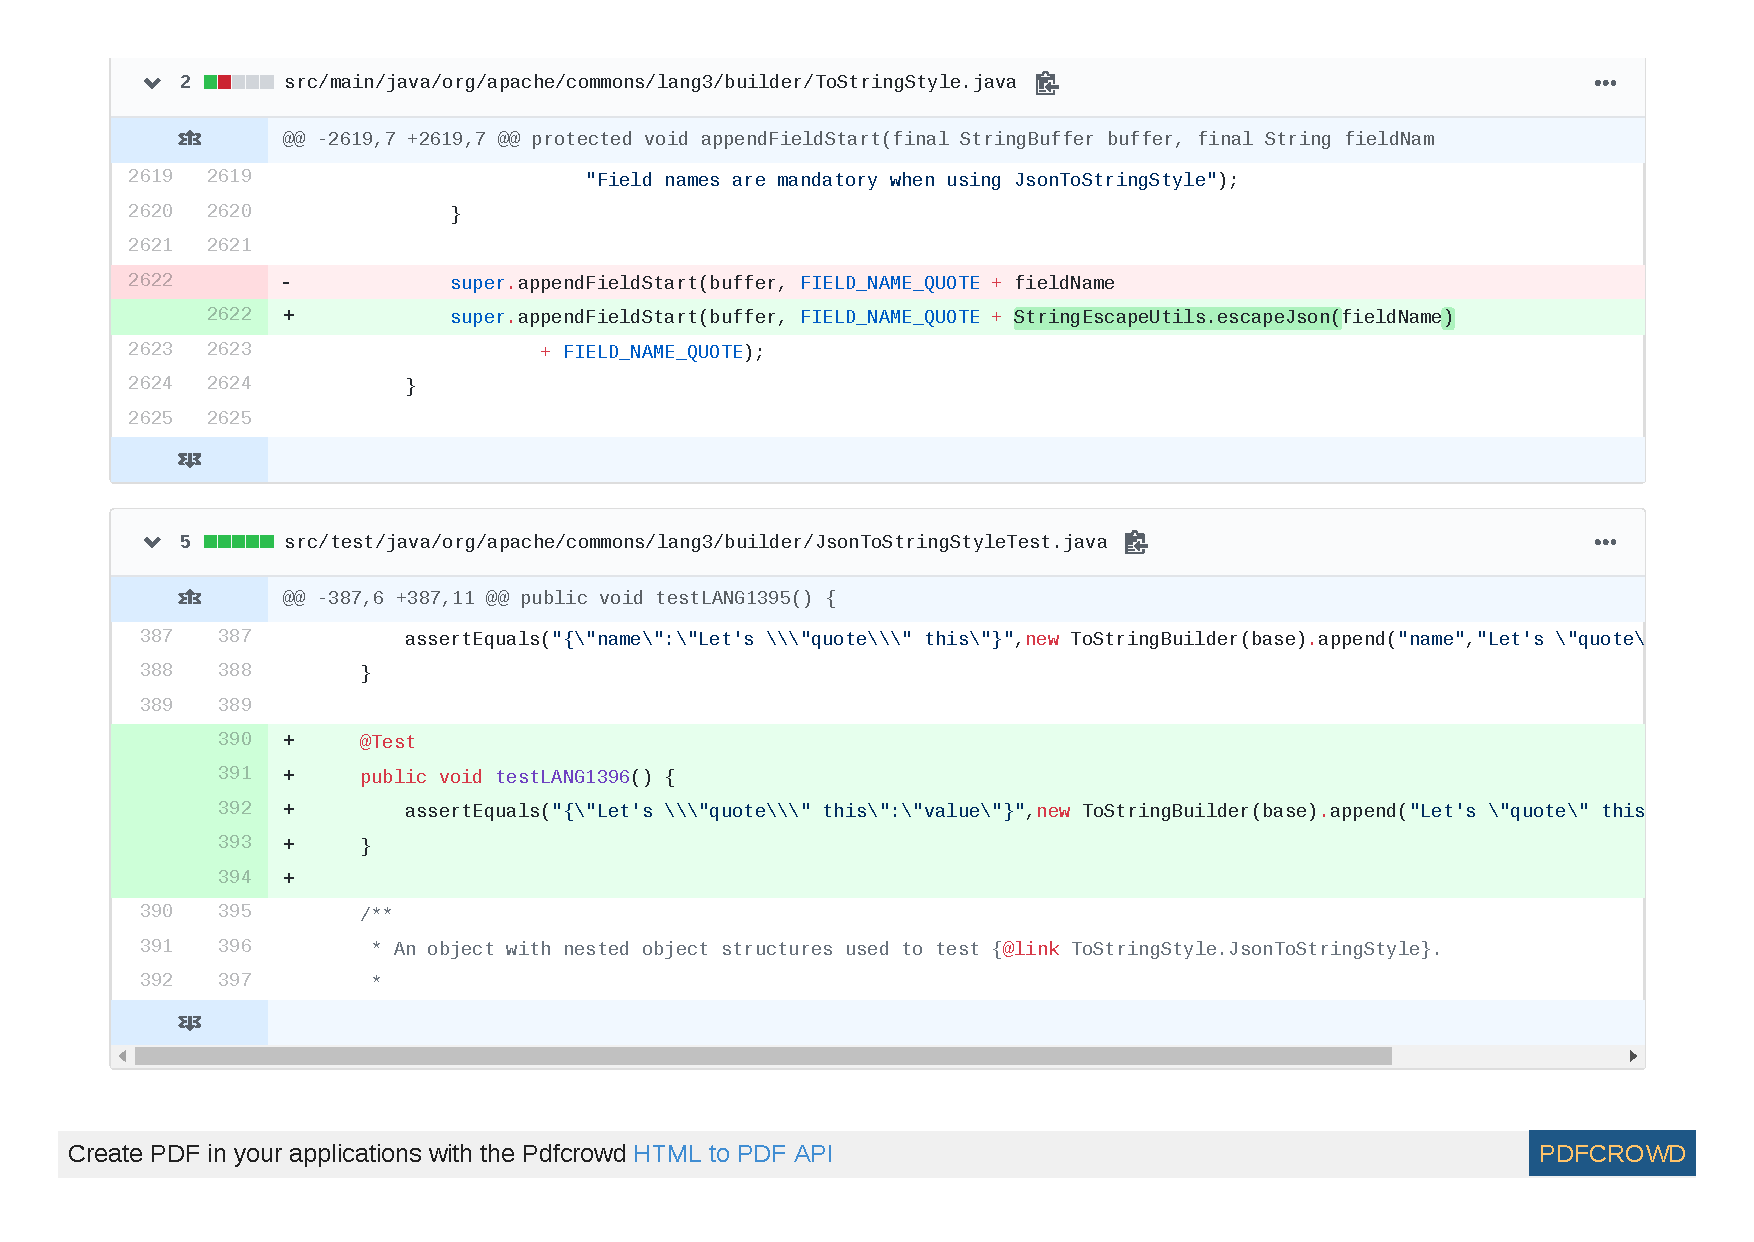
\includegraphics[width=.95\linewidth, trim=4.5cm 14.85cm 6.5cm 4.3cm, clip]{img/diff/success-diff-commons-lang.pdf}}
\caption{Diff of commit \textsc{3fadfdd} from commons-lang.}
\label{fig:diff_commons_lang_success}
\end{figure}

The developer added a method call to a method that escapes specials characters in a string. 
The changes come with a new test method that specifies the new behavior. 

DCI starts the amplification from the \texttt{testNestingPerson} test method defined in \texttt{JsonToStringStyleTest}. The test is selected for amplification because it triggers the execution of the changed line.

\begin{figure}[h]
\centering
\fbox{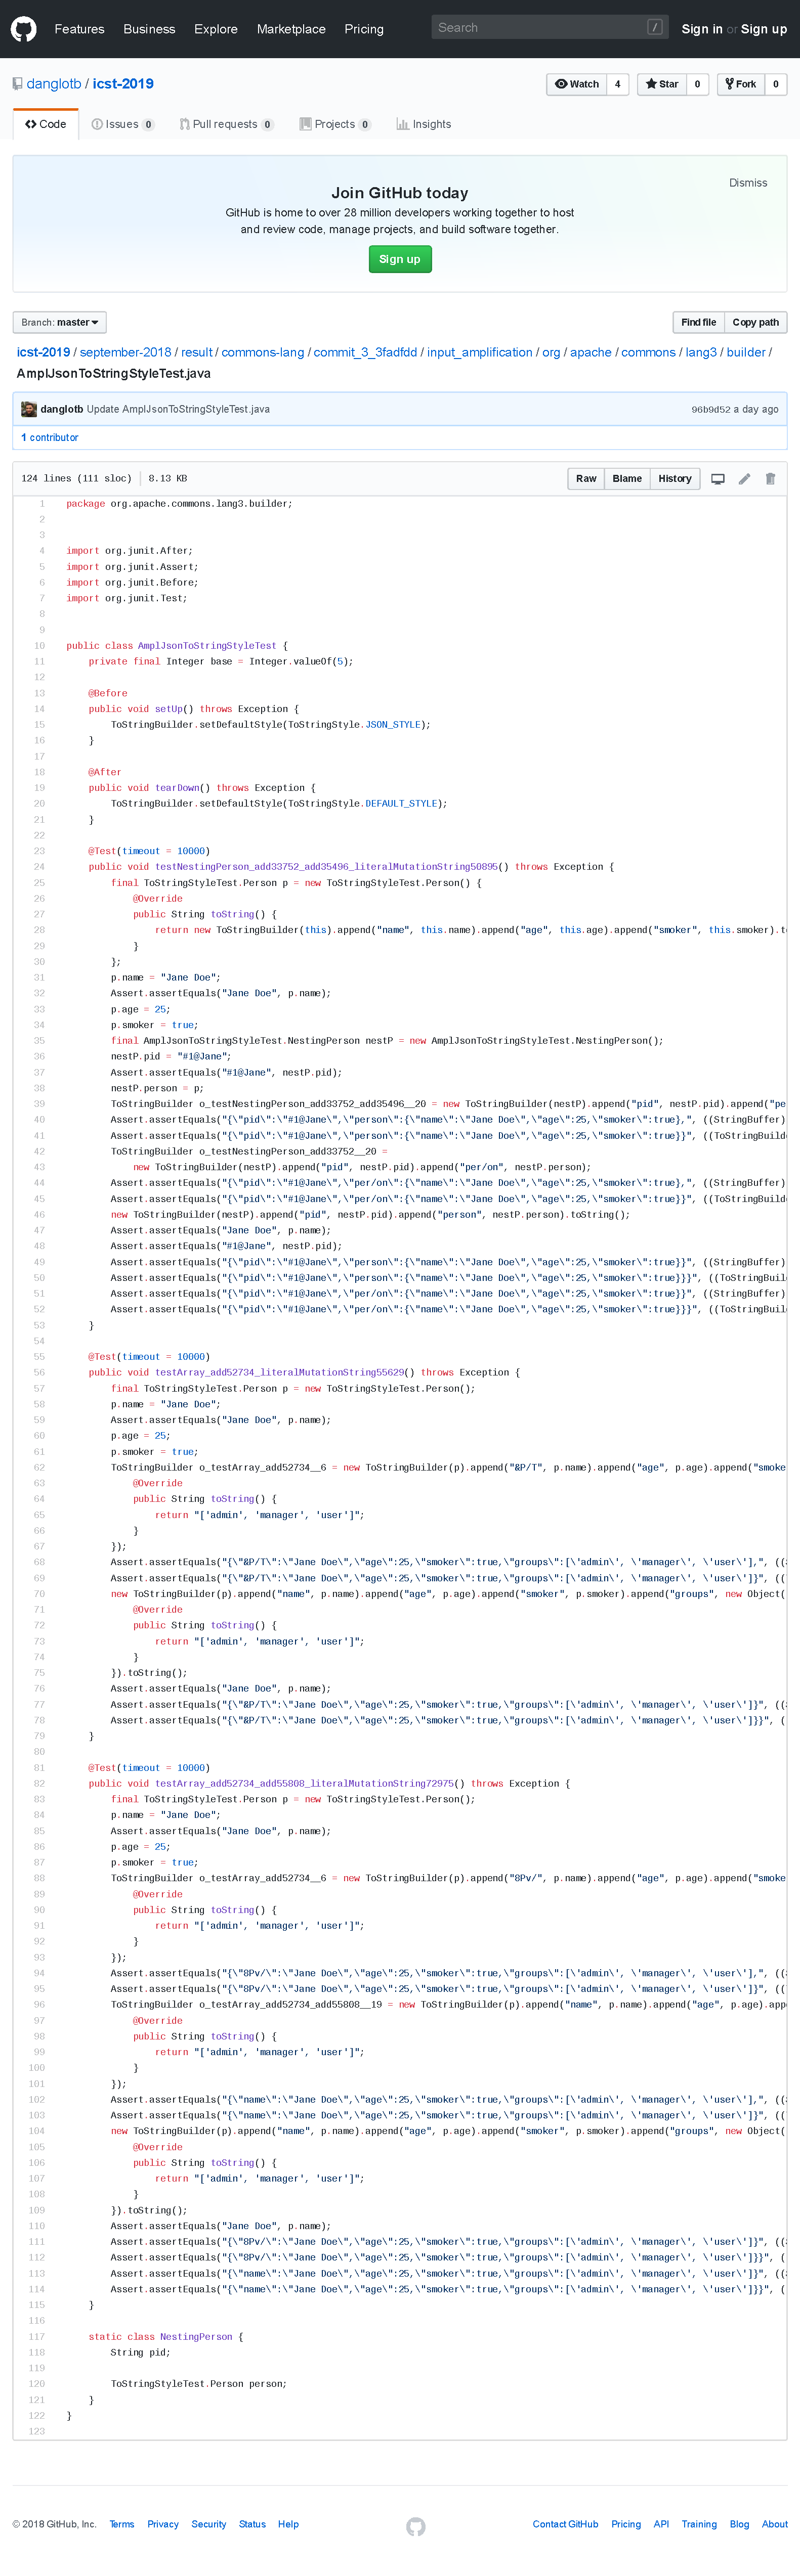
\includegraphics[width=.95\linewidth, trim=3.7cm 46.5cm 9.65cm 38.3cm, clip]{img/amplified/success-ampl-commons-lang.pdf}}
\caption{Test generated by DCI that detects the behavioral change of \textsc{3fadfdd} from commons-lang.}
\label{fig:amplified_commons_lang_success}
\end{figure}

We show in \autoref{fig:amplified_commons_lang_success} 
the resulting amplified test method.
From this test method, DCI generates an amplified test method shown in \autoref{fig:amplified_commons_lang_success}. 
In this generated test, \sbampl applies 2 input transformations: 1 duplication of method call and 1 character replacement in an existing String literal.
The latter transformation is the key transformation: DCI replaced an 's' inside "person" by '/' resulting in "per/on" where "/" is a special character that must be escaped (Line 2). 
Then, DCI generated 11 assertions, based on the modified inputs. 
The amplified test the behavioral change:
in the pre-commit version, the expected value is: \texttt{"\{ ... per/on":\{"name":"Jane Doe" ...\}"} while in the post-commit version it is \texttt{"\{ ... per\textbackslash/on":\{"name":"Jane Doe" ...\}"} (Line 3).
 
%recap RQ2
\begin{mdframed}
Answer to \textbf{RQ1}: Overall, DCI is capable of detecting the behavioral changes in a total of 28/60 commits. Individually, \DCII finds changes in 28/60, while \DCIA in 9/60 commits.
Since \DCII also uses \aampl to generate assertions, all \DCIA's commits are contained in \DCII's. However, the search-based algorithm, through exploration, finds many more behavioral changes, making it more effective albeit at the cost of execution time.
\end{mdframed}

%%%%%%%%%%%%%%%%%%%%%%%%%%%%%%%%%%%%%%%%%%%%%%%%%%%%%
%%%%%%%%%%%%%%%%%%%%%%%%%%%%%%%%%%%%%%%%%%%%%%%%%%%%%
%% RESULTS RQ2 : ITERATION
%%%%%%%%%%%%%%%%%%%%%%%%%%%%%%%%%%%%%%%%%%%%%%%%%%%%%
%%%%%%%%%%%%%%%%%%%%%%%%%%%%%%%%%%%%%%%%%%%%%%%%%%%%%

\subsubsection{\rqiteration}
\label{subsubsec:answerqiteration}

The results are reported in \autoref{tab:overall_result_iteration}
This table can be read as follow:
the first column is the name of the project;
the second column is the commit identifier;
then, the third, fourth, fifth, sixth, seventh and eighth provide the amplification results and execution time for each number of iteration 1, 2, and 3. A \cmark indicates with the number of amplified tests that detect a behavioral change and a \textit{-} denotes that DCI did not succeed in generating a test that detects a change.

% number of detection
Overall, \DCII generates amplified tests that detect 21, 23, and 24 out of 60 behavioral changes for respectively $iteration=1$, $iteration=2$ and $iteration=3$.
The more iteration \DCII does, the more it explores, the more it generates amplified tests that detect the behavioral changes but the more it takes time also.
% difference in number of behavioral changes we detect
When \DCII is used with $iteration=3$, it generates amplified test methods that detect 3 more behavioral changes than when it is used with $iteration=1$ and 1 then when it is used with $iteration=2$. It represents an increase of 14\% and 4\% for respectively $iteration=1$ and $iteration=2$.

% number of test generated
In average, \DCII generates 18, 53, and 116 amplified tests for respectively $iteration=1$, $iteration=2$ and $iteration=3$. 
This number increases by 544\% from $iteration=1$ to $iteration=3$.
This increase is explained by the fact that \DCII explores more with more iteration and thus is able to generate more amplified test methods that detect the behavioral changes.

% time
In average \DCII takes 23, 64, and 105 minutes to perform the amplification for respectively $iteration=1$, $iteration=2$ and $iteration=3$.
This number increases by 356\% from $iteration=1$ to $iteration=3$.

\begin{table*}
\small
\def\arraystretch{1}%  1 is the default, change whatever you need
\setlength\tabcolsep{6pt} % default value: 6pt
\caption{Evaluation of the impact of the number of iteration done by \DCII on 60 commits from 6 open-source projects.}
%\rotvertical{
\label{tab:overall_result_iteration}
\begin{tabular}{l|c|cc|cc|cc}
&
id&
$it=1$&
Time&
$it=2$&
Time&
$it=3$&
Time\\
\midrule
\multirow{11}{*}{\rotverticalinv{commons-io}}
&  c6b8a38  &  0 &  25.0s  &  0  &  62.0s  &  0  &  98.0s\\
&  2736b6f  &  \cmark(1) &  26.1m  &  \cmark(2)  &  44.2m  &  \cmark(12)  &  76.3m\\
&  a4705cc  &  0 &  4.1m  &  0  &  21.1m  &  0  &  38.1m\\
&  f00d97a  &  \cmark(7) &  13.0s  &  \cmark(28)  &  19.0s  &  \cmark(39)  &  27.0s\\
&  3378280  &  \cmark(6) &  15.0s  &  \cmark(10)  &  20.0s  &  \cmark(11)  &  24.0s\\
&  703228a  &  0 &  30.3m  &  0  &  55.1m  &  0  &  71.0m\\
&  a7bd568  &  0 &  28.6m  &  0  &  52.0m  &  0  &  65.2m\\
&  81210eb  &  \cmark(2) &  14.0s  &  \cmark(4)  &  18.0s  &  \cmark(8)  &  23.0s\\
&  57f493a  &  0 &  20.0s  &  0  &  32.0s  &  0  &  54.0s\\
&  5d072ef  &  \cmark(461) &  32.2m  &  \cmark(1014)  &  65.5m  &  \cmark(1538)  &  2.2h\\
\midrule
\rowcolor[HTML]{EFEFEF}
&  total  &  477 &  2.0h  &  1058  &  4.0h  &  1608  &  6.5h\\
\midrule
&  average  &  47.70 &  12.3m  &  105.80  &  24.0m  &  160.80  &  38.8m\\
\midrule
\multirow{11}{*}{\rotverticalinv{commons-lang}}
&  f56931c  &  0 &  0.0s  &  0  &  3.7m  &  0  &  8.5m\\
&  87937b2  &  0 &  3.5m  &  0  &  10.5m  &  0  &  18.1m\\
&  09ef69c  &  0 &  97.0s  &  0  &  21.0m  &  0  &  98.8m\\
&  3fadfdd  &  \cmark(1) &  2.0m  &  \cmark(1)  &  9.3m  &  \cmark(4)  &  17.2m\\
&  e7d16c2  &  \cmark(3) &  111.0s  &  \cmark(2)  &  8.4m  &  \cmark(2)  &  15.1m\\
&  50ce8c4  &  \cmark(61) &  38.0s  &  \cmark(97)  &  78.0s  &  \cmark(135)  &  2.0m\\
&  2e9f3a8  &  0 &  11.4m  &  0  &  35.0m  &  0  &  66.5m\\
&  c8e61af  &  0 &  16.0s  &  0  &  16.0s  &  0  &  16.0s\\
&  d8ec011  &  0 &  36.0s  &  0  &  68.0s  &  0  &  2.3m\\
&  7d061e3  &  0 &  79.0s  &  0  &  5.8m  &  0  &  11.4m\\
\midrule
\rowcolor[HTML]{EFEFEF}
&  total  &  65 &  23.3m  &  100  &  96.4m  &  141  &  4.0h\\
\midrule
&  average  &  6.50 &  2.3m  &  10.00  &  9.6m  &  14.10  &  24.0m\\
\midrule
\multirow{11}{*}{\rotverticalinv{gson}}
&  b1fb9ca  &  0 &  14.6m  &  0  &  51.0m  &  0  &  92.5m\\
&  7a9fd59  &  \cmark(7) &  33.0s  &  \cmark(48)  &  73.0s  &  \cmark(108)  &  2.1m\\
&  03a72e7  &  0 &  30.2m  &  0  &  102.3m  &  0  &  3.2h\\
&  74e3711  &  0 &  6.0s  &  0  &  11.0s  &  0  &  16.0s\\
&  ada597e  &  0 &  61.0s  &  0  &  4.9m  &  0  &  8.7m\\
&  a300148  &  0 &  45.2m  &  \cmark(4)  &  2.6h  &  \cmark(6)  &  4.9h\\
&  9a24219  &  0 &  10.8m  &  0  &  28.4m  &  0  &  48.9m\\
&  9e6f2ba  &  0 &  79.0s  &  0  &  4.5m  &  \cmark(2)  &  8.5m\\
&  44cad04  &  \cmark(4) &  21.0s  &  \cmark(21)  &  30.0s  &  \cmark(37)  &  40.0s\\
&  b2c00a3  &  0 &  31.5m  &  0  &  111.8m  &  0  &  3.6h\\
\midrule
\rowcolor[HTML]{EFEFEF}
&  total  &  11 &  2.3h  &  73  &  7.7h  &  153  &  14.4h\\
\midrule
&  average  &  1.10 &  13.6m  &  7.30  &  46.0m  &  15.30  &  86.5m\\
\midrule
\multirow{11}{*}{\rotverticalinv{jsoup}}
&  426ffe7  &  \cmark(126) &  5.4m  &  \cmark(172)  &  19.2m  &  \cmark(198)  &  33.6m\\
&  a810d2e  &  0 &  90.0s  &  0  &  13.9m  &  0  &  26.6m\\
&  6be19a6  &  0 &  8.1m  &  0  &  39.7m  &  0  &  67.7m\\
&  e38dfd4  &  0 &  117.0s  &  0  &  6.3m  &  0  &  12.5m\\
&  e9feec9  &  0 &  20.0s  &  0  &  50.0s  &  0  &  95.0s\\
&  0f7e0cc  &  \cmark(1) &  2.4h  &  \cmark(7)  &  6.8h  &  \cmark(36)  &  11.8h\\
&  2c4e79b  &  0 &  7.1m  &  0  &  34.1m  &  0  &  4.7h\\
&  e5210d1  &  0 &  45.0s  &  0  &  2.3m  &  0  &  4.9m\\
&  df272b7  &  0 &  43.0s  &  0  &  2.2m  &  0  &  4.6m\\
&  3676b13  &  \cmark(6) &  21.4m  &  \cmark(35)  &  2.9h  &  \cmark(52)  &  6.8h\\
\midrule
\rowcolor[HTML]{EFEFEF}
&  total  &  133 &  3.2h  &  214  &  11.6h  &  286  &  25.8h\\
\midrule
&  average  &  13.30 &  19.4m  &  21.40  &  69.8m  &  28.60  &  2.6h\\
\midrule
\multirow{11}{*}{\rotverticalinv{mustache.java}}
&  a1197f7  &  \cmark(28) &  5.9h  &  \cmark(124)  &  8.4h  &  \cmark(204)  &  10.1h\\
&  8877027  &  0 &  30.5m  &  0  &  58.4m  &  0  &  100.2m\\
&  d8936b4  &  0 &  3.2m  &  0  &  4.8m  &  0  &  84.2m\\
&  88718bc  &  \cmark(13) &  78.0s  &  \cmark(85)  &  2.5m  &  \cmark(149)  &  3.7m\\
&  339161f  &  \cmark(143) &  115.9m  &  \cmark(699)  &  4.1h  &  \cmark(1312)  &  5.8h\\
&  774ae7a  &  \cmark(18) &  2.7m  &  \cmark(65)  &  4.7m  &  \cmark(124)  &  6.8m\\
&  94847cc  &  \cmark(122) &  5.3h  &  \cmark(580)  &  10.4h  &  \cmark(2509)  &  21.4h\\
&  eca08ca  &  0 &  8.1m  &  0  &  24.3m  &  0  &  41.8m\\
&  6d7225c  &  0 &  7.9m  &  0  &  26.8m  &  0  &  40.1m\\
&  8ac71b7  &  \cmark(2) &  2.7m  &  \cmark(48)  &  3.8m  &  \cmark(124)  &  5.6m\\
\midrule
\rowcolor[HTML]{EFEFEF}
&  total  &  326 &  14.0h  &  1601  &  25.0h  &  4422  &  42.0h\\
\midrule
&  average  &  32.60 &  84.3m  &  160.10  &  2.5h  &  442.20  &  4.2h\\
\midrule
\multirow{11}{*}{\rotverticalinv{xwiki-commons}}
&  ffc3997  &  0 &  19.0s  &  0  &  18.0s  &  0  &  18.0s\\
&  ced2635  &  0 &  8.0m  &  0  &  31.8m  &  0  &  2.5h\\
&  10841b1  &  0 &  56.2m  &  0  &  2.9h  &  0  &  3.4h\\
&  848c984  &  0 &  18.0s  &  0  &  17.0s  &  0  &  18.0s\\
&  adfefec  &  \cmark(22) &  3.5m  &  \cmark(57)  &  9.9m  &  \cmark(3)  &  14.9m\\
&  d3101ae  &  \cmark(9) &  11.6m  &  \cmark(12)  &  28.2m  &  \cmark(31)  &  41.4m\\
&  a0e8b77  &  \cmark(10) &  12.0m  &  \cmark(17)  &  28.2m  &  \cmark(60)  &  42.1m\\
&  78ff099  &  \cmark(4) &  2.6m  &  \cmark(4)  &  4.6m  &  \cmark(4)  &  6.6m\\
&  1b79714  &  0 &  4.0m  &  0  &  10.7m  &  0  &  17.9m\\
&  6dc9059  &  0 &  4.0m  &  0  &  10.8m  &  0  &  20.5m\\
\midrule
\rowcolor[HTML]{EFEFEF}
&  total  &  45 &  102.8m  &  90  &  4.9h  &  98  &  8.2h\\
\midrule
&  average  &  4.50 &  10.3m  &  9.00  &  29.7m  &  9.80  &  49.5m\\
\midrule
\midrule
&  total  &  23(1057) &  23.7h  &  24(3136)  &  54.9h  &  25(6708)  &  100.9h\\
\bottomrule
\end{tabular}
%}
\end{table*}

\paragraph{Impact of the randomness}

The number of amplified test methods obtained by the different seeds are reported in \autoref{tab:overall_result_seeds}.
The result of the Kruskal-Wallis test is:  p-value=0.96.
$p-value>\alpha$ which means that we keep the null hypothesis: 
The population median of all of the groups are equal.
This means that, in general, the choice of the seeds has not a significant impact of the overall result of DCI.

\begin{table*}
\small
\def\arraystretch{.5}%  1 is the default, change whatever you need
\setlength\tabcolsep{3pt} % default value: 6pt
\caption{Number of amplified test methods obtained by DCI for 10 different seeds. The first column is the id of the commit. The second column is the result obtained with the default seed, used during the evaluation for \rqdetection. The ten following columns are the result obtained for the 10 different seeds.}
\label{tab:overall_result_seeds}
\begin{tabular}{l|c|llllllllll}
&id&0&1&2&3&4&5&6&7&8&9\\
\hline
\multirow{11}{*}{\rotvertical{commons-io}}
 & c6b8a38 & - & - & - & - & - & - & - & - & - & -\\
 & 2736b6f & 1 & 1 & - & 2 & 1 & 1 & 2 & 1 & - & -\\
 & a4705cc & - & - & - & - & - & - & - & - & - & -\\
 & f00d97a & 7 & 7 & 7 & 7 & 7 & 7 & 7 & 7 & 7 & 7\\
 & 3378280 & 6 & 6 & 6 & 6 & 6 & 6 & 6 & 6 & 6 & 6\\
 & 703228a & - & - & - & - & - & 2 & - & 1 & - & -\\
 & a7bd568 & - & - & - & - & - & 2 & - & 1 & - & -\\
 & 81210eb & 2 & 2 & 2 & 2 & 2 & 2 & 2 & 2 & 2 & 2\\
 & 57f493a & - & - & - & - & - & - & - & - & - & -\\
 & 5d072ef & 464 & 462 & 463 & 463 & 461 & 462 & 465 & 460 & 463 & 462\\
\hline
\multirow{11}{*}{\rotvertical{commons-lang}}
 & f56931c & - & - & - & - & 1 & - & 1 & 1 & 1 & 1\\
 & 87937b2 & - & - & - & - & - & - & - & - & - & -\\
 & 09ef69c & - & - & - & - & - & - & - & - & - & -\\
 & 3fadfdd & 1 & - & 2 & 3 & 3 & 2 & 1 & - & - & 1\\
 & e7d16c2 & - & 1 & - & - & 1 & 1 & - & 1 & 1 & 1\\
 & 50ce8c4 & 61 & 63 & 62 & 57 & 58 & 60 & 61 & 62 & 63 & 61\\
 & 2e9f3a8 & - & - & - & - & - & - & - & - & - & -\\
 & c8e61af & - & - & - & - & - & - & - & - & - & -\\
 & d8ec011 & - & - & - & - & - & - & - & - & - & -\\
 & 7d061e3 & - & - & - & - & - & - & - & - & - & -\\
\hline
\multirow{11}{*}{\rotvertical{gson}}
 & b1fb9ca & - & - & - & - & - & - & - & - & - & -\\
 & 7a9fd59 & 7 & 7 & 7 & 7 & 7 & 7 & 7 & 7 & 7 & 7\\
 & 03a72e7 & - & - & - & - & - & - & - & - & 0 & 3\\
 & 74e3711 & - & - & - & - & - & - & - & - & - & -\\
 & ada597e & - & - & - & - & - & - & - & - & - & -\\
 & a300148 & - & - & - & - & - & - & - & - & - & -\\
 & 9a24219 & - & - & - & - & - & - & - & - & - & -\\
 & 9e6f2ba & - & - & - & - & - & - & - & - & - & -\\
 & 44cad04 & 5 & 4 & 6 & 4 & 4 & 4 & 4 & 4 & 3 & 5\\
 & b2c00a3 & - & - & - & - & - & - & - & - & - & -\\
\hline
\multirow{11}{*}{\rotvertical{jsoup}}
 & 426ffe7 & 125 & 125 & 123 & 126 & 126 & 127 & 123 & 121 & 119 & 121\\
 & a810d2e & - & - & - & - & - & - & - & - & - & -\\
 & 6be19a6 & - & - & - & - & - & - & - & - & - & -\\
 & e38dfd4 & - & - & - & - & - & - & - & - & - & -\\
 & e9feec9 & - & - & - & - & - & 1 & - & 1 & - & -\\
 & 0f7e0cc & - & - & 1 & 1 & - & 1 & 1 & - & 1 & -\\
 & 2c4e79b & - & - & - & - & - & - & - & - & - & -\\
 & e5210d1 & - & - & - & - & - & - & - & - & - & -\\
 & df272b7 & - & - & - & - & - & - & - & - & - & -\\
 & 3676b13 & 3 & 6 & 2 & 3 & 4 & 1 & 1 & 1 & 1 & -\\
\hline
\multirow{11}{*}{\rotvertical{mustache.java}}
 & a1197f7 & 22 & - & - & - & - & - & - & - & - & -\\
 & 8877027 & - & - & - & - & - & - & - & - & - & -\\
 & d8936b4 & - & - & - & - & - & - & - & - & - & -\\
 & 88718bc & 12 & 11 & 13 & 13 & 11 & 13 & 12 & 12 & 12 & 12\\
 & 339161f & 135 & 146 & - & - & - & - & 138 & - & - & 144\\
 & 774ae7a & 23 & 18 & 3 & 17 & 18 & 15 & 16 & 19 & 17 & 20\\
 & 94847cc & - & - & 112 & - & 61 & 72 & 57 & 40 & 42 & 37\\
 & eca08ca & - & - & - & - & - & - & - & - & - & -\\
 & 6d7225c & - & - & - & - & - & - & - & - & - & -\\
 & 8ac71b7 & 2 & 2 & 2 & 2 & 2 & 2 & 2 & 2 & 2 & 2\\
\hline
\multirow{11}{*}{\rotvertical{xwiki-commons}}
 & ffc3997 & - & - & - & - & - & - & - & - & - & -\\
 & ced2635 & - & - & - & - & - & - & - & - & - & -\\
 & 10841b1 & - & - & - & - & - & - & - & - & - & -\\
 & 848c984 & - & - & - & - & - & - & - & - & - & -\\
 & adfefec & 1 & 1 & 1 & 1 & 1 & 1 & 1 & 1 & 1 & 1\\
 & d3101ae & 18 & 15 & 13 & 14 & 15 & 14 & - & 15 & 12 & 15\\
 & a0e8b77 & 19 & - & 14 & 15 & 17 & 15 & 16 & 16 & 13 & 16\\
 & 78ff099 & 4 & 4 & 4 & 4 & 4 & 4 & 4 & 4 & 4 & 4\\
 & 1b79714 & - & - & - & - & - & - & - & - & - & -\\
 & 6dc9059 & - & - & - & - & - & - & - & - & - & -\\
\hline
\end{tabular}
\end{table*}

%recap RQ2
\begin{mdframed}
Answer to \textbf{RQ2}: \DCII detects  21, 23, and 24 behavioral changes out of 60 for respectively $iteration=1$, $iteration=2$ and $iteration=3$.
The number of iteration done by \DCII impacts the number of behavioral changes detected, the number of amplified test methods obtained and the execution time.
\end{mdframed}

%%%%%%%%%%%%%%%%%%%%%%%%%%%%%%%%%%%%%%%%%%%%%%%%%%%%%
%%%%%%%%%%%%%%%%%%%%%%%%%%%%%%%%%%%%%%%%%%%%%%%%%%%%%
%% RESULTS RQ3
%%%%%%%%%%%%%%%%%%%%%%%%%%%%%%%%%%%%%%%%%%%%%%%%%%%%%
%%%%%%%%%%%%%%%%%%%%%%%%%%%%%%%%%%%%%%%%%%%%%%%%%%%%%

\subsubsection{\rqselection}
\label{subsubsec:answerq3}

To answer \textbf{RQ3}, there is no quantitative approach to take, because there is no ground truth data or metrics to optimize. 
Per our protocol described in \autoref{subsec:protocol}, we answer this question based on manual analysis:
we randomly selected 1 commit per project, and we analyzed the relevance of the selected tests for amplification.

In order to give an intuition of what we consider as a relevant test selection for amplification, let us look at an example. 
If \texttt{TestX} is selected for amplification, following a change to method \texttt{X}, we consider this as relevant. The key is that DCI will generate an amplified test \texttt{TestX'} that is a variant of \texttt{TestX}, and, consequently, the developer will directly get the intention of the new test \texttt{TestX'} and what behavioral change it detects.

\textsc{Commons-io\#c6b8a38}\footnote{\url{https://github.com/apache/commons-io/commit/c6b8a38}}: our test selection returns 3 test methods: \texttt{testContentEquals}, \texttt{testCopyURLToFileWithTimeout} and \texttt{testCopyURLToFile} from the same test class: \texttt{FileUtilsTestCase}.
The considered commit modifies the method \texttt{copyToFile} from \texttt{FileUtils}. 
Two test methods out 3 (\texttt{testCopyURLToFileWithTimeout} and \texttt{testCopyURLToFile}) there is a link between the changed file and the intention of tests to be amplified. 
The selection is thus considered relevant.

\textsc{Commons-lang\#f56931c}\footnote{\url{https://github.com/apache/commons-lang/commit/f56931c}}: our test selection returns 39 test methods from 5 test classes: \texttt{FastDateFormat\_ParserTest}, \texttt{FastDateParserTest}, \texttt{DateUtilsTest}, \texttt{FastDateParser\_TimeZoneStrategyTest} and \texttt{FastDateParser\_MoreOrLessTest}.
This commit modifies the behavior of two methods: \texttt{simpleQuote} and \texttt{setCalendar} of class \texttt{FastDateParser}.
Our manual analysis reveals two intentions:
1) test behaviors related to parsing, 
1) test behaviors related to dates.
While this is meaningful, a set of 39 methods is clearly not a focused selection, not as focused as for the previous example.
It is considered as an half-success.

 \textsc{Gson\#9e6f2ba}\footnote{\url{https://github.com/google/gson/commit/9e6f2ba}}: our test selection returns 9 test methods from 5 different test classes.
 Three out of those five classes \texttt{JsonElementReaderTest}, \texttt{JsonReaderPathTest} and \texttt{JsonParserTest} relate to the class modified in the commit(\texttt{JsonTreeReader}).
The selection is thus considered relevant but unfocused.

 \textsc{Jsoup\#e9feec9}\footnote{\url{https://github.com/jhy/jsoup/commit/e9feec9}}, our test selection returns the 4 test methods defined in the \texttt{XmlTreeBuilderTest} class : \texttt{caseSensitiveDeclaration}, \texttt{handlesXmlDeclarationAsDeclaration}, \texttt{testDetectCharsetEncodingDeclaration} and \texttt{testParseDeclarationAttributes}.
 The commit modifies the behavior of the class \texttt{XmlTreeBuilder}.
Here, the test selection is relevant.
Actually, the ground-truth manual test added in the commit is also in the \texttt{XmlTreeBuilderTest} class.
If DCI proposes a new test there to capture the behavioral change, the developer will understand its relevance and its relation to the change.

\textsc{Mustache.java\#88718bc}\footnote{\url{https://github.com/spullara/mustache.java/commit/88718bc}}, our test selection returns the \texttt{testInvalidDelimiters} test method defined in the \texttt{com.github.mustachejava.InterpreterTest} test class.
The commit improves an error message when an invalid delimiter is used.
Here, the test selection is relevant since it selected \texttt{testInvalidDelimiters} which is the dedicated test to the usage of the test invalid delimiters.
This ground-truth test method is also in the test class \texttt{com.github.mustachejava.InterpreterTest}.

\textsc{Xwiki-commons\#848c984}\footnote{\url{https://github.com/xwiki/xwiki-commons/commit/848c984}} our test selection returns a single test method \texttt{createReference} from test class \texttt{XWikiDocumentTest}.
The main modification of this commit is on class \texttt{XWikiDocument}.
Since \texttt{XWikiDocumentTest} is the test class dedicated to \texttt{XWikiDocument}, this is considered as a success.

\begin{mdframed}
Answer to \textbf{RQ3}: 
In 4 out of 6 of the manually analyzed cases, the tests selected to be amplified relate, semantically, to the modified application code. 
In the 2 remaining cases, we selected over and above the tests to be amplified.
That is, we select tests whose intention is semantically pertinent to the change, but we also include tests that are not.
%the test intention is captured but not focused.
%, the test class name, method name and initialization code 
%This indicates that in the selected tests by DCI give the right context for the developer to understand what behavioral change is specified.
However, even in this case, DCI's test selection provides developers with important and targeted context to better understand the behavioral change at hand.
\end{mdframed}


%%%%%%%%%%%%%%%%%%%%%%%%%%%%%%%%%%%%%%%%%%%%%%%%%%%%%
%%%%%%%%%%%%%%%%%%%%%%%%%%%%%%%%%%%%%%%%%%%%%%%%%%%%%
%% RESULTS RQ4
%%%%%%%%%%%%%%%%%%%%%%%%%%%%%%%%%%%%%%%%%%%%%%%%%%%%%
%%%%%%%%%%%%%%%%%%%%%%%%%%%%%%%%%%%%%%%%%%%%%%%%%%%%%
\subsubsection{\rqhuman}
\label{subsubsec:answerq4}

When DCI generates an amplified test method that detects the behavioral change, we can compare it to the ground truth version (the test added in the commit) to see whether it captures the same behavioral change.
For each project, we select 1 successful application of DCI, and we compare the DCI test against the human test.
If they capture the same behavioral change, it means they have the same intention and we consider the amplification a success.

%%% COMMONS IO

\textsc{commons-io\#81210eb}\footnote{\url{https://github.com/apache/commons-io/commit/81210eb}}: This commit modifies the behavior of the \texttt{read()} method in \texttt{BoundedReader}.
\autoref{fig:ampl_commons-io} shows the test generated by \DCII.
This test is amplified from the existing \texttt{readMulti} test, which indicates that the intention is to test the read functionality.
The first line of the test is the construction of a \texttt{BoundedReader} object which is also the class modified by the commit.
\DCII modified the second parameter of the constructor call (transformed $3$ into a $0$) and generated two assertions (only 1 is shown).
The first assertion, associated to the new test input, captures the behavioral difference.
Overall, this can be considered as a successful amplication.

\begin{figure}[h]
\centering
\fbox{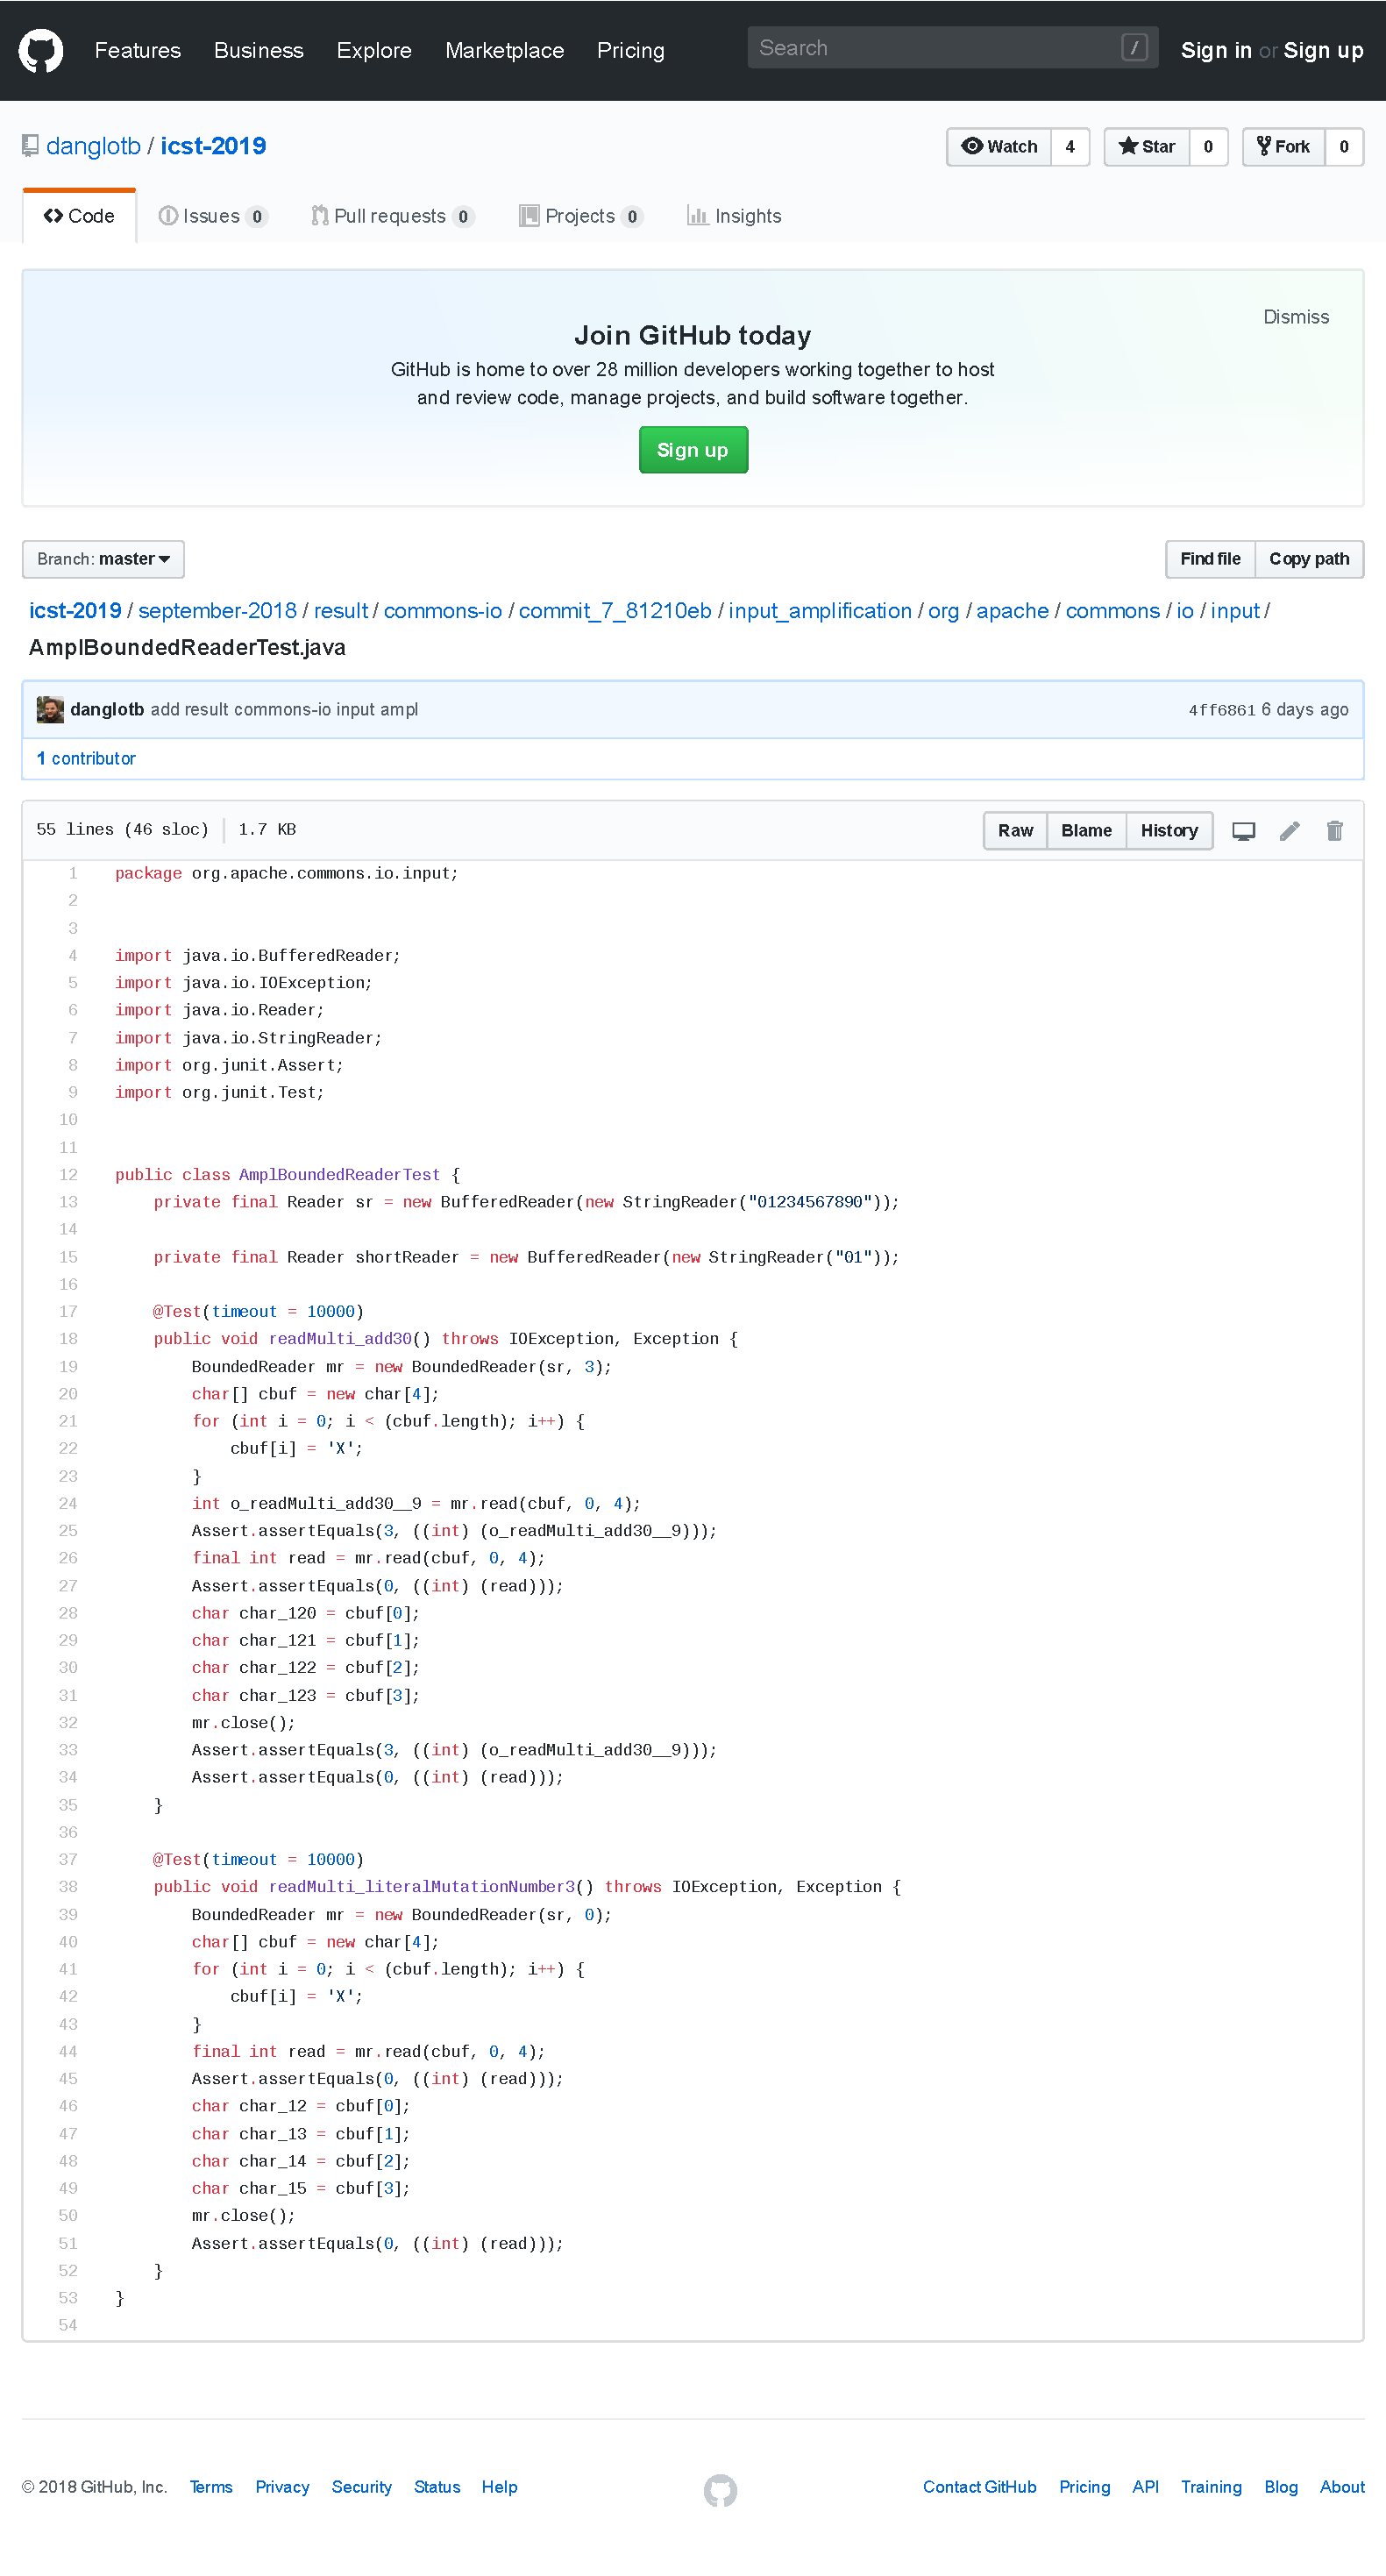
\includegraphics[width=.97\linewidth, trim=3.6cm 9.3cm 14.7cm 36.8cm, clip]{img/amplified/ampl-commons-io.pdf}}
\caption{Test generated by \DCII that detects the behavioral change introduced by commit \textsc{81210eb} in commons-io.}
\label{fig:ampl_commons-io}
\end{figure}

Now, let us look at the human test contained in the commit, shown in \autoref{fig:diff_commons-io}.
It captures the behavioral change with the timeout (the test timeouts on the pre-commit version and goes fast enough on the post-commit version). 
Furthermore, it only indirectly calls the changed method through a call to \texttt{readLine}.

In this case, the DCI test can be considered better than the developer test because
1) it relies on assertions and not on timeouts, and
2) it directly calls the changed method (\texttt{read}) instead of indirectly. 

\begin{figure}[h]
\centering
\fbox{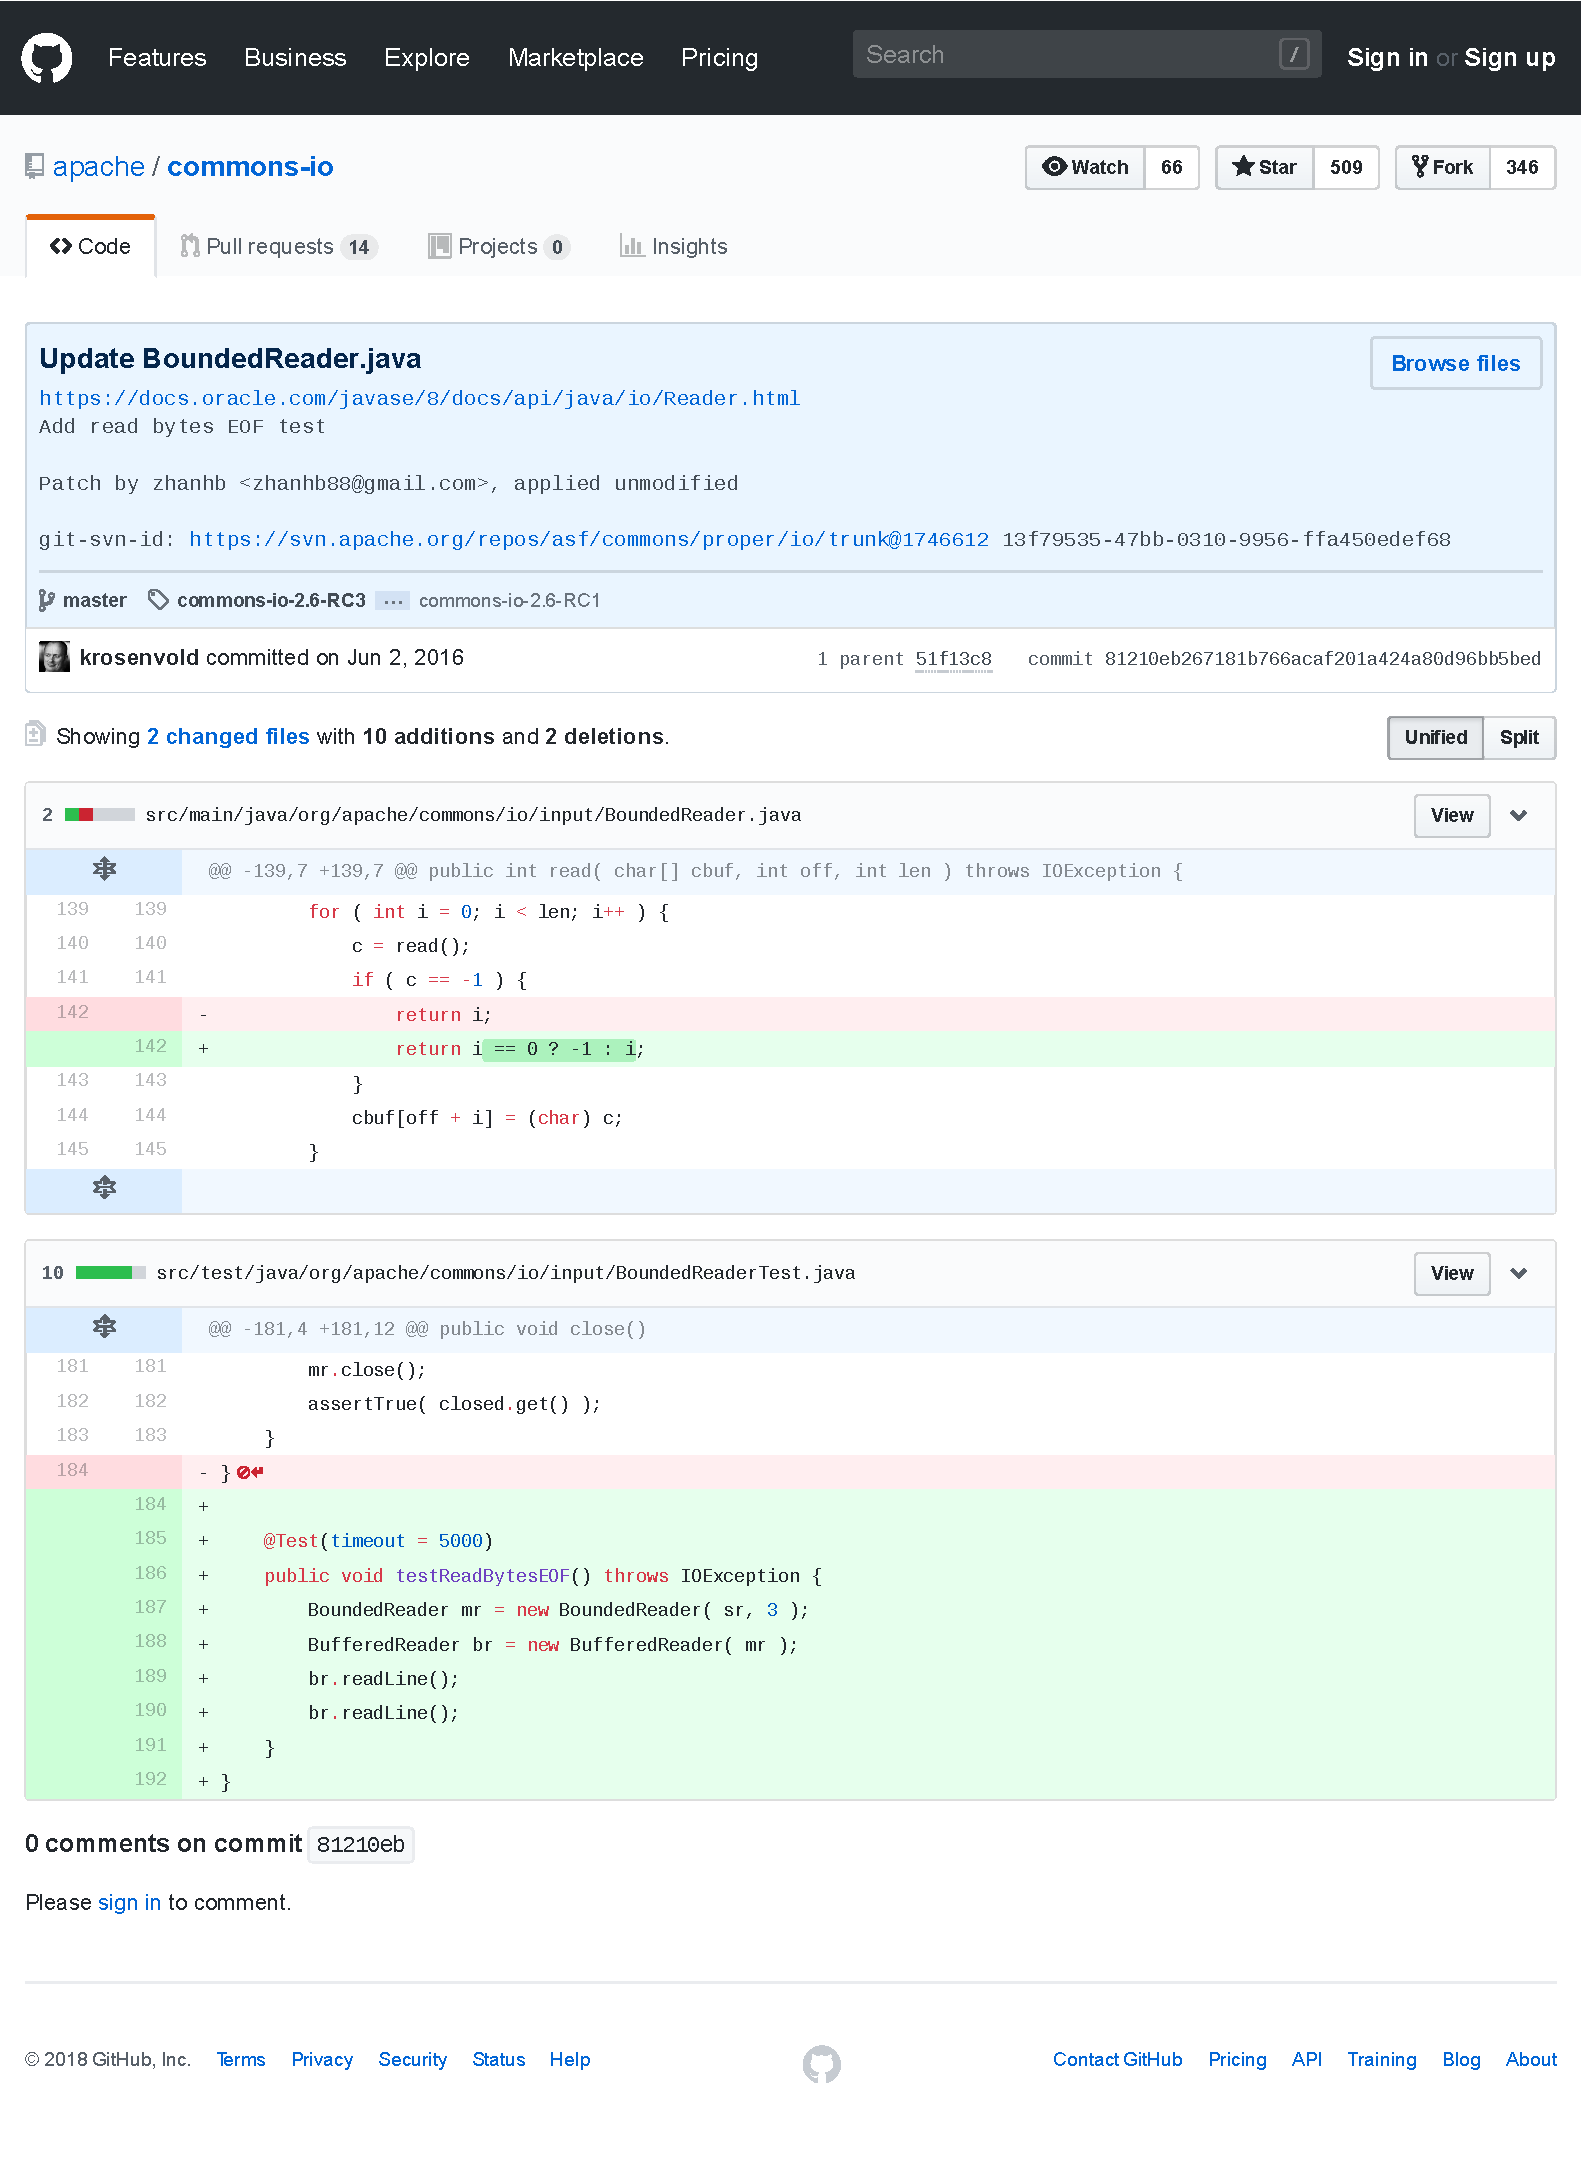
\includegraphics[width=.97\linewidth, trim=4cm 6.7cm 12.6cm 25.8cm, clip]{img/diff/diff-commons-io.pdf}}
\caption{Developer test for commit \textsc{81210eb} of commons-io.}
\label{fig:diff_commons-io}
\end{figure}


%%% COMMONS LANG
\textsc{commons-lang\#e7d16c2}\footnote{\url{https://github.com/apache/commons-lang/commit/e7d16c2}}: this commit escapes special characters before adding them to a \texttt{StringBuffer}.
\autoref{fig:ampl_commons-lang} shows the amplified test method obtained by \DCII.
The assertion at the bottom of the excerpt is the one that detects the behavioral change.
This assertion compares the content of the \texttt{StringBuilder} against an expected string.
In the pre-commit version, no special character is escaped, \eg '\textbackslash n'.
In the post-commit version, the DCI test fails since the code now escapes the special character \textbackslash.

\begin{figure}[h]
\centering
\fbox{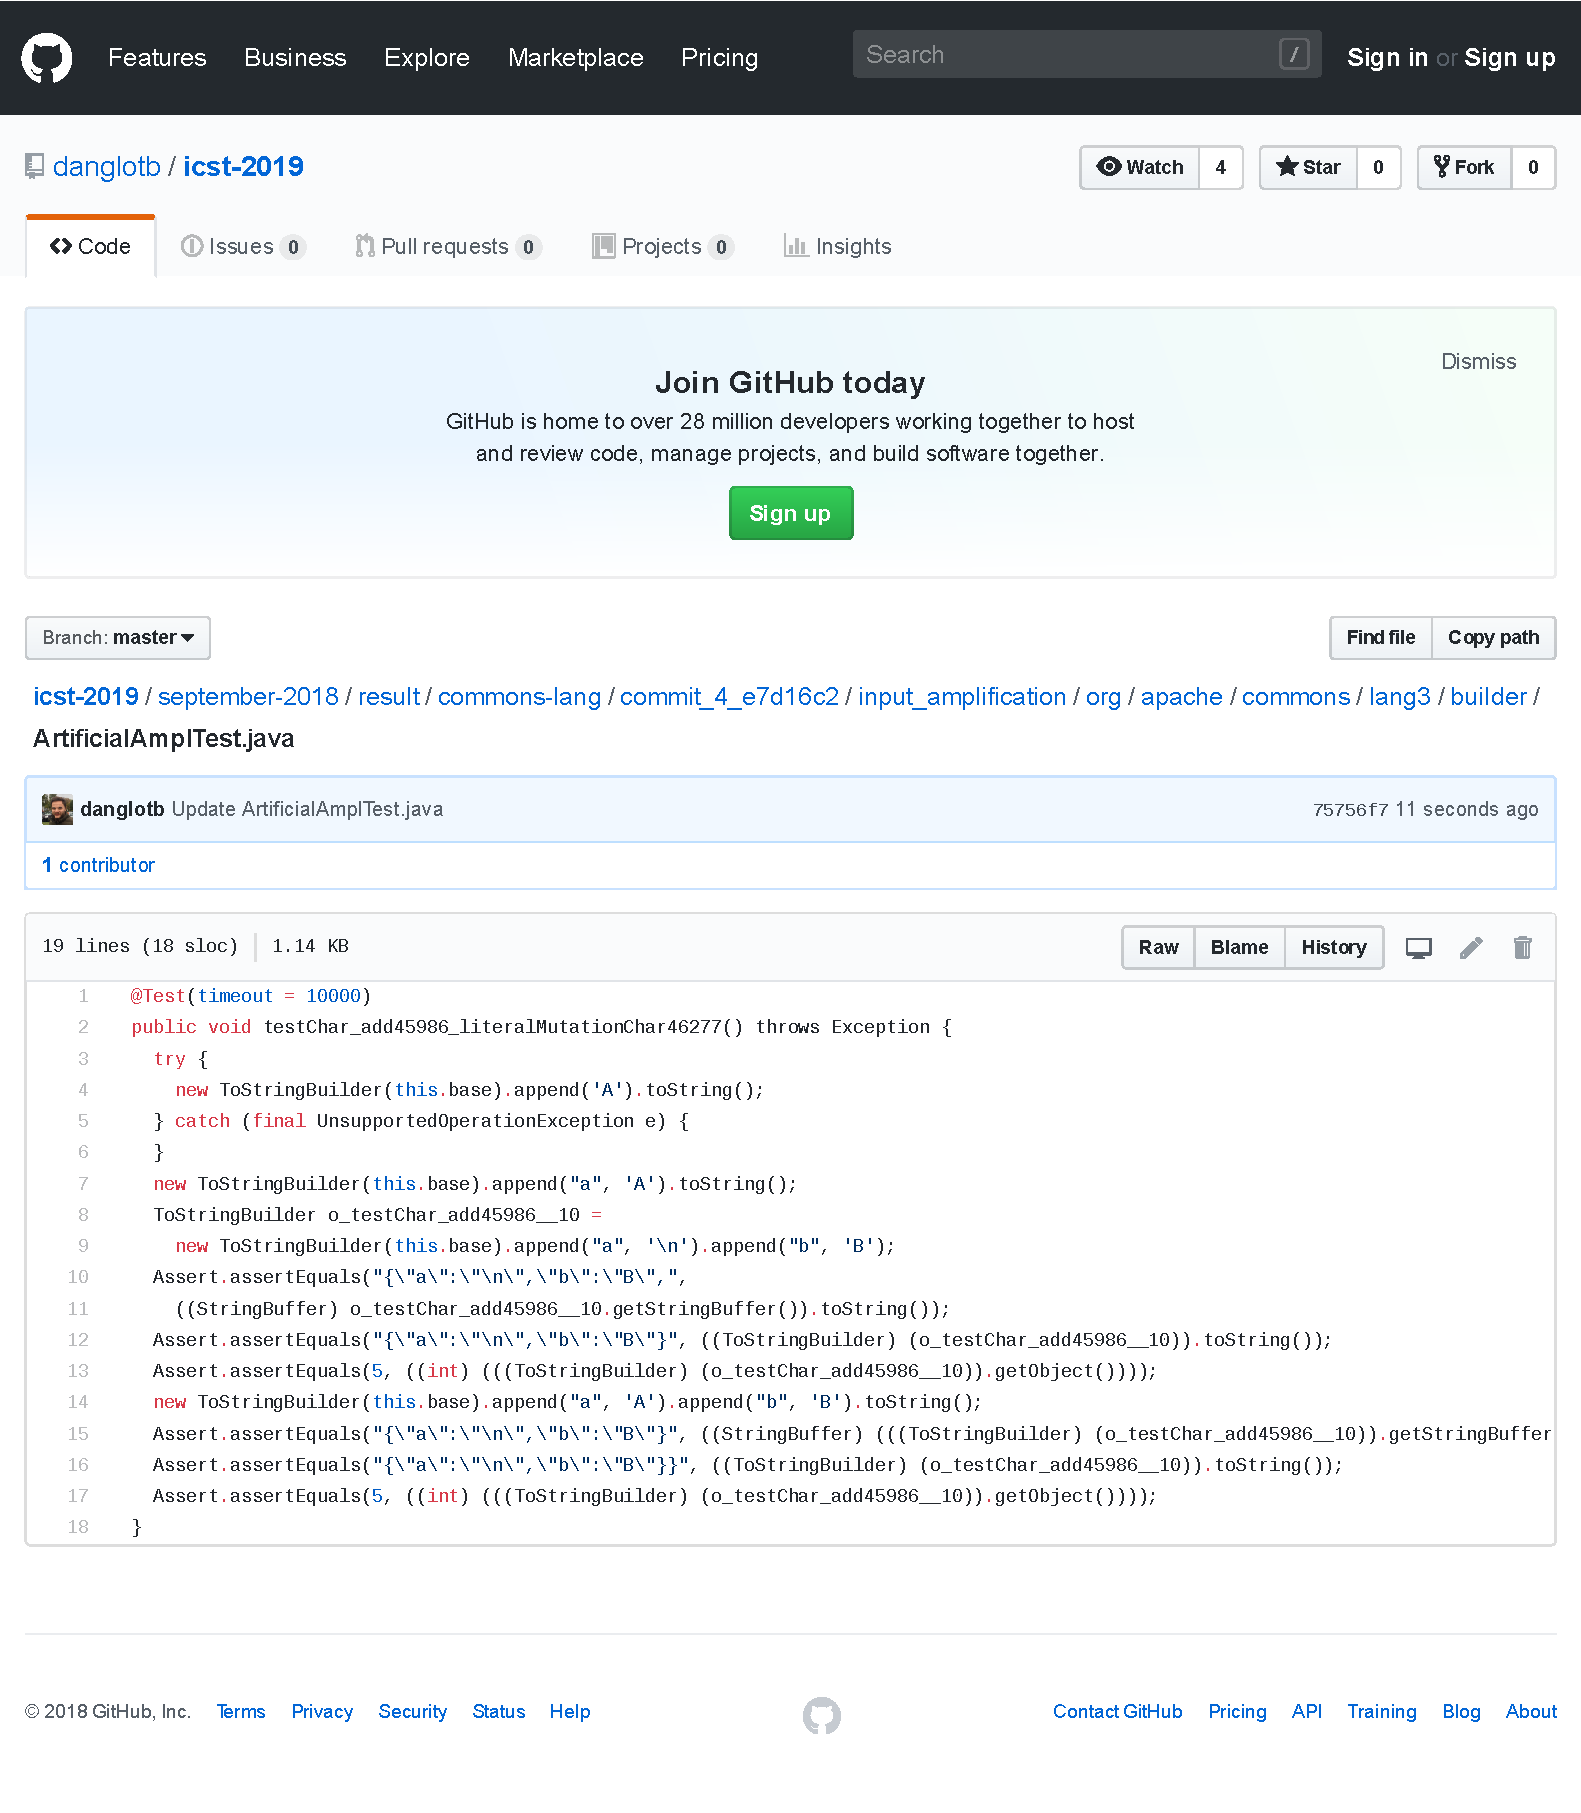
\includegraphics[width=.97\linewidth, trim=2.6cm 8.35cm 10.8cm 20.85cm, clip ]{img/amplified/ampl-commons-lang.pdf}}
\caption{Test generated by \DCII that detects the behavioral change of \textsc{e7d16c2} in commons-lang.}
\label{fig:ampl_commons-lang}
\end{figure}

Let's have a look to the human test method shown in \autoref{fig:diff_commons-lang}.
Here, the developer specified the new escaping mechanism with 5 different inputs.
%
The main difference between the human test and the amplified test is that the human test is more readable and uses 5 different inputs.
However, the amplified test generated by DCI is valid since it detects the behavioral change correctly.

\begin{figure}[h]
\centering
\fbox{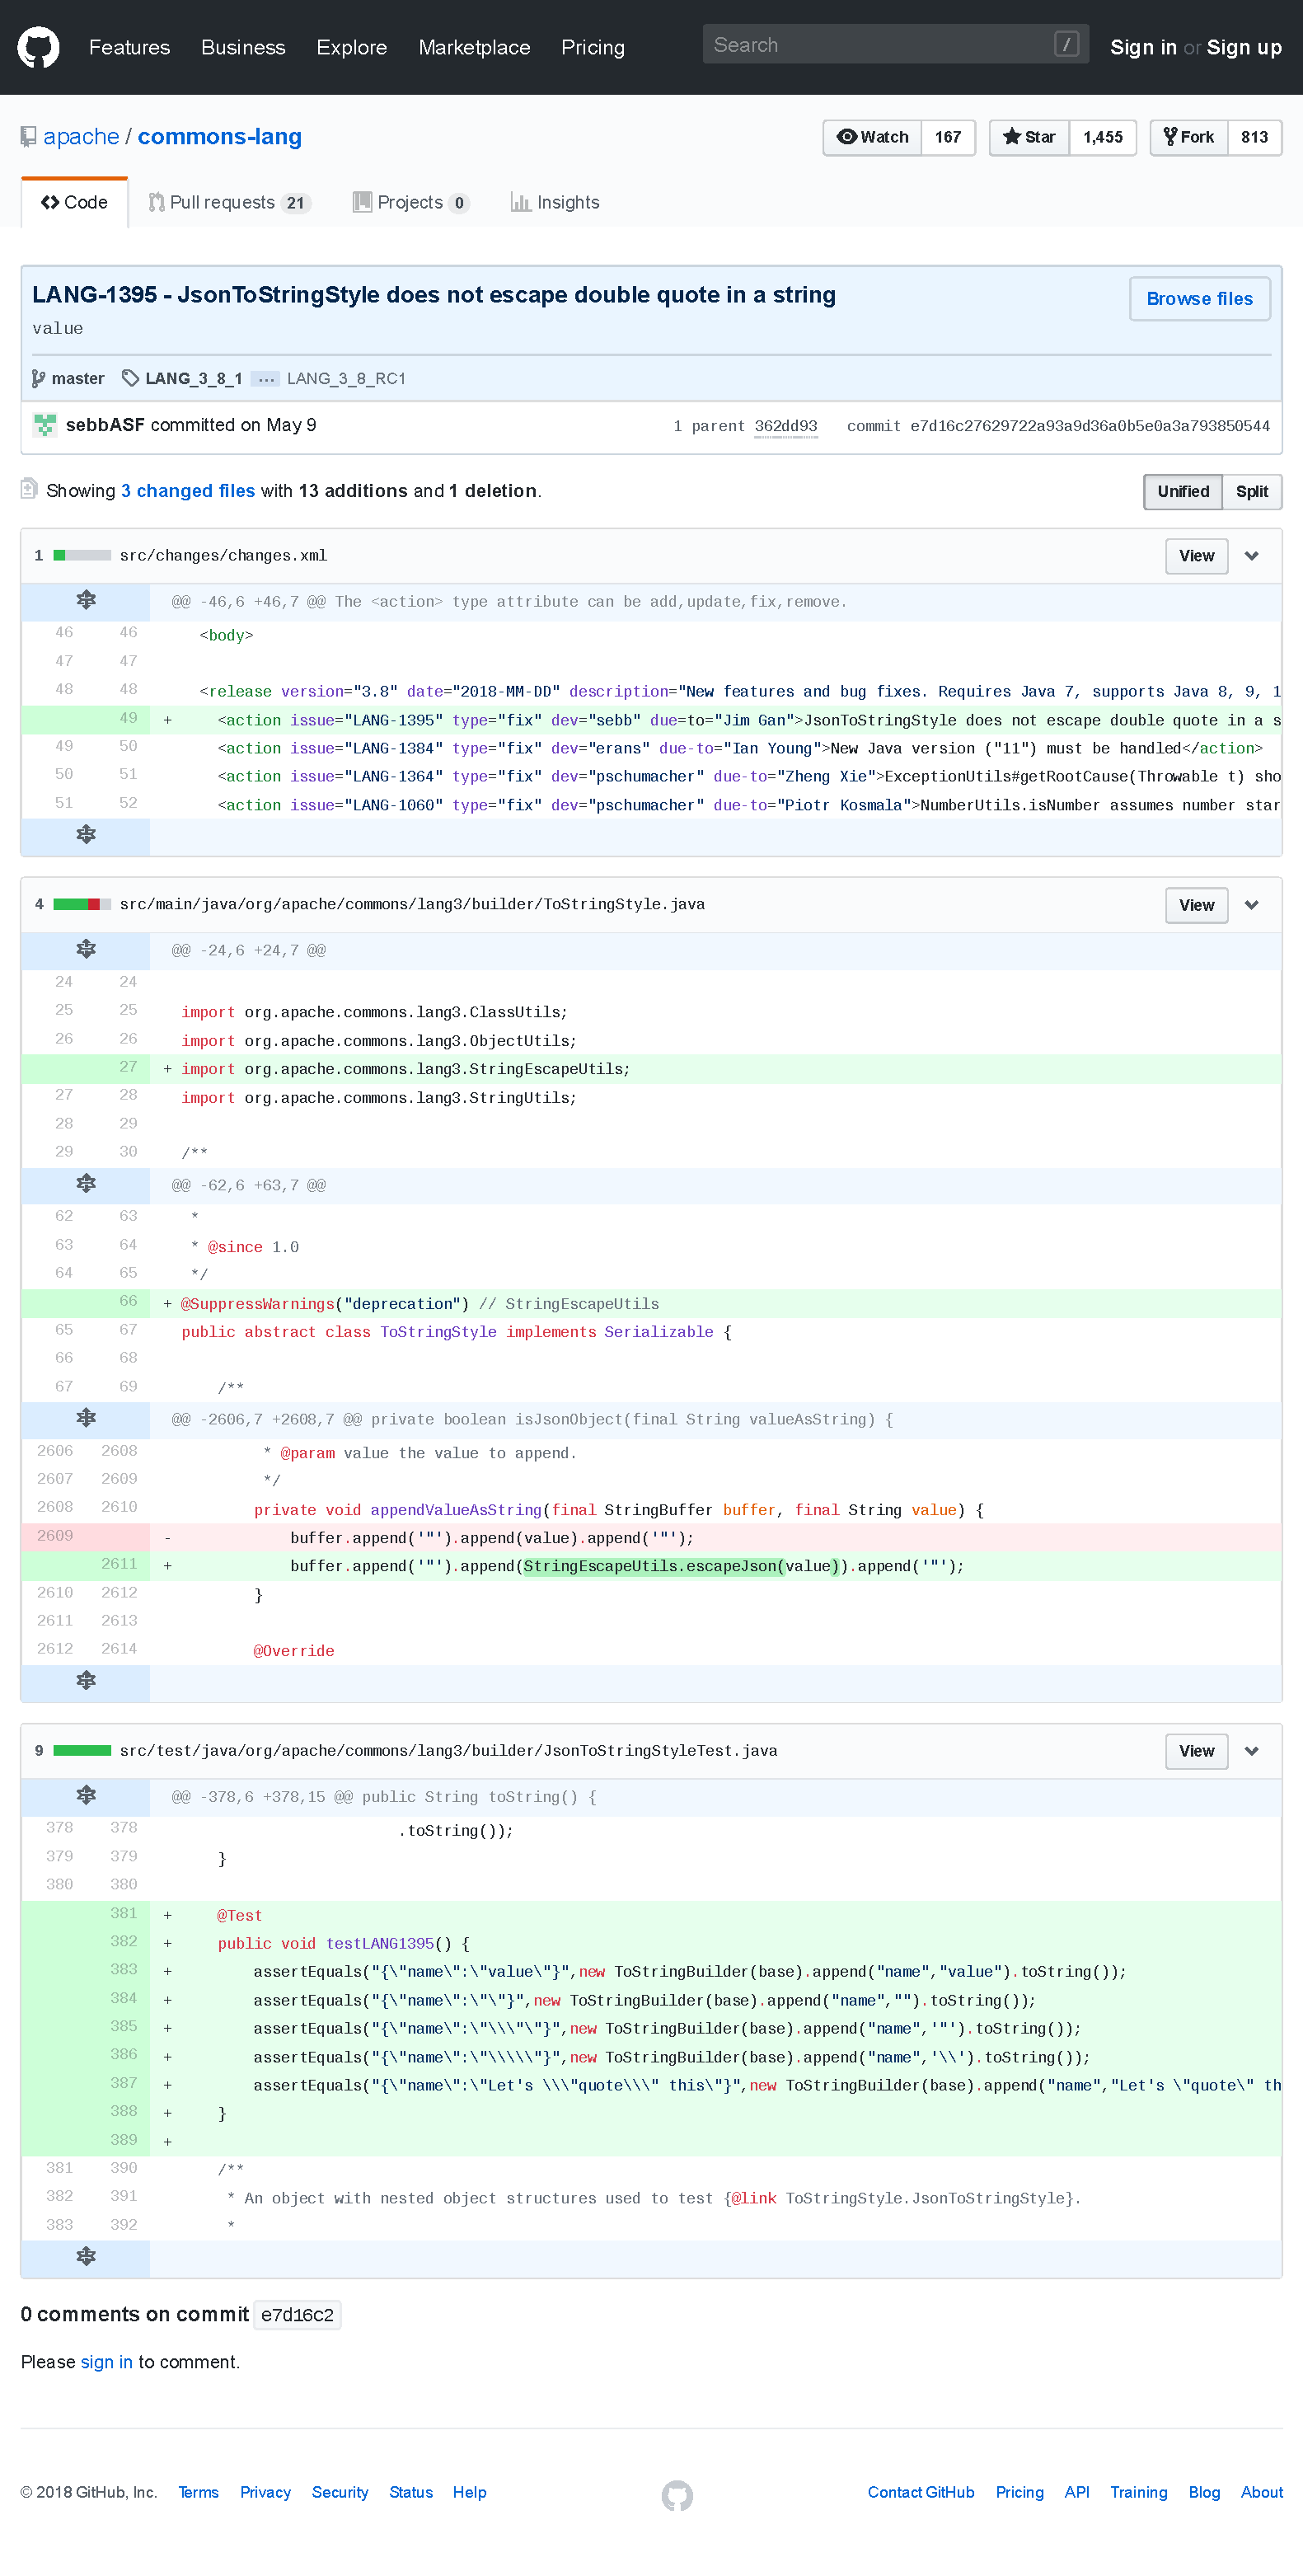
\includegraphics[width=.97\linewidth, trim=4.5cm 9.2cm 5.8cm 39.2cm, clip]{img/diff/diff-commons-lang.pdf}}
\caption{Developer test for \textsc{e7d16c2} of commons-lang.}
\label{fig:diff_commons-lang}
\end{figure}


%% GSON
\textsc{gson\#44cad04}\footnote{\url{https://github.com/google/gson/commit/44cad04}}: This commit allows Gson to deserialize a number represented as a string.
\autoref{fig:ampl_gson} shows the relevant part of the test generated by DCI$_{SBAMPL}$, based on \texttt{testNumberDeserialization} of \texttt{PrimitiveTest} as a seed.
First, we see that the test selected as a seed is indeed related to the change in the deserialization feature.
The DCI test detects the behavioral change at lines 3 and 4.
On the pre-commit version, line 3 throws a \texttt{JsonSyntaxException}.
On the post-commit version, line 4 throws a \texttt{NumberFormatException}.
In other words, the behavioral change is detected by a different exception (different type and not thrown at the same line).
\footnote{Interestingly, the number is parsed lazily, only when needed. Consequently, the exception is thrown when invoking the \texttt{longValue()} method and not when invoking \texttt{parse()}}.

\begin{figure}[h]
\centering
\fbox{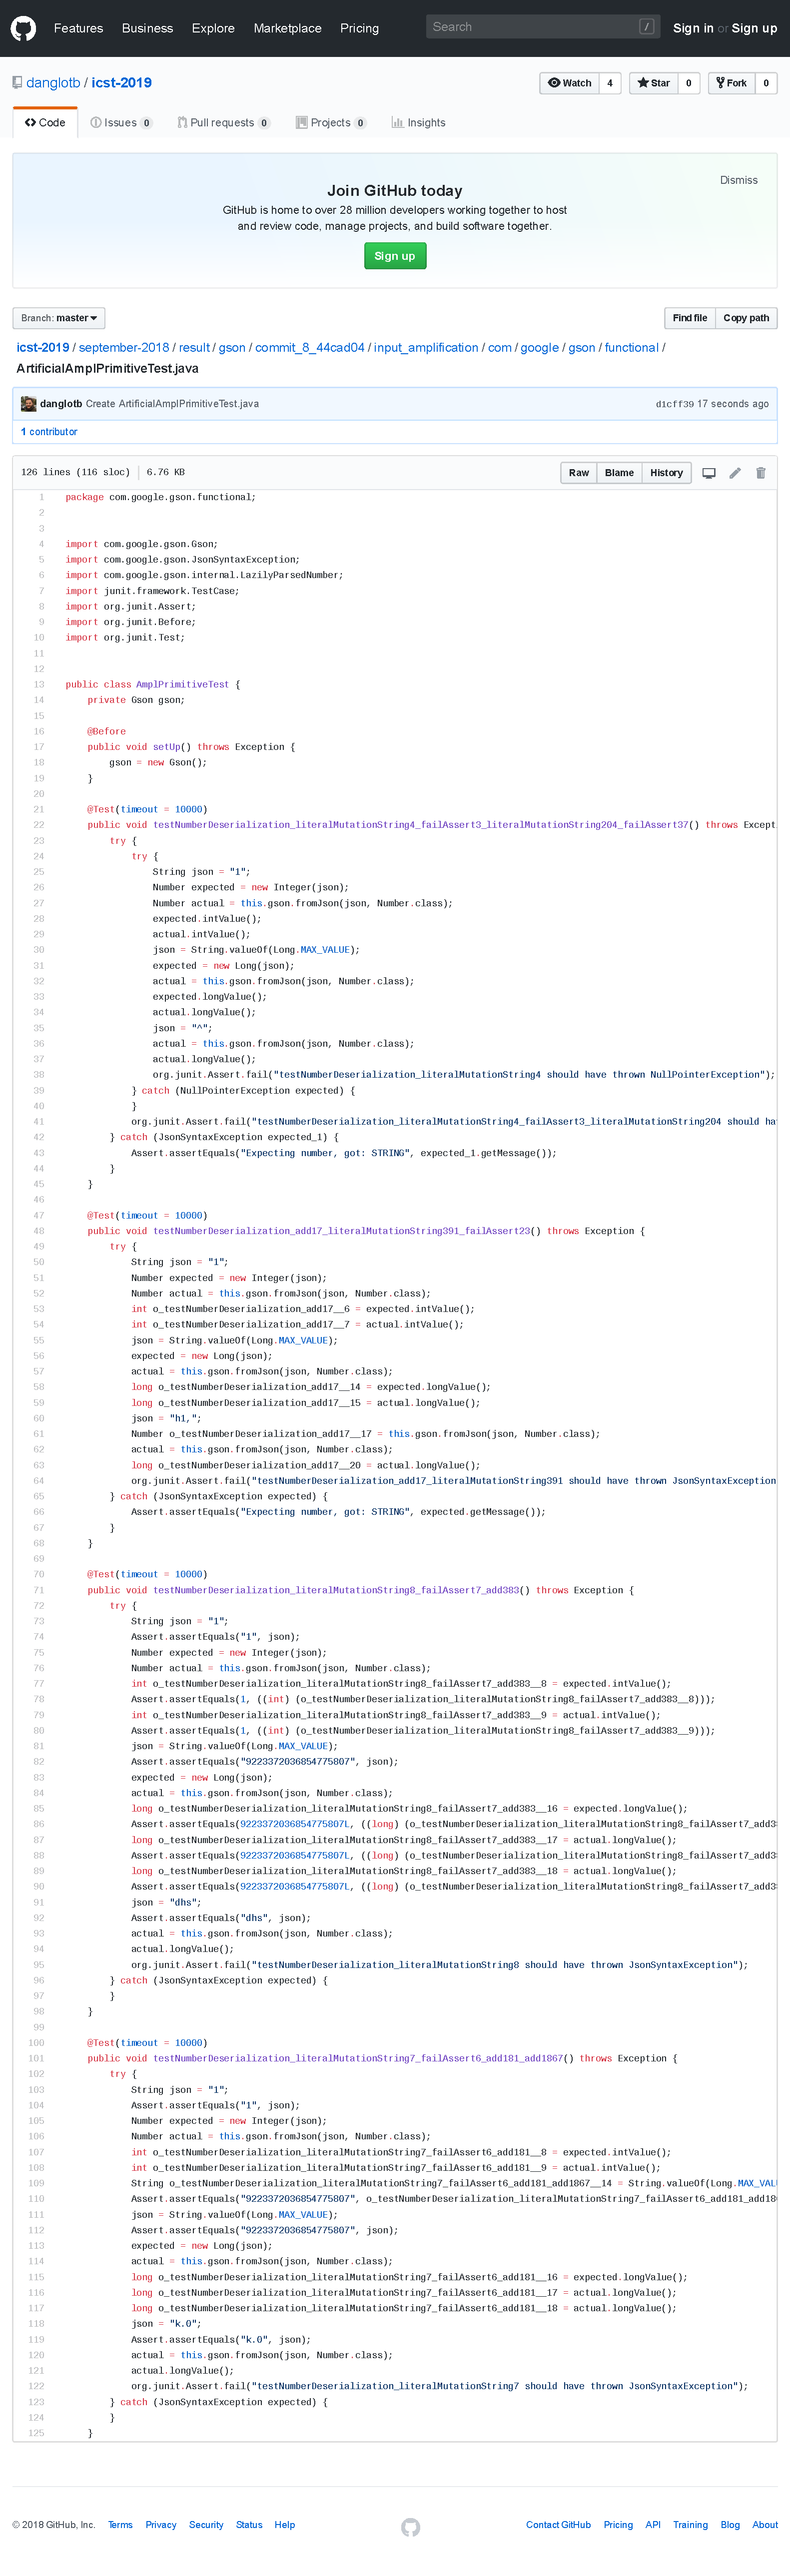
\includegraphics[width=.95\linewidth, trim=3.7cm 19.5cm 13.4cm 64.2cm, clip]{img/amplified/ampl-gson.pdf}}
\caption{Test generated by DCI that detects the behavioral change of commit \textsc{44cad04} in Gson.}
\label{fig:ampl_gson}
\end{figure}

We compare it against the developer-written ground-truth method, shown in \autoref{fig:diff_gson}. 
This short test verifies that the program handles a number-as-string correctly.
For this example, the DCI test does indeed detect the behavioral change, but in an indirect way.
On the contrary, the developer test is shorter and directly targets the changed behavior, which is better.

\begin{figure}[h]
\centering
\fbox{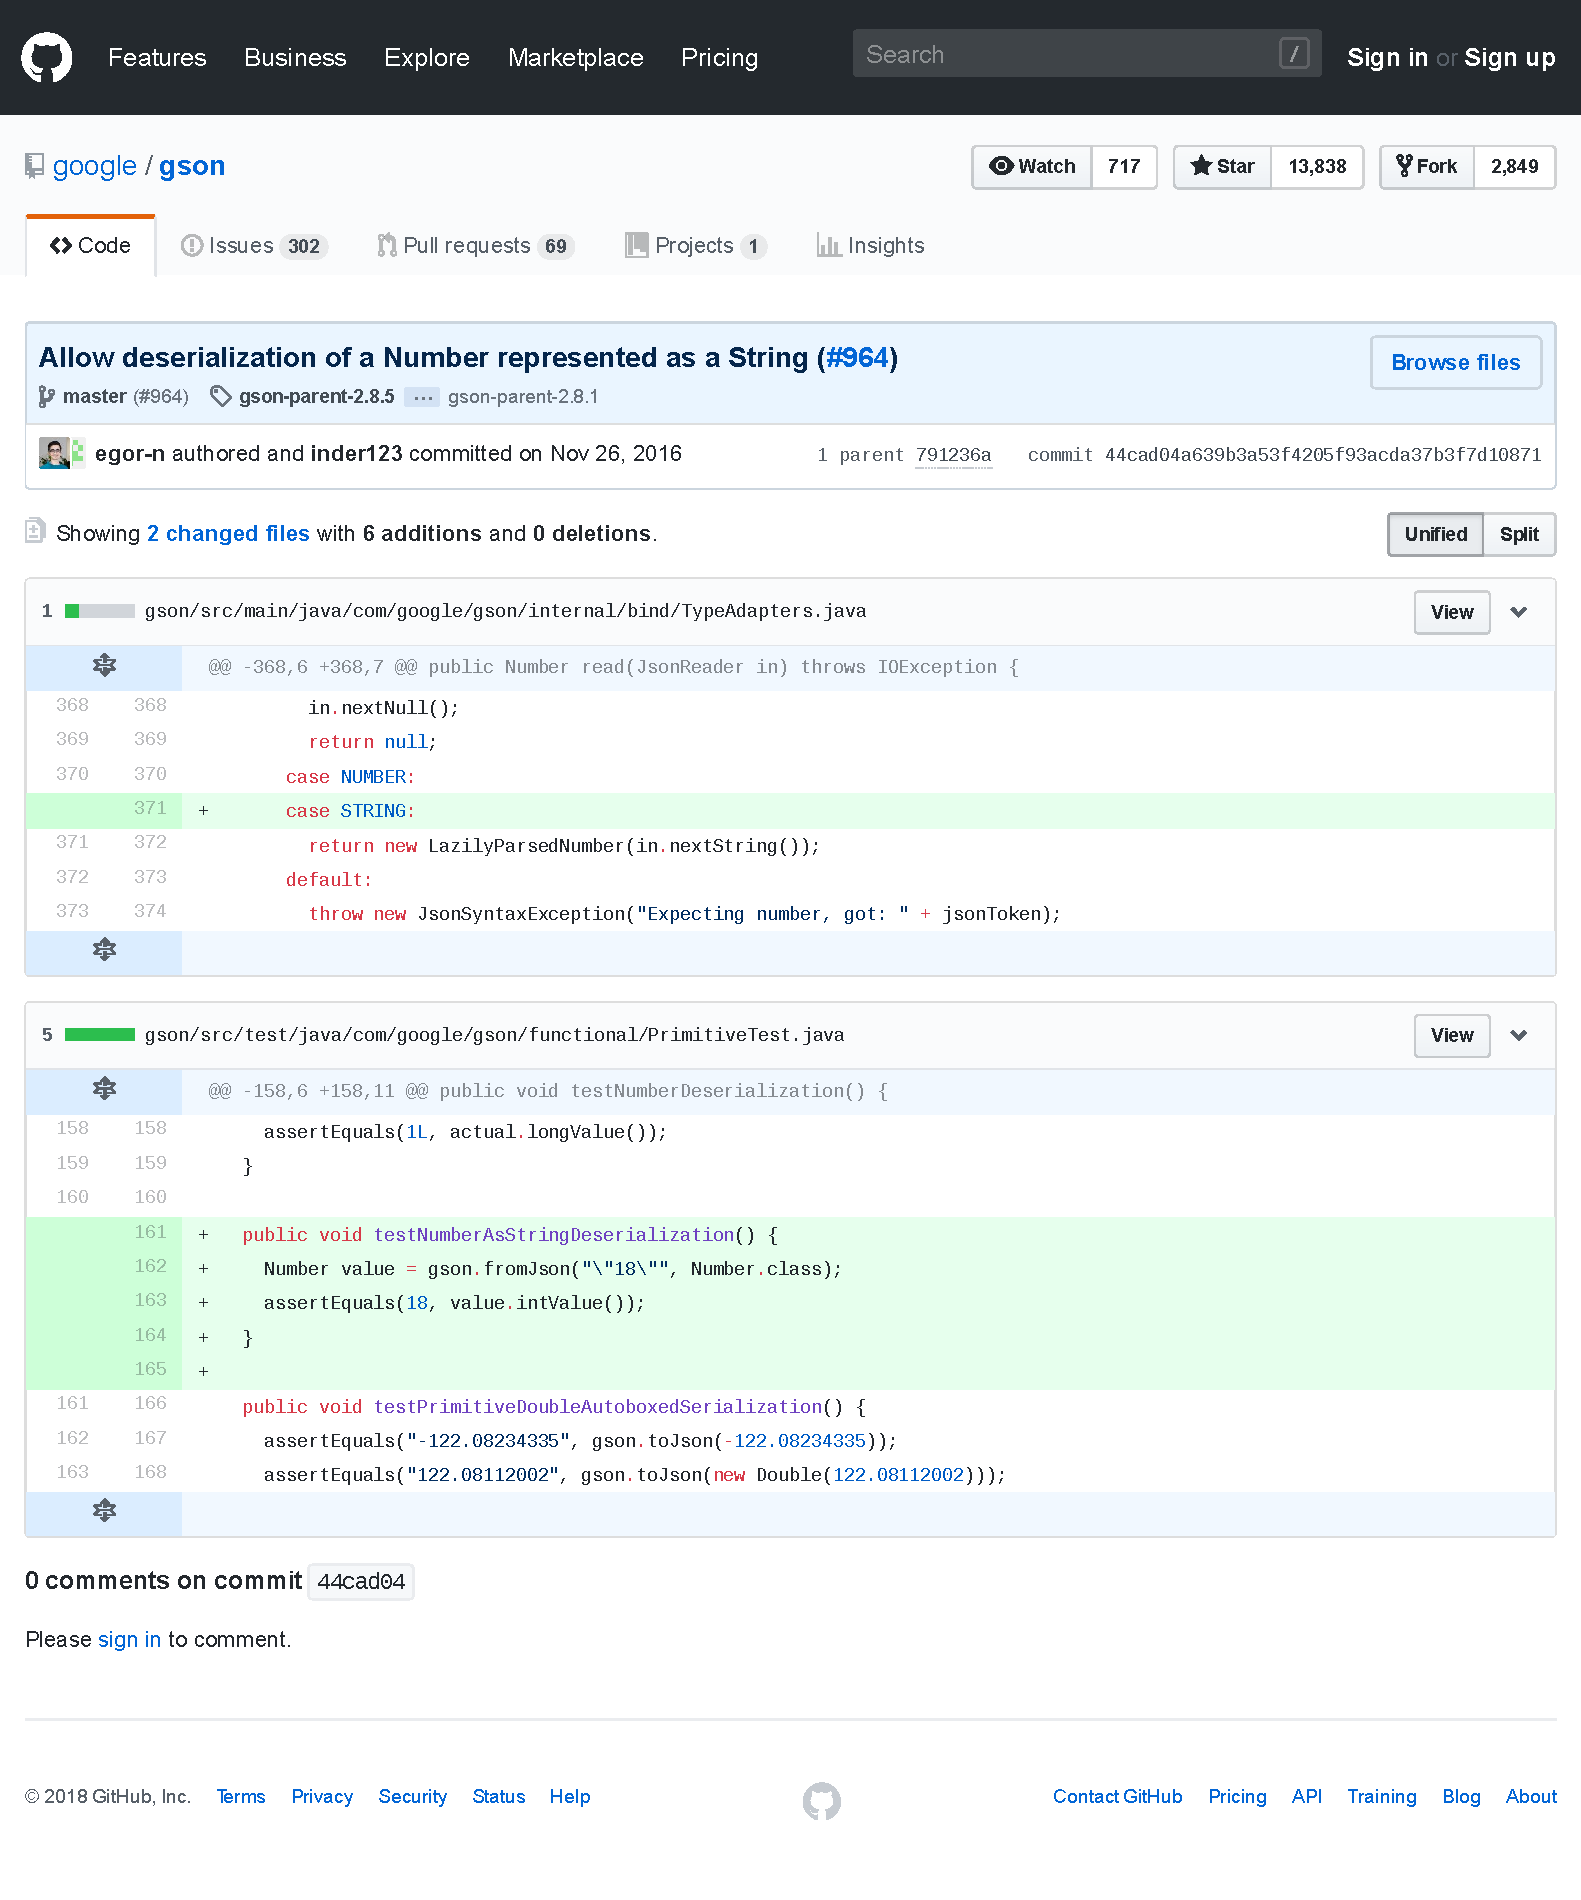
\includegraphics[width=.95\linewidth, trim=4cm 9.3cm 12.5cm 20.6cm ,clip]{img/diff/diff-gson.pdf}}
\caption{Provided test by the developer for \textsc{44cad04} of Gson.}
\label{fig:diff_gson}
\end{figure}



%% JSOUP
\textsc{jsoup\#3676b13}\footnote{\url{https://github.com/jhy/jsoup/commit/3676b13}}: This change is a pull request (\ie a set of commits) and introduces 5 new behavioral changes. There are two improvements: skip the first new lines in pre tags and support deflate encoding, and three bug fixes: throw exception when parsing some urls, add spacing when output text, and no collapsing of attribute with empty values.
\autoref{fig:ampl_jsoup} shows an amplified test obtained using \DCII.
This amplified test has 15 assertions and a duplication of method call.
Thanks to this duplication and assertion generated on the \texttt{toString()} method, this test is able to capture the behavioral change introduced by the commit.

\begin{figure}[h]
\centering
\fbox{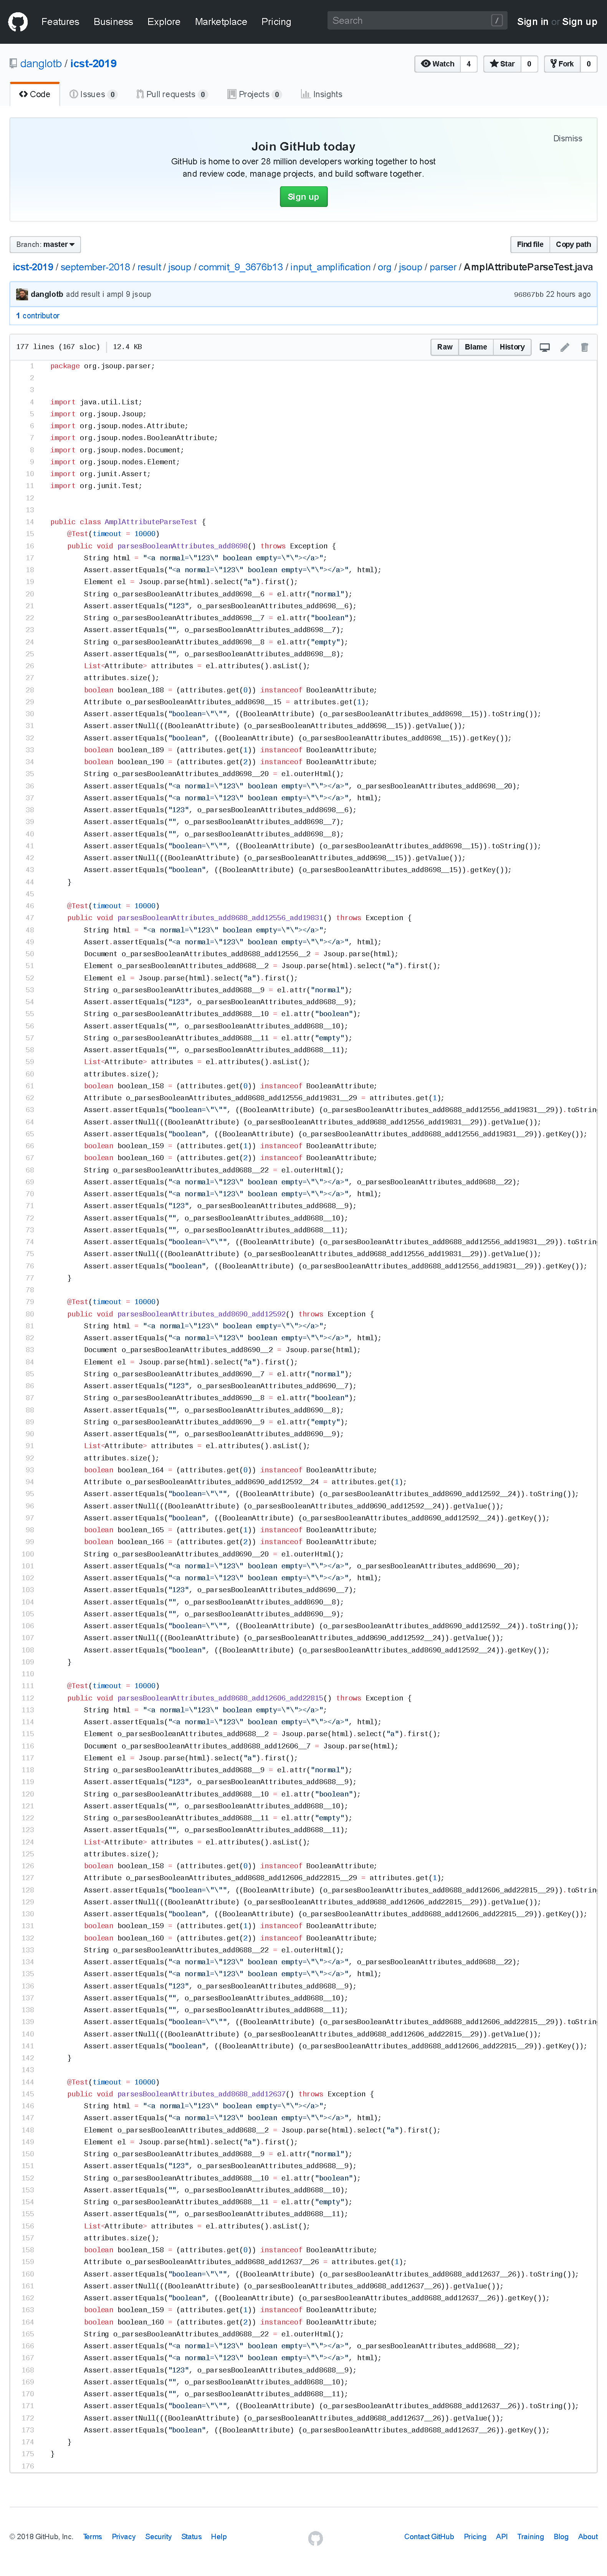
\includegraphics[width=.95\linewidth, trim=3.7cm 82cm 7cm 30.8cm ,clip]{img/amplified/ampl-jsoup.pdf}}
\caption{Test generated by \DCII that detects the behavioral change of \textsc{3676b13} of Jsoup.}
\label{fig:ampl_jsoup}
\end{figure}

As before, we compare it to the developer's test. 
The developer uses the \texttt{Element} and \texttt{outerHtml()} methods rather than \texttt{Attribute} and \texttt{toString()}.
However, the method \texttt{outerHtml()} in \texttt{Element} will call the \texttt{toString()} method of \texttt{Attribute}.
For this behavioral change, it concerns the \texttt{Attribute} and not the \texttt{Element}.
So, the amplified test is arguably better, since it is closer to the change than the developer's test.
But, \DCII generates amplified tests that detect 2 of 5 behavioral changes: adding spacing when output text and no collapsing of attribute with empty values only, so regarding the quantity of changes, the human tests are more complete.

\begin{figure}[h]
\centering
\fbox{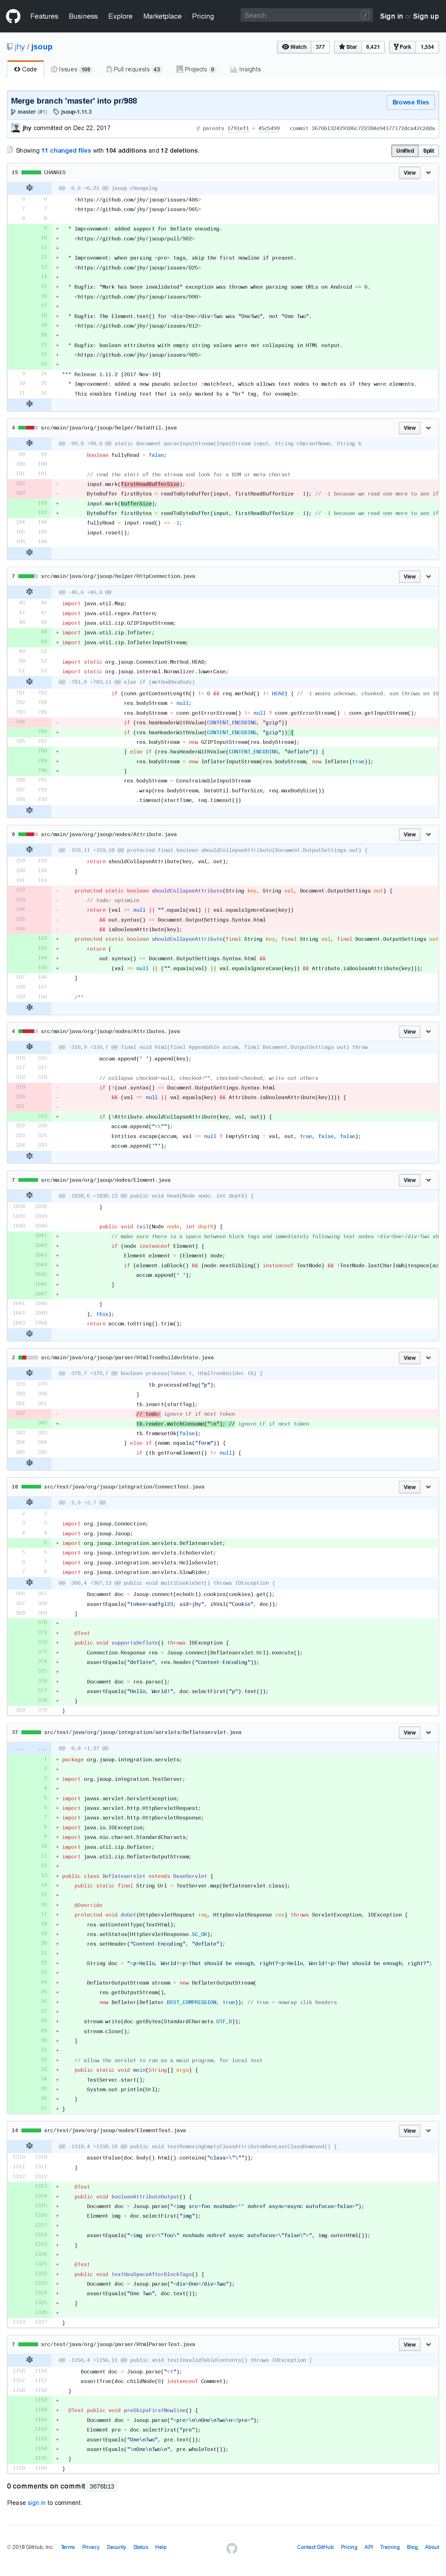
\includegraphics[width=.95\linewidth, trim=4.3cm 19.6cm 4.8cm 131.5cm , clip]{img/diff/diff-jsoup.pdf}}
\caption{Provided test by the developer for \textsc{3676b13} of Jsoup.}
\label{fig:diff_jsoup}
\end{figure}

%%%%%%%%%%%%%%%%%%%%%%%%%%%%%%%%%%%%%%%
%% MUSTACHE JAVA
\textsc{Mustache.java\#774ae7a}\footnote{\url{https://github.com/spullara/mustache.java/commit/774ae7a}}: This commit fixes an issue with the usage of a dot in a  relative path on Window in the method \texttt{getReader} of class \texttt{ClasspathResolver}.
The test method \texttt{getReaderNullRootDoesNotFindFileWithAbsolutePath} has been used as seed by DCI. It modifies the existing string literal with another string used somewhere else in the test class and generates 3 new assertions.
The behavioral change is detected thanks to the modified strings: it produces the right test case containing a space.

\begin{figure}[h]
\centering
\fbox{
\includegraphics[width=.95\linewidth]{img/amplified/ampl-mustache.png}}
\caption{Test generated by \DCII that detects the behavioral change of \textsc{774ae7a} of Mustache.java.}
\label{fig:ampl_mustache}
\end{figure}

The developer proposed two tests that verify that the object reader is not null when getting it with dots in the path.
There are shown in \autoref{fig:diff_mustache}.
These tests invoke the method \texttt{getReader} which is the modified method in the commit.
%
The difference is that the \DCII's amplified test method provides a non longer valid input for the method \texttt{getReader}.
However, providing such inputs produce errors afterward which signal the behavioral change.
In this case, the amplified test is complementary to the human test since it verifies that the wrong inputs are no longer supported and that the system immediately throws an error.

\begin{figure}[h]
\centering
\fbox{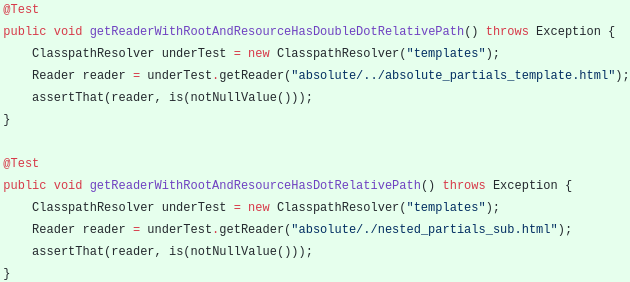
\includegraphics[width=.95\linewidth]{img/diff/diff-mustache.png}}
\caption{Developer test for \textsc{774ae7a} of Mustache.java.}
\label{fig:diff_mustache}
\end{figure}

%%%%%%%%%%%%%%%%%%%%%%%%%%%%%%%%%%%%%%%
%% XWIKI COMMONS
\textsc{xwiki-commons\#d3101ae}\footnote{\url{https://github.com/xwiki/xwiki-commons/commit/d3101ae}}: This commit fixes a bug in the \texttt{merge} method of class \texttt{DefaultDiffManager}.
\autoref{fig:ampl_xwiki} shows the amplified test method obtained by \DCIA.
DCI used \texttt{testMergeCharList} as a seed for the amplification process, and generates 549 new assertions.
Among them, 1 assertion captures the behavioral change between the two versions of the program: 
``assertEquals(0, result.getLog().getLogs(LogLevel.ERROR).size());''.
The behavioral change that is detected is the presence of a new logging statement in the diff. After verification, there is indeed such a behavioral change in the diff, with the addition of a call to ``logConflict'' in the newly handled case.

\begin{figure}[h]
\centering
\fbox{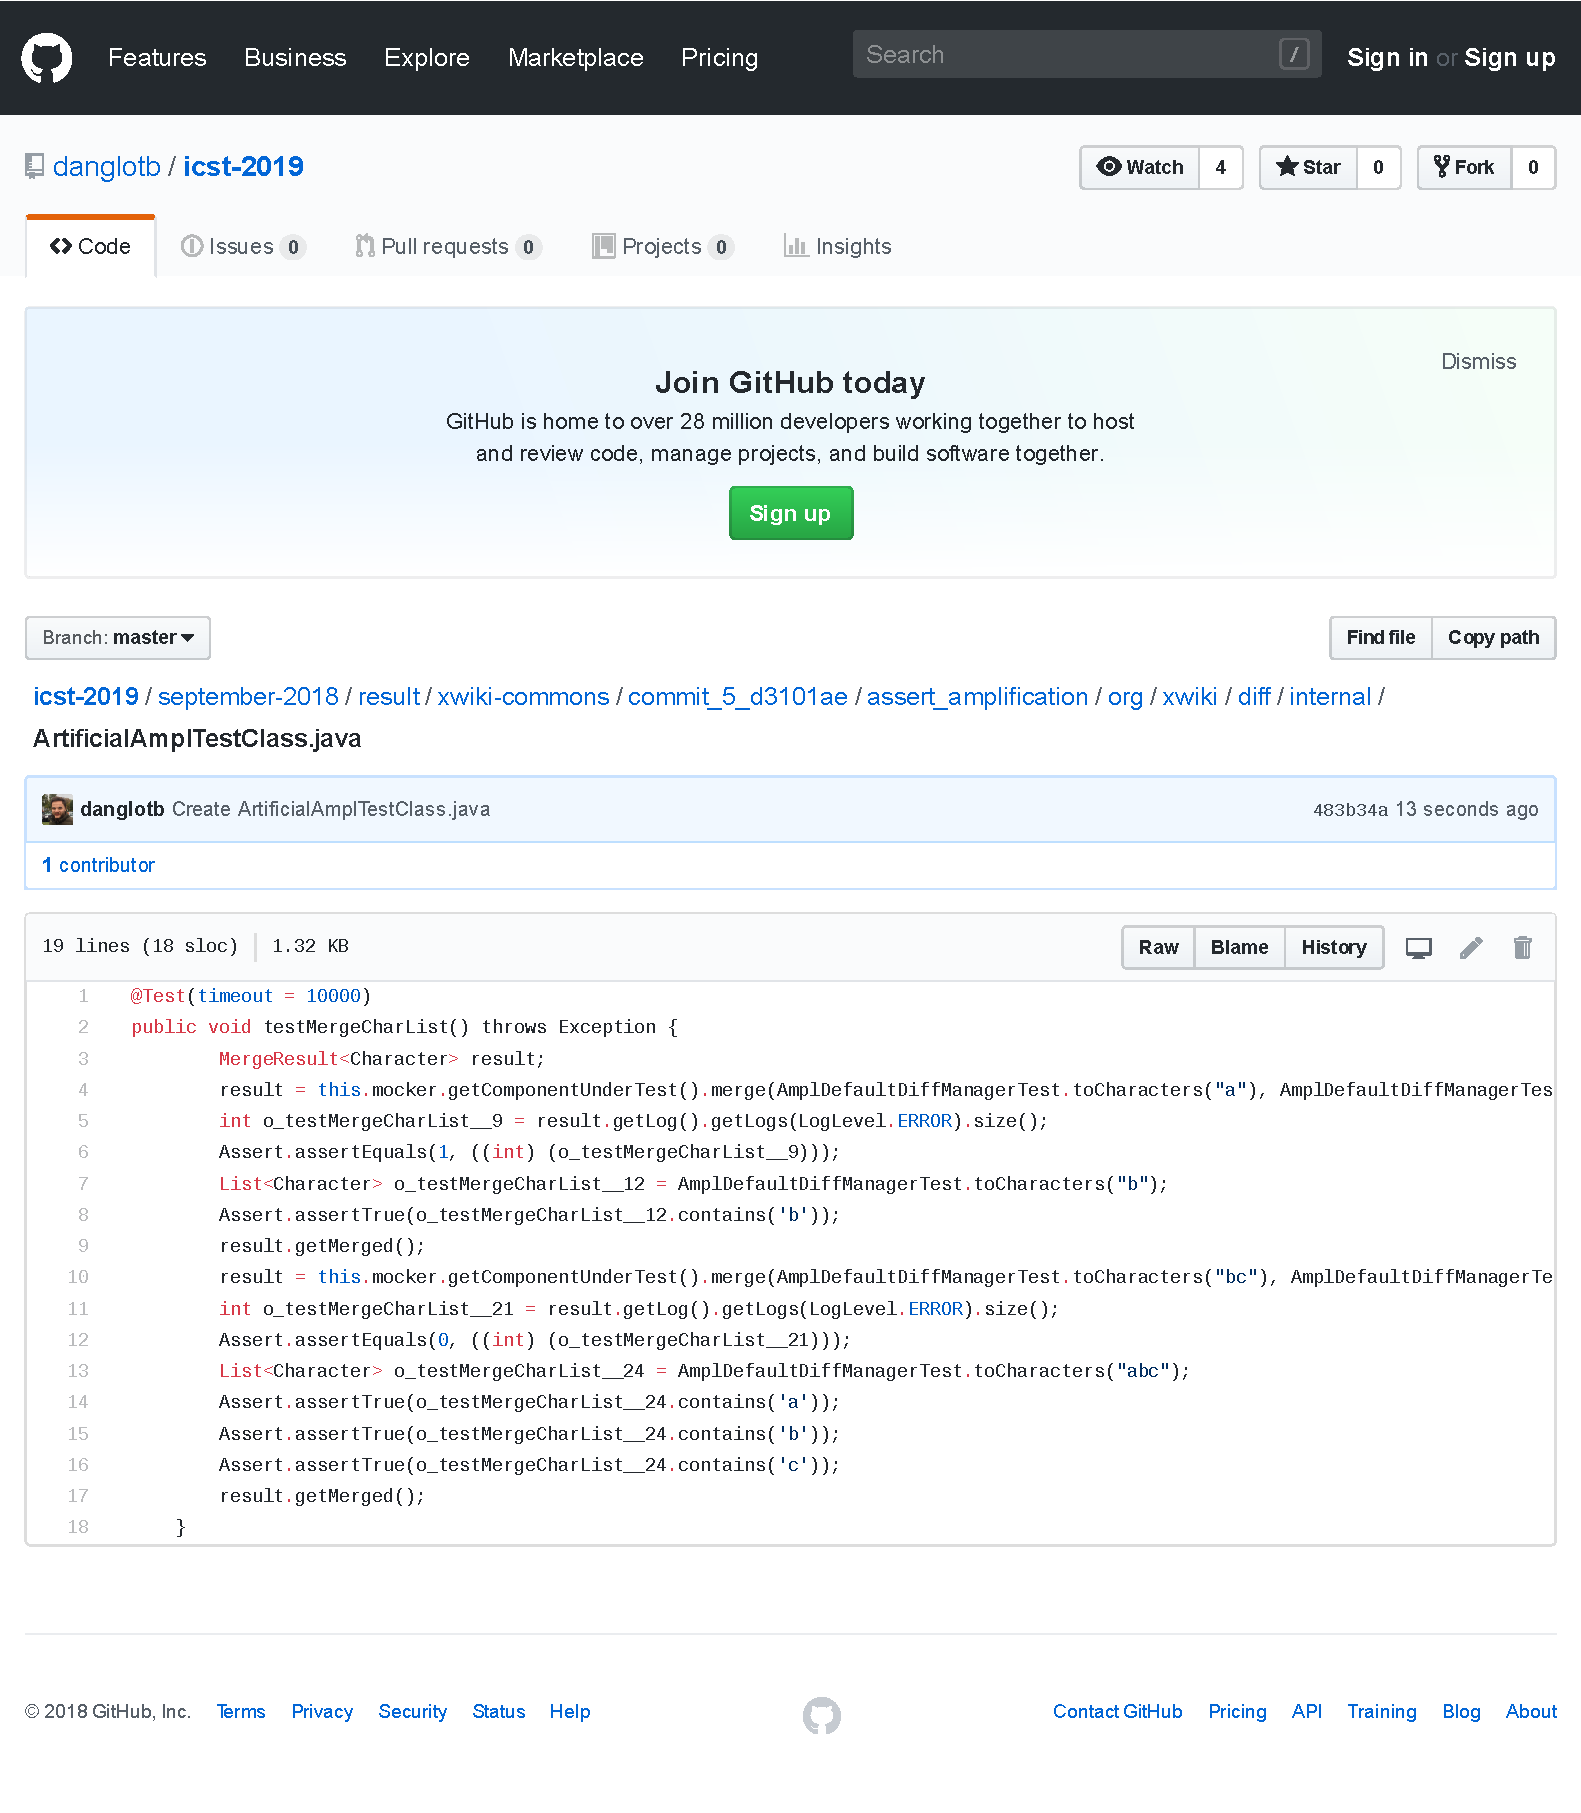
\includegraphics[width=.95\linewidth, trim=3.5cm 11.5cm 9.2cm 18.2cm, clip ]{img/amplified/ampl-xwiki.pdf}}
\caption{Test generated by \DCIA that detects the behavioral change of \textsc{d3101ae} of XWiki.}
\label{fig:ampl_xwiki}
\end{figure}

The developer's test is shown in \autoref{fig:diff_xwiki}.
This test method directly calls method \texttt{merge}, which is the method that has been changed. 
What is striking in this test is the level of clarity: the variable names, the explanatory comments and even the vertical space formatting are impossible to achieve with \DCIA and makes the human test clearly of better quality but also longer to write. % above when she has the time to write a good test. 
%
Yet, \DCIA's amplified tests capture a behavioral change that was not specified in the human test.
In this case, amplified tests can be complementary.

\begin{figure}[h]
\centering
\fbox{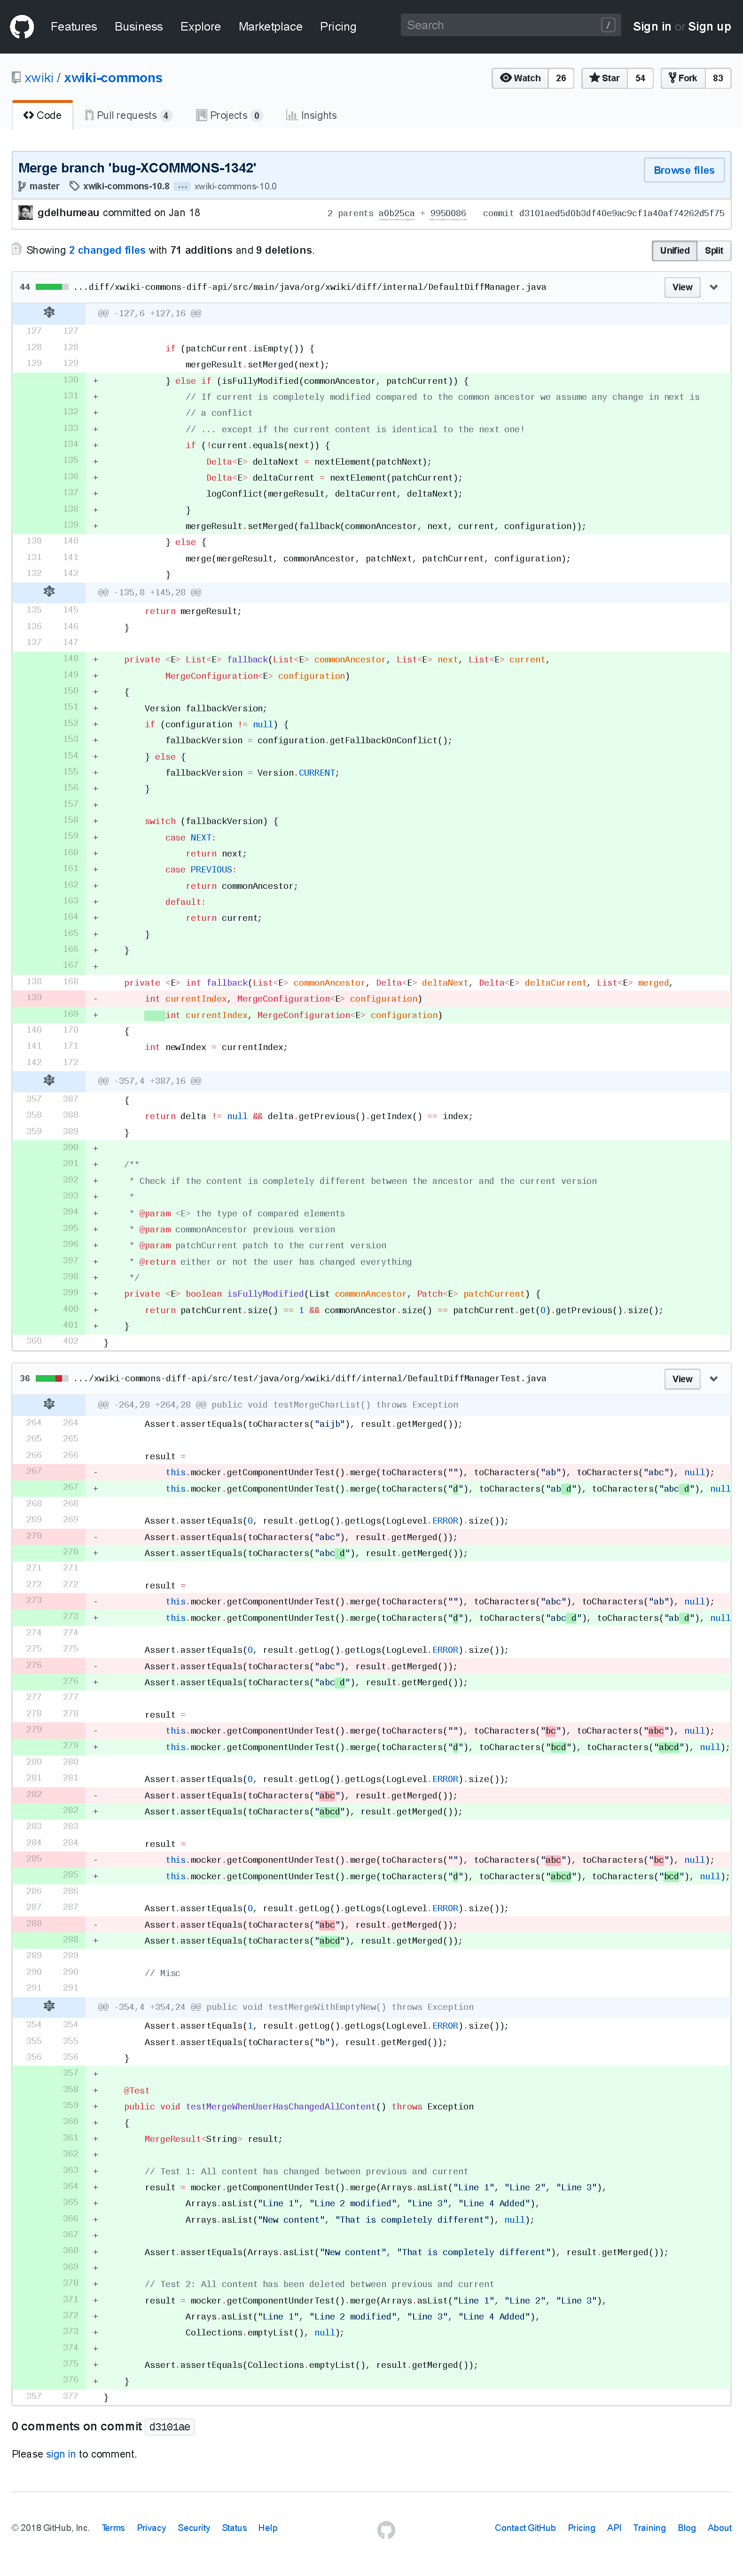
\includegraphics[width=.95\linewidth, trim=4.2cm 6.7cm 5cm 75cm, clip]{img/diff/diff-xwiki.pdf}}
\caption{Developer test for \textsc{d3101ae} of XWiki.}
\label{fig:diff_xwiki}
\end{figure}


\begin{mdframed}
Answer to \textbf{RQ4}: 
In 2 of 5 cases, the DCI test is complementary to the human test.
In 1 case, the DCI test can be considered better than the human test.
In 2 cases, the human test is better than the DCI test.
Even though human tests can be better, DCI can be complementary and catch missed cases, or can provide added-value when developers do not have the time to add a test.
\end{mdframed}

%\pagebreak


% -----------------------
%  Main Observed Limitation
% -----------------------
\section{Discussion about the scope of DCI}
\label{sec:limitation}

In this section, we overview the current limitations of DCI and the key factors that prevent DCI from amplifying test methods that detect behavioral changes.

\textbf{Time consumption}
From our experiments, we see that the time consumption to complete the amplification is the main limitation of DCI.
\textsc{jsoup\#2c4e79b}, almost 5 hours have been spent with no result.
For the sake of our experimentation, we choose to use a pre-defined number of iteration to bound the exploration.
In practice, we recommend to set a time budget (\eg at most one hour per pull-request).

\textbf{Importance of test seeds}
By construction, DCI's effectiveness is correlated to the test methods used as seed.
For example, see the row of \texttt{commons-lang\#c8e61af} in \autoref{tab:overall_result_iteration}
where one can observe that whatever the number of iteration, DCI takes the same time to complete the amplification.
The reason is that the seed tests are only composed of assertions statements.
Such tests are bad seeds for DCI and they prevent any good input amplification.

\textbf{False positive}
The risk of false positives is a potential  limitation of your approach.
A false positive would be an amplified test method that passes or fails on both versions, which means that the amplified test method does not detect the behavioral difference between both versions.
We manually  analyzed 6 commits and none of them are false positives.
While this is not a proof that DCI would never produce such confusing test methods, we are confident in the soundness of our implementation.

% -----------------------
%  THREATS
% -----------------------
\section{Threats to validity}
\label{sec:threats}

% bug in the implementation
An internal threat is the potential bugs in the implementation of DCI. However, we heavily tested our prototype with JUnit test cases to mitigate this threat.

% benchmark
In our benchmark, there are 60 commits. Our result may be not be generalizable to all programs. But we carefully selected real and diverse applications from GitHub, all having a strong test suite. We believe that the benchmark reflects real programs, and we have good confidence in the results.

% flaky amplified test
Last but not least threat is the potential flakiness of generated test methods.
However we take care that our approach does not produce flaky test methods, and we make sure to observe a stable and different state of the program between different executions. 
To do this, we execute 3 times each amplified test in order to check weather or not there are stable.
If the outcome of a at least one execution is different than the others, we discard the amplified test.

% weak statiscal test
For the evaluation of the randomness, we use a Kruskal-Willis, which is known to be weaker than ANOVA test.
To perform an ANOVA test, the data must fulfull the following criteria:
1) The samples are independent;
2) Each sample is from a normally distributed population;
3) The population standard deviations of the groups are all equal. This property is known as homoscedasticity.
The two first are fulfilled while the third is not:
\begin{table*}
\def\arraystretch{1}%  1 is the default, change whatever you need
\setlength\tabcolsep{3pt} % default value: 6pt
\caption{Standard deviations of the number of amplified tests obtained for each seed.}
\begin{tabular}{c|cccccccccc}
seed     & 1 & 2 & 3 & 4 & 5 & 6 & 7 & 8 & 9 & 10 \\
\hline
std     & 63.38&63.55&62.56&61.27&61.33&61.66&63.76&60.91&61.25&63.35
\end{tabular}
\end{table*}
Since the standard deviations are not all equal, the associated p-value would not be valid.
This is why we choose to use a Kruskal-Willis test.

In addition to this, we perform it for only 11 seeds, which a small samples.

% -----------------------
%  RELATED - WORK
% -----------------------
\section{Related Work}
\label{sec:related_work}

\subsection{Commit-based test generation}

Person \etal~\cite{dse} present differential symbolic execution (DSE). DSE combines symbolic execution and a new approximation technique to highlight behavioral changes.
They use symbolic execution summary to find equivalences and difference and generate a set of inputs that trigger different behavior.
This is done in three steps: 1) they execute both versions of the modified method; 2) they find equivalences and differences, thanks to the analysis of symbolic execution summary;  3) they generate a set of inputs that trigger the different behaviors in both versions.
The main difference with our work is that they have the strong assumption to have a program whose semantics is fully handled by the symbolic execution engine. 
In the context of Java, to our knowledge, no symbolic execution engine works on arbitrary Java program.
Symbolic execution engines do not scale to the size and complexity of the programs we targeted.
On the contrary, our approach, being more lightweight, is meant to work on all Java programs.

Marinescu and Cadar~\cite{marinescu2013katch} present Katch, a system that aims at covering the code included in a patch.
This approach first determines the differences of a program and its previous version.
It targets modified and not executed by the existing test suite lines.
Then, it selects the closest input to each target from existing tests using a static minimum distance over the control flow graph.
The proposal is evaluated on Unix tools. 
They examine patches from a period of 3 years. In average, they automatically increase coverage from 35\% to 52\% with respect to the manually written test suite.
Contrary to our work, they only aim at increasing the coverage, not at detecting behavioral changes.

A posterior work of the same group~\cite{palikareva2016shadow,Kuchta:2018:SSE:3276753.3208952} focuses on finding test inputs that execute different behaviors in two program versions. 
They devise a technique, named ShaddowKlee, built on top of Klee \cite{klee}. 
They require the code to be annotated at changed places. 
Then they select from the test suite those test cases that cover the changed code. The unified program is used in a two stage dynamic symbolic execution guided by the selected test cases.
They first look for branch points where the conditions are evaluated in both program versions.
Then, a constraint solver generates new test inputs for divergent scenarios. The program versions are then normally executed with the generated inputs and the result is validated to check the presence of a bug or of an intended difference.
The evaluation of the proposed method is based on the CoREBench~\cite{bohme2014corebench} data set that contains documented regression bugs of the GNU Coreutils program suite. 


Noller \etal~\cite{jpfshadow} aim at detecting regression bugs. 
They apply shadow symbolic execution, originally from Palikevera~\cite{dse,palikareva2016shadow} that has been discussed in the previous paragraph, on Java programs. 
Their approach has been implemented as an extension of Java Path Finder Symbolic (jpf-symbc)\cite{jpfsymb}, named jpf-shadow. 
Shadow symbolic execution generate test inputs that trigger the new program behavior. 
They use a merged version of both version of the same program, i.e. the previous version, so called old, and the changed version, called new.
This is done by instrumenting the code with method calls ``change()''.
The method change() takes two inputs: the old statement and the new one.
Then, a first step collects divergence points, i.e. conditional where the old version and the new version do not take the same branch.
On small examples, they show that jpf-shadow generates less unit test cases yet cover the same number of path. 
Jpf-shadow only aims at covering the changes and not at detecting the behavioral change with an assertion.

Menarini \etal~\cite{semantics:code:review} proposes a tool, GETTY, based on invariants mined by Daikon.
GETTY provides to code reviewers a summary of the behavioral changes, based on the difference of invariants for various combinations of programs and test suites.
They evaluate GETTY on 6 open source project, and showed that their behavioral change summaries can detect bugs earlier than with normal code review.
While they provide a summary, DCI provides a concrete test method with assertions that detect the behavioral changes. 

Lahiri \etal~\cite{differential-assertion-checking} propose differential assertion checking (DAC): checking two versions of a program with respect to a set of assertions. DAC is based on filtering false alarms of verification analysis. They evaluate DAC on a set of small example.
The main difference is that DAC requires to manually write specifications, while DCI is completely automated with normal code as input.

Yang \etal~\cite{Yang:2014:PDI:2568225.2568319} introduce IProperty, a  way to annotate  correctness properties of programs. They evaluate their approach on the triangle problem.
The key novelty of our work is to perform an evaluation on real commits from large scale open source software.

Campos \etal~\cite{Campos:2014:CTG:2642937.2643002} extended EvoSuite to adapt test generation techniques to continuous integration.
Their contribution is the design of a time budget allocation strategy: it allocates more time budget to specific classes that are involved in the changes.
They evaluated their approach on 10 projects from the SF100 corpus, on 8 of the most popular open-source projects from GitHub, and on 5 industrial projects.
They limit their evaluation to the 100 last consecutive commits.
They observe an increase of +58\% branch coverage, +69\% thrown undeclared exceptions, while reducing the time consumption by up to 83\% compared to the baseline.
The major difference compared to our approach, they do not aim at specifically obtaining test methods that detect the behavioral changes but rather obtain better branch coverage and detect undeclared exceptions. They also do not generate any assertions.
However, from the point of view practitioners, integrating a time budget strategy into DCI would increase its usability, practicability and potential adoption.


\subsection{Behavioral change detection}

Evans \etal \cite{evans2007differential} devise the differential testing.
This approach aims at alleviating the test repair problem and detects more changes than regression testing alone.
They use an automated characterization test generator (ACTG) to generate test suite for both version of the program.
They then categorizes the tests of these 2 test suites into 3 groups:
1) $T_{preserved}$ which are the tests that pass on the both versions;
2) $T_{regressed}$ which are the tests that pass on the previous version but not on the new one;
3) $T_{progressed}$ which are the tests that pass on the new version but not on the previous one;
Then, they define also $T_{different}$ which is the union of both $T_{regressed}$ and $T_{progressed}$.
The approach is to execute $T_{different}$ on both versions and observe progressed and regressed behaviors.
They evaluate their approach on a small use case from the SIR dataset on 38 diffrent changes, for version of the program.
They showed that their approach detects 21\%, 34\%, and 21\% more behavior changes than regression testing alone for respectively version 1, version 2 and version 3.
In DCI, the amplified test methods obtained would lie into the $T_{regressed}$ group.
However, we could also amplified test methods using the new version of the program and obtain a $T_{progressed}$.
We would obtain a $T_{different}$ of amplified test methods and it might improve the performance of DCI.
About the evaluation, we run experimentation of 60 commits which the double than their dataset, and on real 
projects and real commits from \gh.

Wei Jin \etal \cite{automated-behavioral-regression-testing} propose BEhavioral Regression
Testing BERT.
BERT aims at assisting practitioners during development to identify potential regression.
It has been implemented as a plugin for the IDE Eclipse.
Each time a developer make a change in their code base and Eclipse compiles, BERT is triggered.
BERT works in 3 phases:
1) it analyzes what are the classes modified and runs a test generation tools, such as Randoop, to create new test input for these classes.
2) it executes the generated tests on both version of the program and collect multiples values such as the values of the fields of objects, the returned values by methods, etc.
3) it produces a report containing all the differences of behaviors based on the collected values.
Then the developer used this report to decide whether or not the changes are correct.
They evaluated BERT on a small and artificial project, showing that about 60\% of the automatically generated test inputs were able to reveal the behavioral difference that indicates the regression fault
In addition to this proof-of-concept, they evaluated in on JODA-time, which is a mature and widely used library.
They evaluated on 54 pairs of versions.
They reported 36 behavioral differences.
However, they could establish only for one of them was a regression fault.
There are two major differences with DCI:
1) DCI works at commit level and not to the class changes level.
2) DCI produces real and actionable test methods.

Taneja \etal \cite{Taneja:2008:DAR:1642931.1642986} present DiffGen, a tool that generate regression tests for two version of the same class.
Their approach works as follow:
First, they detect the changes between the two version of the class.
It is done using the textual representation and at method level.
Second, they generate what they call a test driver, which is a class that contains a method for each modified method.
These methods takes as input an instance of the old version of the class and the inputs required by the modified method.
They also make all the field public to compare their values between the old version and the new one.
These comparison have the form of branches.
The intuition is if the test generator engine is able to cover these branches, it will reveal the behavioral differences.
Third, they generate test using a test generator and the test driver.
Eventually, they execute the generated tests to see whether or not there is a behavioral difference.
They evaluated DiffGen on 8 artificial classes from the state of the art.
They compared the mutation score of their generated test suite to an existing method from the state of the art.
They showed that that DiffGen has an Improvement Factor IF2 varying from 23.4\% to 100\% for all the subjects.
They also performed an evaluation on larger subjects from the SIR dataset.
They detected 5 more faults than the state of the art.
DiffGen must modified the application code to be efficient while DCI does not required any modification of it.
Thus, is makes generated tests by DiffGen unused by developers since they must expose all the fields of their classes.

\subsection{Test amplification}

Yoo \etal \cite{Yoo:2012:TDR:2237756.2237758} devise Test Data Regeneration(TDR). They use hill climbing on existing test data (set of input) that meets a test objective (\eg cover all branch of a function).
The algorithm is based on \emph{neighborhood} and a \emph{fitness} functions as the classical hill climbing algorithm.
The key difference with DCI is that they at fulfilling a test criterion, such as branch coverage, while we aim at obtaining test methods that detect the behavioral changes.

It can be noted that several test generation techniques start from a seed and evolve it to produce a good test suite. This is the case for techniques such as concolic test generation \cite{godefroid2005dart}, search-based test generation \cite{fraser2012seed}, or random  test generation \cite{groce2007randomized}.
The key novelty of DCI relies in the very nature of the tests we used as seed.
DCI uses complete program, which creates objects, manipulates the state of these objects, calls methods on these objects and asserts properties on their behavior. That is to say real and complex object-oriented tests as seed

\subsection{Continuous Integration}

Hilton \etal~\cite{Hilton:2016:UsageCI} conduct a study on the usage, costs and benefits of CI.
To do this, they use three sources:  open-source code, builds from Travis, and they surveyed 442 engineers.
Their studies show that the usage of CI services such as Travis is widely used and became the trend.
The fact that CI is widely used shows that relevance of behavioral change detection.

Zampetti \etal~\cite{static:analysis:in:ci} investigate the usage of Automated Static Code Analysis Tools (ASCAT) in CI.
There investigation is done on 20 projects on \gh.
According to their findings, coding guideline checkers are the most used static analysis tools in CI.
This paper shows that dynamic analysis, such as DCI, is the next step for getting more added-value from CI.   

Spieker \etal~\cite{Spieker:RL:selection} elaborate a new approach for test case prioritization in continuous integration based on reinforcement learning.
Test case prioritization is different from behavioral change detection.

Waller \etal~\cite{Waller:2015:IPB:2735399.2735416} study the portability of performance tests in continuous integration.
They show little variations of performance tests between runs (every night) and claim that the performance tests must be integrated in the CI, early as possible in the development of Software.
Performance testing is also one kind of dynamic analysis for the CI, but different in nature from behavioral change detection.

\section{Conclusion}
\label{sec:conclusion}

%Conclusion
In this paper, we have studied the problem of behavioral change detection for continuous integration. 
We have proposed a novel technique called DCI, which uses assertion generation and search-based transformation of test code to generate tests that automatically detect behavioral changes in commits.
We have evaluated our technique on a curated set of 50 commits coming from real-world, large open-source Java projects.

%future works
We plan to work on an automated continuous integration bot for behavioral change detection that will:
1) check if a behavioral change is already specified in a commit (\ie a test case that correctly detects the behavioral change is provided);
2) if not, execute behavioral change detection and test generation;
3) propose the synthesized test method to the developers to complement the commit.
Such a bot can work in concert with other continuous integration bots, such as bots for automated program repair \cite{repairnator}.
\chapter{Transversal Contributions}
\label{chap:transversal-contributions}
\chapter{Thesis Vision and Future Works}
\chapter{Conclusion}

\appendix

\bibliographystyle{style}
\bibliography{references}

\end{document}